%-----CLASS LOADING-------------------
\ifx\pdfoutput\undefined
\documentclass[a4paper,twoside,12pt,dvips]{article}
\else
\documentclass[a4paper,twoside,12pt,pdftex]{article}
\fi


%-----INPUT ENCODING-----------------
\usepackage[utf8]{inputenc}

%-----LANGUAGE SELECTION-------------
\usepackage[french]{babel}

%-----PACKAGES SELECTION-------------

\usepackage{graphicx,color,hyperref,fancyhdr}
\usepackage{tabularx,multirow,rotating}

\usepackage[T1]{fontenc}
\usepackage{fancybox}
\usepackage{makeidx}
\usepackage{amsmath}
\usepackage{gensymb}
\usepackage{enumitem}
\usepackage{array}

% Pour les diagrammes
\usepackage{tikz}
\usetikzlibrary{shapes,arrows,shadows}

\usepackage{url}

% Pour le cadrage des images
\usepackage{float, subfig}

% ----- TODO ----
\usepackage{todonotes}

\newcommand*\touche[1]{%
  \tikz[baseline=(key.base)]
    \node[%
      draw,
      fill=white,
      drop shadow={shadow xshift=0.25ex,shadow yshift=-0.25ex, fill=black,
      opacity=0.75}, rectangle, rounded corners=2pt, inner sep=3pt, line 
      width=0.5pt, font=\scriptsize\sffamily](key) {#1\strut};
}

\newcommand*\bouton[1]{%
  \tikz[baseline=(key.base)]
    \node[%
      draw,
      fill=white,
      rectangle, inner sep=3pt, line width=0.5pt, font=\scriptsize
      \sffamily](key) {#1\strut};
}


% ----- EMPLACEMENT DES IMAGES ------
\graphicspath{{figures/}} 

%-----CONFIG HYPERREF-----------------
\definecolor{rltred}{rgb}{0.75,0,0}
\definecolor{rltgreen}{rgb}{0,0.25,0}
\definecolor{rltblue}{rgb}{0,0,0.75}
\hypersetup{colorlinks=true,
  urlcolor=rltblue,                % \href{...}{...} external (URL)
  filecolor=rltgreen,              % \href{...} local file
  linkcolor=rltred,                % \ref{...} and \pageref{...}
  citecolor=rltblue,               % \cite{}
%  bookmarks         = true,        % Signets
  bookmarksnumbered = true,        % Signets numerotes
  pdfpagemode       = UseOutlines, % Signets/vignettes ferme a l'ouverture
  pdfstartview      = FitV,        % La page prend toute la largeur
  pdfpagelayout     = OneColumn,   % Vue par page
  pdfborder         = {0 0 0},     % Style de bordure : ici, pas de bordure
  pdftitle          = {},
  pdfauthor         = {},
  pdfsubject        = {},
  pdfkeywords       = {}
}


\def \entetePages {Guidelines XFLR5 v6.02}

%-----PAGE LAYOUT---------------------
% http://www.ctan.org/tex-archive/macros/latex/contrib/fancyhdr/fancyhdr.pdf
% http://amath.colorado.edu/documentation/LaTeX/reference/layout.html
% Lot of other ressources about Latex page layout on the web ...

%-header and footer-
\pagestyle{fancy}
\rhead[~]{~}
\chead[~]{~}
\lhead[{\small \entetePages}]{~}
\lfoot[\textbf{\thepage}]{~}
\cfoot[~]{~}
\rfoot[\today]{ \textbf{\thepage} }
\renewcommand{\headrulewidth}{0.2pt}
\renewcommand{\footrulewidth}{0.2pt}

%-margins- A4 = 297 x 210 mm = 11.7 x 8.3 inches (1in~2.2cm)
\setlength{\hoffset}{0in}
\setlength{\oddsidemargin}{0in}
\setlength{\evensidemargin}{0in}
\setlength{\textwidth}{6.3in} % 6.3in (16cm) (1in on each side)
\setlength{\linewidth}{\textwidth}
\setlength{\headwidth}{\textwidth}

\setlength{\voffset}{-0.75in}
\setlength{\topmargin}{0in}
\setlength{\headheight}{0.5in}
\setlength{\headsep}{0.25in}
\setlength{\textheight}{9.7in} % 9.7in (22cm) (1in on the top and bottom)
\setlength{\footskip}{0.75in}

%-paragraphs
\setlength{\parindent}{0in}
%\renewcommand{\baselinestretch}{1.1}
%\setlength{\parskip}{0.2\baselineskip}
\setlength{\parskip}{1ex plus 0.5ex minus 0.2ex}

\makeindex
\bibliographystyle{plain}

% 8<-----DOCUMENT------------------------
\begin{document}

% 8<-----PAGE DE TITRE---------------------------------------------------------
\begin{titlepage}
	\centering
	
\includegraphics[width=0.8\linewidth]{img-01}\par\vspace{1cm}
	\LARGE {Analyse de profils et d’ailes}\\
	travaillant à faibles nombres de Reynolds\par
	\vspace{2cm}
	{\LARGE\itshape André Deperrois}\par
	\vfill
	{\large 28 février 2013\par}\par\vspace{1cm}
	\small{Traduction française~: \itshape Jean-Luc~Coulon}
\end{titlepage}

% 8<----TABLE DES MATIÈRES---------------------------------------------
\tableofcontents
\clearpage

% 8<--------------------------------------------------------------------------
\section{But}
Ce document n’est pas destiné à être un manuel d’aide formel, mais plutôt une 
aide à l’utilisation de XFLR5. Son but est d’expliquer les méthodes utilisées 
pour les calculs et de fournir une aide pour les aspects les moins intuitifs du 
logiciel. 

\section{Introduction}
\subsection{Limitations du code et domaine de validité}
Comme le logiciel XFoil d’origine, ce projet a été développé et est diffusé 
selon les termes de la Licence Publique Générale GNU. Entre autres choses, un point 
important de la GPL est que~:

\begin{quotation}
  Ce programme est distribué dans l’espoir qu’il sera utile mais SANS 
  AUCUNE GARANTIE, sans même la garantie implicite d’une QUELCONQUE VALEUR 
  MARCHANDE ou de l’ADÉQUATION À UN BESOIN PARTICULIER. Voir la
  \href{https://www.gnu.org/licenses/licenses.fr.html}{Licence Publique 
  Générale GNU} pour davantage d’informations.
\end{quotation}

Le code a été prévu et écrit exclusivement pour la conception de modèles 
réduits de planeurs, pour lesquels il donne des résultats raisonnables et 
cohérents. L’utilisation du code dans tout autre but, particulièrement pour
la conception d’un appareil réel est fortement découragée.

\subsection{Historique du développement de XFLR5}
Les buts principaux du développement de XFLR5 étaient de fournir~:
\begin{itemize}
  \item une interface utilisateur conviviale à XFoil~; 
  \item une conversion du code-source FORTRAN d’origine en langage C/C++
  pour tous les développeurs qui pourraient en avoir besoin.
\end{itemize}

Ceci à été fait en accord et dans l’esprit du travail de grande qualité de 
Mark Drela et Harold Youngren qui ont été assez aimables pour en autoriser
la libre utilisation selon la Licence Publique Générale. 

Le logiciel résultant n’est pas censé être un produit professionnel, il 
n’offre donc aucune garantie de robustesse ni de précision, et aucune
assistance n’est fournie pour le produit. C’est simplement une application
pour une utilisation personnelle, développée en tant que loisir, et diffusée
selon les termes de la GPL afin de pouvoir être utilisée par tous.

Pour cette raison, il faut noter et comprendre que XFLR5 peut avoir des défauts. Des bogues importants pouvant affecter la précision des résultats ont été signalés dans les versions bêta, et ont été corrigés.

Cependant, XFLR5 a été testé en profondeur par comparaison avec de d’autres
logiciels et des résultats expérimentaux publiés, avec jusqu’à présent un
certain succès, et ceci permet d’avoir un minimum de confiance dans les 
résultats qu’il fournit.

Les algorithmes d’analyse de profils implémentés dans XFLR5 sont exactement 
les mêmes que ceux du code XFoil d’origine, à l’exception de la conversion
de FORTRAN vers C. Aucune modification ni amendement n’a été apporté. La
conversion du code en elle-même peut avoir introduit de nouveaux bogues.
Cependant, le code a été testé en profondeur par comparaison avec des
analyses d’origine provenant de XFoil, toujours avec des résultats cohérents.
On a pu trouver, dans certains cas, que l’un ou l’autre des deux programmes
pouvait ne pas converger alors que l’autre le faisait ou que le chemin de
convergence était différent entre les deux programmes. Ceci est dû à la
manière différente dont les nombres flottants et les calculs sont traités
par les deux compilateurs. Ceci dit, les résultats ayant convergé se
trouvent très proches, et si une différence existe, elle se trouve à
l’intérieur des critères de convergence définis dans le code source de
XFoil.

Pour l’analyse de profils, on parlera donc ici, pour les résultats de XFoil comme pour ceux de XFLR5, des «~Résultats de XFoil~».

L’analyse des possibilités d’une aile a été ajoutée dans la version 2.00. 
Initialement, selon une suggestion de Matthieu Scherrer, qui a fait
des essais avec son code Mathlab «~Miarex~», de l’application de la théorie
de la ligne portante non linéaire (désignée ici par «~LLT\footnote{LLT =
Lifting Line Theory}~») à la conception d’ailes fonctionnant à un faible
nombre de Reynolds.

Plus tard, est apparue la nécessité d’ajouter une «~Méthode de surface portante~» (désignée ici par «~VLM\footnote{VLM = Vortex Lattice Method \url{https://en.wikipedia.org/wiki/Vortex_lattice_method}}~») pour la conception et l’analyse d’ailes ayant une géométrie non compatible
avec les limitations de la LLT. 

La version v3.00 a introduit la méthode VLM basée sur des anneaux
quadrangulaires recommandée par Katz et Plotkin, et les calculs VLM
d’avions avec un stabilisateur horizontal et une dérive. 

Le 31 mars 2007, XFLR5 est devenu un projet de développement à sources 
ouvertes hébergé par \href{https://sourceforge.net/projects/xflr5/}{Sourceforge.net}.

La version v4.00 introduisit une méthode de panneaux 3D pour les ailes et 
les avions, avec des options de modélisation des fuselages. 

Jusqu’à cette dernière version, XFLR5 était développé spécifiquement pour Windows, en utilisant les bibliothèques MFC de Microsoft. C’était une limitation du produit, ce qui le rendait non disponible sous les systèmes UNIX, Linux et MAC.

Il a donc été décidé de réécrire le code en utilisant les bibliothèques 
multi-plateformes Qt4 de Nokia. Cette version a été diffusée en tant que
XFLR5 v5. Elle n’offrait aucune nouvelle fonctionnalité par rapport au code
d’origine.

Diffusé en tant que version bêta en septembre 2010, XFLR5 v6 introduit
l’analyse de stabilité et de contrôle, ainsi qu’une modification de la
méthode des panneaux 3D pour l’avion.

\subsection{Modifications introduites dans XFLR5 v6}

\subsubsection{Dimensionnement du problème}

La taille maximum acceptable pour les définitions du maillage a été accrue
de 2000 panneaux jusqu’à 5000 panneaux max.

Comme l’allocation de mémoire augmente comme le carré de la taille du problème,
cette nouvelle version réservera davantage de mémoire lors du lancement du 
programme, et pourra prendre plus de temps pour démarrer sur les ordinateurs 
ayant une faible quantité de mémoire.

\subsubsection{Analyse de stabilité et de contrôle}

Les «~polaires de contrôle~» ont été remplacées par les «~polaires de
stabilité~», avec une évaluation des dérivées de la stabilité et des
contrôles.

\subsubsection{Traitements par lots}

Il est maintenant possible d’effectuer des traitements par lots pour une
liste de profils.

\subsubsection{Méthode des panneaux 3D}

La méthode des panneaux 3D est maintenant traitée différemment pour les
ailes isolées et pour les avions.

Pour l’analyse des ailes isolées, la méthode 3D complète est disponible
comme en v5, avec les ailes représentées comme une surface épaisse avec
une distribution uniforme de dipôles et de sources.

Pour les avions, la méthode 3D complète a été remplacée dans la v6 par une
formulation mixte de panneaux 3D pour le fuselage, et de surface mince pour
les ailes.

\subsubsection{Estimations de l’inertie}

Lors de l’estimation de l’inertie des ailes, la masse de chaque bande est
distribuée le long de la bande proportionnellement à l’épaisseur du profil,
et non plus concentrée sur la position au quart de la corde.

\subsection{Structure du code}

Cinq «~Applications~» différentes ont été implémentées~: 
\begin{itemize}
	\item deux modes de conception directe qui sont commodes pour comparer des
	profils et pour concevoir de nouveaux profils en utilisant des B-splines
	\footnote{À titre de curiosité, le terme approprié en français serait 
	\textbf{cerce}, voir l’\href{https://fr.wikipedia.org/wiki/Spline} {article
	de Wikipédia sur les splines}.}~;
	\item les routines de conception de profil inverse mixte (QDES) et inverse
	complète (MDES), virtuellement non modifiées par rapport à l’original~;
	\item les routines d’analyse directe des profils (OPER)~;
	\item la conception et l’analyse de l’aile, de l’avion et du fuselage.
\end{itemize}

\clearpage

% 8<---------------------------------------------------------------------------

\section{Modes de conception et d’analyse de profil}

\subsection{Généralités}

Cette partie du code est construite autour de XFoil et de ses fonctionnalités 
principales, c’est-à-dire les routines de conception et l’analyse directe et 
inverse (OPER, MDES, GDES et QDES). À l’exception de l’implémentation de 
l’interface Windows, aucune fonctionnalité particulière n’a été ajoutée à ces 
modules. 

Aucune connaissance particulière ni aucune expérience préalable de XFoil n’est nécessaire pour faire tourner et utiliser XFLR5. Cependant, les utilisateurs habitués à XFoil ne devraient pas avoir de difficulté pour reconnaître les nouvelles options des menus de style Windows. 

Comme le moteur d’analyse n’est pratiquement pas modifié par rapport à l’original, les utilisateurs sont invités à se référer à l’aide d’origine de XFoil pour comprendre le but, le fonctionnement et les limitations des analyses directe et inverse d’un profil. Leur utilisation dans XFLR5 est pratiquement identique, avec un nombre limité d’adaptations, nécessaires au gestionnaire de fenêtres du système.

\subsection{Analyse directe [\texttt{OPER}]}

\subsubsection{Objet profil}

\paragraph{Base de données des profils}

Les profils sont chargés depuis des fichiers de profils standard et enregistrés dans une base de données créée au moment de l’exécution. Un nombre quelconque de profils peut être chargé à tout moment.

\paragraph{Format de fichier}

XFLR5 ne reconnaît que le format traditionnel brut pour les profils, c’est-à-dire des fichiers qui comportent le nom du profil sur la première ligne, suivi par les coordonnées X,Y en partant du bord de fuite, autour du bord d’attaque et en retournant au bord de fuite dans un sens quelconque~:
\begin{verbatim}
Nom Profil
X(1) Y(1)
X(2) Y(2)
  .  .
  .  .
  .  .
X(N) Y(N)
\end{verbatim}

Les lignes qui comportent un caractère \texttt{\#} sont ignorées.

Aucune vérification particulière n’est effectuée en ce qui concerne la
géométrie d’entrée. Si le profil n’est pas lu correctement par XFLR5, il
est conseillé à l’utilisateur de vérifier le format du fichier de profil.

\subsubsection{Modification de profil}

XFLR5 fournit les mêmes options de modification de profil que le code
d’origine de XFoil. Ce sont~:
\begin{itemize}
  \item le remaillage local et global~;
  \item la modification de l’épaisseur, de la cambrure, des positions de
  l’épaisseur maximum et de la cambrure maximum.
\end{itemize}

La modification de ces paramètres entraînera la création d’un nouveau 
profil. 

Une fois un profil modifié, supprimé ou écrasé, tous les résultats associés 
sont effacés dans un souci de cohérence. 

L’expérience montre – et XFoil conseille — qu’il est habituellement prudent, avant une analyse quelconque, d’effectuer le remaillage d’un profil une fois qu’il a été chargé ou modifié.

\subsubsection{Analyse / Objet polaire}

Au contraire de XFoil, une analyse d’un profil donné ne peut être effectuée 
qu’après qu’un «~objet polaire~» a été défini et associé à ce profil. Les 
résultats de l’analyse seront automatiquement associés et ajoutés à l’objet
polaire. 

On peut créer et associer à un profil donné autant de polaires qu’on le 
souhaite. 

Un \emph{objet polaire} est défini par~:
\begin{itemize}
  \item son \textit{Type}~;
  \item son nombre de \textit{Reynolds} et son nombre de \textit{Mach}~;
  \item les critères de transition laminaire vers turbulent~;
  \item les emplacements des transitions forcées sur l’extrados et 
  l’intrados.
\end{itemize}

Par défaut, le paramètre de transitions est défini à 9\footnote{Il s'agit d’un critère qui conditionne la transition laminaire --> turbulent. Par défaut, le paramètre de transitions est défini égal à 9\dots}, et la position des transitions est définie au niveau du bord de fuite.

En plus des polaires de Type 1, 2 et 3, qui demeurent inchangées par rapport 
à XFoil, des polaires de Type 4 ont été introduites, elles affichent les 
données pour un angle d’attaque donné avec un nombre de Re variable. Le but
est de permettre la détermination de la valeur critique du nombre de Re.

\begin{figure}[H]
  \centering
  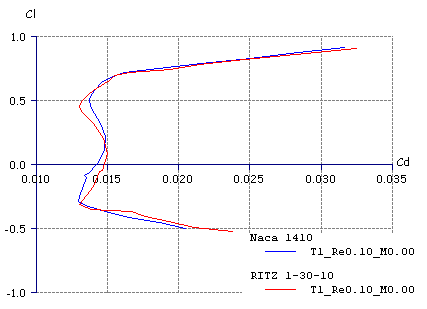
\includegraphics[width=0.8\linewidth]{img-02}
  \caption{Polaires de profil de Type 1}
  \label{img:polaire_type_1}
\end{figure}

\subsubsection{Objet point de fonctionnement (\texttt{OpPoint})}

Un point de fonctionnement d’un profil donné est défini par son angle 
d’attaque et son nombre de Reynolds. Il est toujours associé à un profil
et à un objet Polaire. Le point de fonctionnement comporte les résultats
visqueux et non visqueux de l’analyse.

Un nombre quelconque d’OpPoints peut être enregistré dans la base de 
données créée au moment de l’exécution, la seule limitation étant la
capacité mémoire de l’ordinateur. Les OpPoints peuvent utiliser des
ressources de mémoire importantes. 

Afin d’assurer la cohérence, toute modification du profil ou de la polaire 
entraîne la suppression du point de fonctionnement de la base de données.
\clearpage
\subsubsection{Analyse XFoil}

\begin{figure}[H]
  \centering
  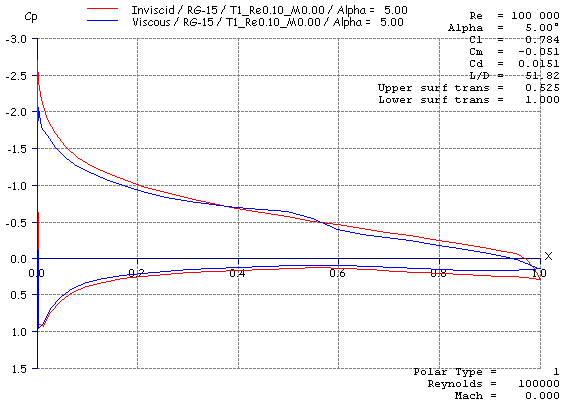
\includegraphics[width=0.8\linewidth]{img-03}
  \caption{Calcul de $Cp$}
  \label{img:calcul_Cp}
\end{figure}

% le §3.2.5}

Chaque fois qu’une analyse XFoil directe est effectuée et que l’on obtient 
une convergence, un OpPoint est généré et les valeurs qui nous intéressent
sont enregistrées dans l’objet polaire actuellement sélectionné. Les données 
sont ajoutées à la polaire, que l’option d’enregistrer les OpPoints ait été 
activée ou pas. 

Un calcul XFoil effectué avec le même d’angle d’attaque et le même Re qu’un 
point de fonctionnement existant le remplacera et les données de la polaire 
seront mises à jour. 

La case à cocher \texttt{Init couche limite} est l’équivalent de \texttt{Init} 
du menu commande de XFoil, c’est-à-dire qu’elle réinitialise la couche limite à
des valeurs standard avant d’effectuer l’analyse. Il est recommandé de cocher cette case lors du premier calcul et lorsque l’analyse d’un OpPoint n’a pas convergé ou est très différente de la précédente.

Dans le cas d’une analyse séquentielle, \texttt{Init couche limite} est automatiquement désactivée après qu’un premier point de convergence a été atteint, et elle est réinitialisée après des calculs n’ayant pas convergé.

\subsubsection{Erreurs de XFoil}

Étant donné la complexité et de la difficulté d’une analyse visqueuse, 
XFoil est remarquablement robuste et cohérent. Il peut cependant arriver que le 
message d’erreur suivant soit généré lors d’une analyse.

Ce message d’erreur est habituellement provoqué par maillage du profil trop grossier, ou un bord d’attaque trop aigu. Il est possible que, dans un tel cas, XFoil soit bloqué et échoue dans toutes ses tentatives pour effectuer une nouvelle analyse. La commande de menu \texttt{Point de fonctionnement/Réinitialiser XFoil} peut être utilisée pour réinitialiser toutes les variables et réinitialiser les profils et les polaires actuellement sélectionnés. 

\begin{figure}[htbp]
\centering
  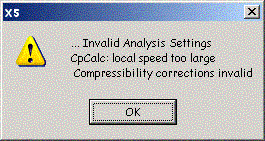
\includegraphics[width=0.4\linewidth]{img-04}
  \caption{Message d’erreur de XFoil}
  \label{img:message_erreur_XFoil}
\end{figure}

\subsubsection{Exemple de session d’analyse directe}

\begin{enumerate}
	\item Lancer l’application \texttt{Analyse directe XFoil} depuis le menu
	\texttt{Fichier}~;
	\item Charger un profil depuis un fichier~;
	\item (Optionnel) Utiliser les commandes \texttt{Annuler la rotation du
	profil} et \texttt{Normaliser le profil} depuis le menu \texttt{Conception}
	pour respectivement aligner la corde moyenne avec l’axe-x et pour définir sa
	longueur à 1~;
	\item (Optionnel) Utiliser les commandes \texttt{Refaire localement le
	maillage} ou \texttt{Refaire globalement le maillage} pour optimiser les
	panneaux du profil~;
	\item Utiliser la commande \texttt{Définir une analyse} depuis le menu 
	\texttt{Analyse}, ou \touche{F6}, afin de  définir une analyse – par
	exemple une analyse de Type 1 à $Re \approx 100~000$ et $Mach = 0.0$~;
	\item Définir un angle d’attaque ou un coefficient de portance à analyser
	– par exemple $ \alpha = 0\degree $~; 
	\item Cliquer le bouton \bouton{Analyser} sur la barre d’outils de droite 
	pour lancer une analyse~;
	\item Si l’analyse XFoil a convergé, la distribution $Cp$ sera
	automatiquement affichée~;
	\item Cocher \texttt{Afficher la couche limite} ou \texttt{Afficher la
	pression} pour visualiser l’une ou l’autre des distributions~;
	\item Cocher la case \texttt{Séquence} sur la barre d’outils de droite~;
	\item Définir les angles min et max de l’analyse – par exemple de 
	$ \alpha = ‑6\degree $ à $ \alpha = 10\degree $~;
	\item Comme la nouvelle valeur de départ est différente de manière
	significative de celle des derniers calculs (par exemple 
	$ \alpha = 0\degree $), cocher \texttt{Init couche limite}~;
	\item Cliquer le bouton \bouton{Analyser}~;
	\item Cliquer le bouton \bouton{Animer} pour visualiser les modifications de
	couche limite ou des distributions de pression en fonction des variations
	de l’angle d’attaque~;
	\item Cliquer la commande \texttt{Polaires} du menu \texttt{Afficher} ou 
	presser \touche{F8}~;
	\item Utiliser le bouton de la souris et la molette pour glisser et zoomer
	les diagrammes.
\end{enumerate}

\subsection{Conception inverse complète [\texttt{MDES}] et Conception inverse mixte [\texttt{QDES}]}

\subsubsection{Généralités}

Les deux modes de conception ne sont pas modifiés par rapport à l’original. 

Les profils créés avec la méthode inverse complète sont définis par 255 points de coordonnées, ce qui est excessif pour les analyses directes qui suivent. Un remaillage du profil est fortement recommandé.

Bien que les profils créés par la méthode inverse mixte aient le même nombre de panneaux que le profil d’origine, un remaillage est quand même conseillé. 

\subsubsection{Exemple de session – Conception inverse complète}
\begin{enumerate}
	\item Aller à l’application \texttt{Inverse complète} (commande de menu ou
	\touche{Ctrl}+\touche{3})~;
	\item Sélectionner un profil depuis la base de données chargée, ou charger
	un profil depuis un fichier~;
	\item Cliquer le bouton \bouton{Nouvelle spline} sur la barre d’outils de
	droite~;
	\item Sélectionner deux points soit sur l’extrados, soit sur l’intrados, 
	mais pas un sur chacune des surfaces~;
	\item Glisser les points de contrôle de la spline pour définir une nouvelle
	distribution de vitesses~;
	\item Cliquer le bouton \bouton{Appliquer la spline} pour enregistrer les 
	modifications~;
	\newcounter{enumTemp}
    \setcounter{enumTemp}{\theenumi}
	\item Cliquer le bouton \bouton{Exécuter} pour lancer le calcul de la 
	géométrie du nouveau profil~;
	\item Utiliser les boutons de la souris et la molette pour glisser et
	zoomer le diagramme et le profil~;
	\item Répéter le processus jusqu’à obtenir la géométrie désirée~;
	\item Pour enregistrer le profil modifié, cliquer la flèche de la barre
	de menu supérieure ou sélectionner \texttt{Enregistrer le profil dans la
	base de données} depuis le menu \texttt{Profil}~;
	\item Passer à l’application \texttt{Analyse Directe} (menu ou \touche{Ctrl}
	+\touche{5})~;
	\item Utiliser \texttt{Refaire globalement le maillage} dans le menu
	 \texttt{Conception} afin de générer un maillage plus grossier\footnote{En 
	 conception inverse, le maillage obtenu comprend 255 points. Il faut donc le
	 dégrader quelque peu sinon xfoil prend trop de temps.}~;
	\item Poursuivre avec l’analyse directe.
\end{enumerate}

\subsubsection{Exemple de session – Conception Inverse Mixte}

Les étapes 1 à \theenumTemp~sont identiques à celles de la méthode de conception \texttt{Inverse complète}.

\begin{enumerate}
	\setcounter{enumi}{\theenumTemp}
	\item Cliquer le bouton \bouton{Marquer pour modification} et définissez 
	quelle partie du profil doit être modifiée~;
	\item Cliquez le bouton \bouton{Exécuter} pour calculer la nouvelle 
	géométrie du profil~;
	\item Vérifier la convergence dans la fenêtre textuelle.\\
	En cas de non convergence, il est possible soit de reprendre les itérations
	en cliquant de nouveau le bouton \bouton{Exécuter}, soit d’exporter la 
	géométrie modifiée telle qu’elle est.
\end{enumerate}

Terminer comme avec la méthode de conception Inverse complète.

\subsection{Conception directe de profil}

\subsubsection{Généralités}

Un module de conception brute a été inclus dans XFLR5, il permet la
conception de profils soit à partir de B-splines, soit sous
forme de points reliés par des splines. Le premier donne des surfaces
plus lisses et le dernier autorise un meilleur contrôle de la géométrie.

Ce mode de conception n’est cependant pas la meilleure manière de concevoir
des profils et les autres possibilités dérivées de XFoil sont bien mieux
adaptées et recommandées, par exemple~:

\begin{itemize}
	\item Modifier l’épaisseur et la cambrure d’un profil~;
	\item Interpoler des profils~;
	\item Méthodes inverses.
\end{itemize}

Ce mode de conception de profil peut cependant être utilisé pour superposer
différents profils afin de comparer leur géométrie.

Une option a été ajoutée à la version v6 qui permet de charger une image
d’arrière-plan, avec l’idée de numériser des profils existants.

\subsubsection{Fonctionnalités principales des B-splines}

L’extrados et l’intrados sont chacun déterminé par une B-spline séparée. 
Le degré de la Spline peut être défini entre 2 et 5.

\subsubsection{Fonctionnalités principales des splines reliant des points}

L’extrados et l’intrados sont chacun déterminé par un jeu de points de 
contrôle.

Les points de contrôle sont reliés par des B-splines du 3e degré.

Deux points de contrôle intermédiaires sont ajoutés à la jonction des deux
splines, respectivement à 1/3 et 2/3 de l’écart entre les deux points de
contrôle. Ces deux points sont automatiquement ajoutés et ne sont pas
visibles. Ils ne peuvent pas non plus être modifiés.

La pente en chaque point de contrôle visible est déterminée par la ligne qui passe par le points de contrôle qui le suit immédiatement et celui qui le précède immédiatement.

\subsubsection{Bord d’attaque et bord de fuite}

Pour chacune des deux méthodes, la pente au bord d’attaque est verticale et ne peut être modifiée. Dans le cas d’une conception à partir de B-splines, ceci est fait en forçant le second point de contrôle à rester sur l’axe vertical.

Dans le cas de \texttt{Points reliés par des splines}, la pente au bord de fuite
est déterminée par la position de deux points supplémentaires situés à l’arrière, un pour chacune des surfaces. 

\subsubsection{Précision en sortie}

Le nombre maximum de points en sortie sur chacune des surfaces est de 150.
Ceci est cohérent avec le dimensionnement des tableaux de XFoil et avec la
précision requise pour l’application, bien que l’augmentation de la puissance
de calcul et de la capacité mémoire des ordinateurs modernes puisse
permettre davantage de points. Typiquement, XFoil exige au moins 50 points
sur chaque face afin d’effectuer une analyse adéquate.

Dans les deux cas, il est prudent de refaire le maillage du profil depuis le menu principal afin d’améliorer la convergence de l’analyse de XFoil et sa précision. Ceci peut être effectué avec l’équivalent des commandes \texttt{PANE} et \texttt{CADD} de XFoil.

À la sortie du module de conception, il sera demandé à l’utilisateur s’il
veut exporter ou pas le profil vers le module d’analyse. 

\subsubsection{Numérisation}
Une option a été ajoutée avec la version v6.02 permettant de charger une
image d’arrière-plan. Le but est de permettre la numérisation d’un profil
existant en utilisant des splines.

Après numérisation, les splines pourront être enregistrées sous forme de
profil dans la base de données, et le profil devra être normalisé, avoir
sa rotation supprimée et être remaillé.

\section{Analyse 3D}

\label{section : analyse 3D}

\subsection{Repères du fuselage et aérodynamique, conventions de signes}

\begin{figure}[htbp]
	\centering
	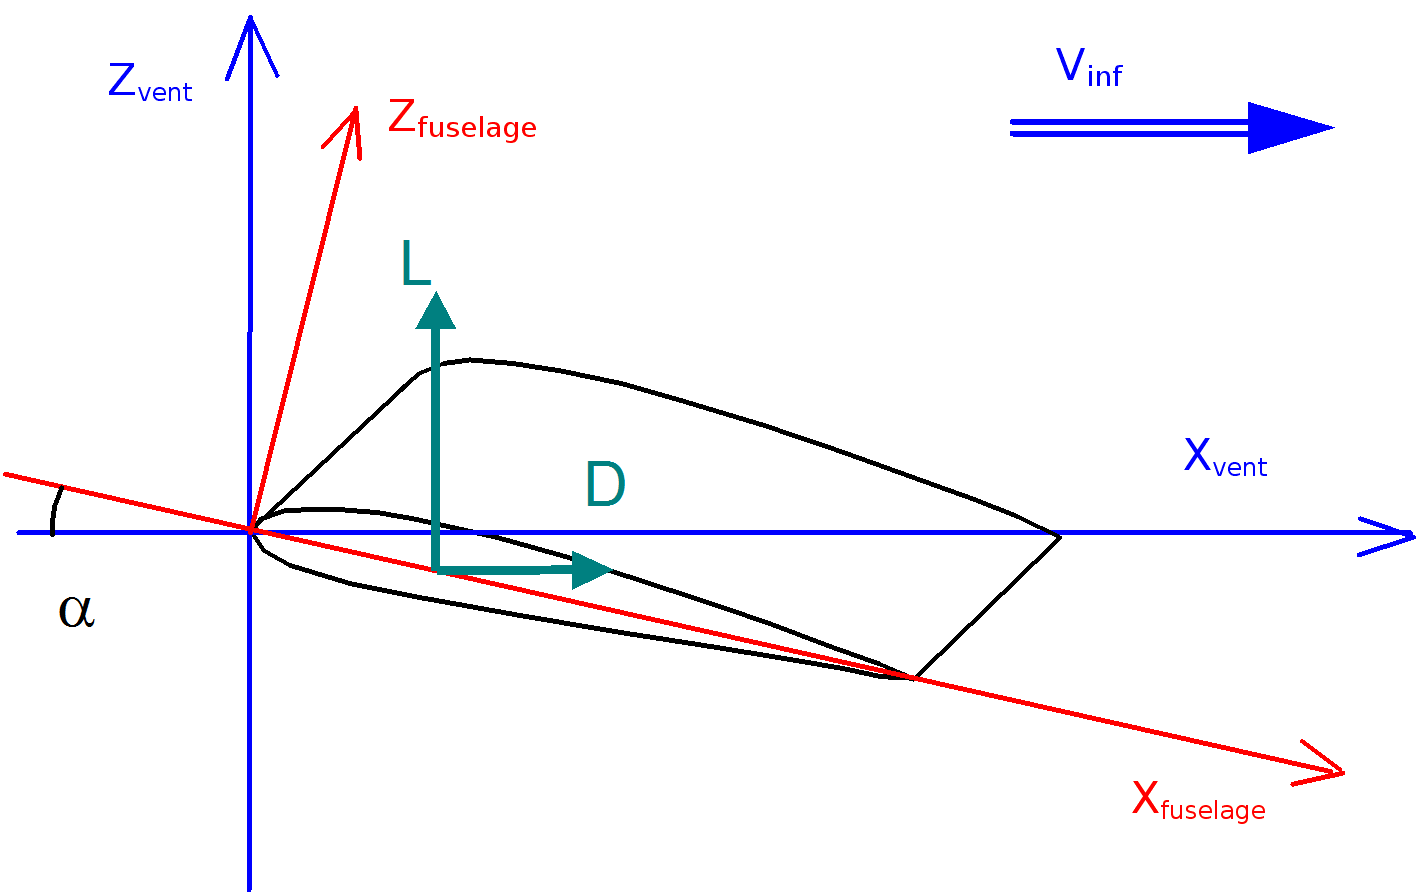
\includegraphics[width=0.8\linewidth]{img-05-fr}
	\caption{Repère aérodynamique et du fuselage}
	\label{img:repères_aérodynamique_fuselage}
\end{figure}

Les coefficient de portance et de traînée sont donnés dans l’axe du vent.
Notes~:
\begin{itemize}
	\item Jusqu’à la v3.21, les calculs étaient faits en utilisant 
	l’approximation des petits angles, ce qui signifie que les repères
	aérodynamique et du fuselage étaient les mêmes~;
	\item Conventions de signe pour les moments – d’après Wikipédia, Flight
	Dynamics\footnote{Ceci est une «~pseudo-citation~», en effet, il n’existe 
	pas de page en français sur Wikipédia correspondant exactement à ce sujet.
	L’article sur la \href{https://fr.wikipedia.org/wiki/Mécanique_du_vol}
	{Mécanique du vol} est à l’état d’ébauche. J’ai donc traduit la partie qui
	nous intéresse [ndt]}~:
	\begin{quotation}
		La convention aéronautique la plus courante définit le roulis comme 
		s’appliquant sur l’axe longitudinal, il est positif lorsque l’aile de
		droite descend. Le lacet est appliqué selon l’axe vertical du fuselage,
		il est positif lorsque le nez est orienté à droite. Le tangage est 
		appliqué  selon un axe perpendiculaire au plan de symétrie longitudinal
		de l’avion, il est positif avec le nez haut.
	\end{quotation}
\end{itemize}

Ceci est illustré par la Figure~\ref{img:conventions_signe_moments}

\begin{figure}[htbp]
	\centering
	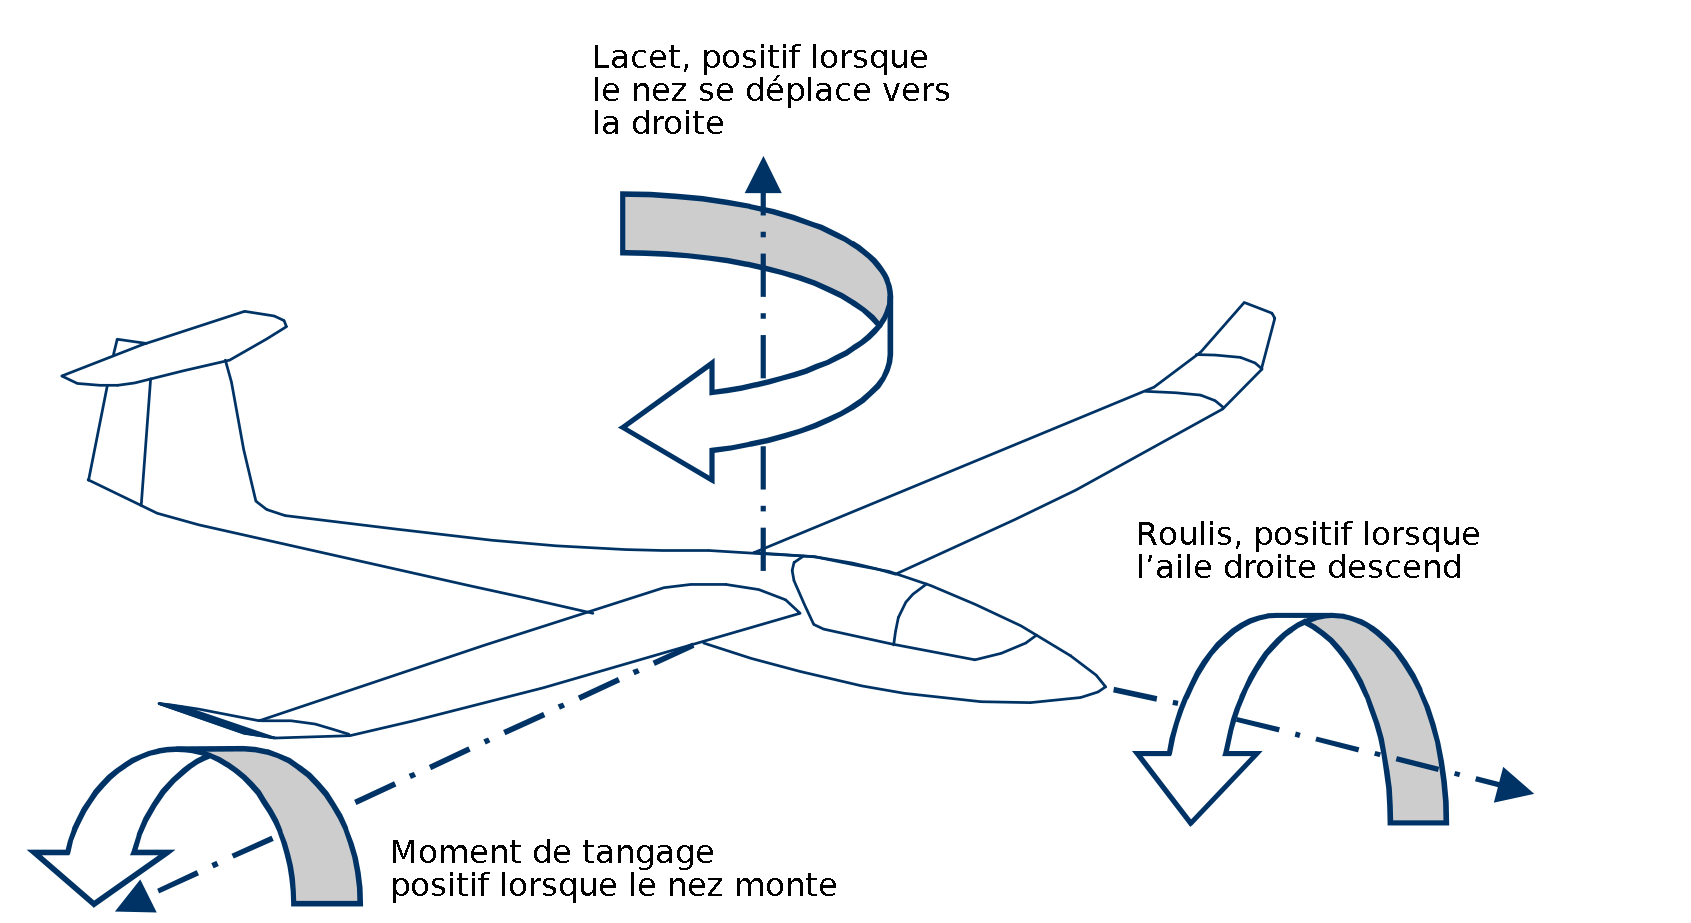
\includegraphics[width=0.8\linewidth]{img-06-fr}
	\caption{Conventions de signe des moments}
	\label{img:conventions_signe_moments}
\end{figure}

\clearpage
\subsection{Définition d’objet}

\subsubsection{Définition de l’aile}

\begin{figure}[!ht] % htbp
	\centering
	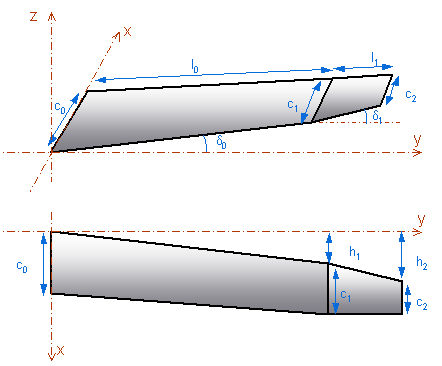
\includegraphics[width=0.8\linewidth]{img-07}
	\caption{Définition de l’aile}
	\label{img:définition_aile}
\end{figure}

L’aile est définie comme un ensemble de panneaux. Chaque panneau est défini
par~:
\begin{itemize}
	\item sa longueur $l_i$~;
	\item les cordes d’emplanture et d’extrémité $c_i$ et $c_{i+1}$~;
	\item le décalage du bord d’attaque aux cordes d’emplanture et d’extrémité
	$h_i$ et $h_{i+1}$~;
	\item l’angle de dièdre $ \delta_\iota$~;
	\item le maillage pour l’analyse VLM.
\end{itemize}

La longueur d’un panneau, le long de l’envergure devrait au moins être égale à la longueur minimum des éléments VLM des autres panneaux. Des divisions par zéro et des résultats non physiques peuvent résulter d’une longueur de panneau
insuffisante. 

Le vrillage\footnote{«~washout~»} est pris en compte par la  LLT comme une modification de l'angle d’attaque. 

En VLM, le vrillage est traité comme une modification de l’aile, le centre de
rotation étant placé au quart de la corde. 

Jusqu’à la version v3.04, le vrillage a été appliqué comme une rotation des 
sections par rapport à l’axe y absolu. Depuis la version v 3.05, les sections 
sont pivotées par rapport au quart de la corde du panneau, c’est-à-dire
après que le panneau a été pivoté de l’angle de dièdre. Les résultats
sont impactés pour les ailes ayant des panneaux bien en dehors du plan x-y.

L’«~envergure~» de l’aile est définie par $$L=2 \times \sum l_i$$

Pour faciliter l’interprétation, l’aile est affichée développée selon un 
plan horizontal, à la fois dans la fenêtre de conception de l’aile et dans
la vue 2D. Seule la vue 3D donne une représentation réaliste de la géométrie. 

Une aile peut être asymétrique si les profils sont différents de chaque côté.
Cette option est destinée à fournir une certaine possibilité d’évaluer l’influence de volets, mais elle doit être utilisée avec précautions. Elle n’a
été testée ni expérimentalement, ni en fonction de résultats théoriques.

\subsubsection{Surface de référence pour les coefficients aérodynamiques}

La surface de référence pour tous les coefficients aérodynamiques de l’aile
et de l’avion est la surface de l’aile principale.

Dans le cas d’un biplan, la surface de référence est aussi la surface de
l’aile principale.

Les longueurs de référence pour les coefficients de moment sont définies au 
\S\ref{section : moments}

\underline{Note~: }
\begin{itemize}
	\item Jusqu’à la version v.4.15, la surface de référence et l’envergure de 
	référence ont été définies comme la surface et l’envergure développées. Avec 
	cette convention, la contribution de winglets est comptée dans la surface et
	dans l’envergure. Ce n’est pas nécessairement le meilleur choix, car il est 
	habituellement pratique de comparer les coefficients de performance d’une 
	aile avec et sans les winglets, mais avec une surface de référence 
	identique~; 
	\item À partir de la version v4.16, l’option par défaut est d’utiliser la 
	surface développée et l’envergure projetées sur le plan xy. Avec cette 
	définition, la contribution de winglets à l’envergure et à la surface est
	nulle. Par commodité, il est encore possible de choisir l’une ou l’autre 
	des surfaces de référence~; l’option peut être définie dans la boîte de 
	dialogue de la définition de l’analyse.
\end{itemize}

\subsubsection{Volets}

Depuis la version v3.16, les méthodes de maillage automatique prennent en 
compte les ruptures au niveau de la position des volets, si les profils
aux deux extrémités du panneau d’aile sont définis avec un volet. 

La manière recommandée pour créer un volet est de définir deux profils 
situés à la même position sur l’envergure, le premier avec une rupture de
volet, l’autre sans. Le code ignorera les panneaux de longueur nulle. 

\begin{figure}[htbp]
	\centering
	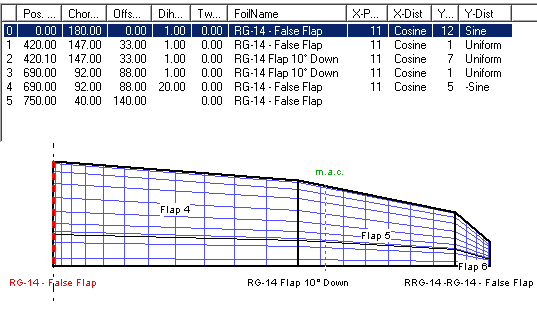
\includegraphics[width=0.8\linewidth]{img-08}
	\caption{Définition des volets}
	\label{img:définition_volets}
\end{figure}

Les volets triangulaires, définis par un profil complet à une extrémité du panneau et par une rupture de volet de l’autre côté, ne sont pas reconnus.

Les volets sont comptés avec un pour chaque aile. Par exemple les ailerons sont comptés comme deux volets. Ceci est nécessaire pour calculer séparément les moments d’articulation pour les ailes asymétriques.

\subsubsection{Conception du fuselage}

La modélisation du fuselage est naturelle avec une méthode de panneaux 3D, mais elle ne se fait jamais sans difficulté.

\paragraph{Options de modélisation}

Deux options sont disponibles, avec deux buts différents~:

\begin{enumerate}
  \item Représentation par panneaux plats~: ceci est le but 
  d’\texttt{Analyse}.\\
  Étant donné un fuselage existant, l’idée est de numériser sa géométrie et de
  l’entrer dans XFLR5. La géométrie résultante ne sera pas lisse mais ceci est
  habituellement suffisant dans un but de prédiction. 
  \item Représentation par B-splines~: ceci est le but de \texttt{Conception}.\\
  L’idée est de définir et d’optimiser la géométrie d’un fuselage pour
  obtenir certaines performances aérodynamiques (ou esthétiques) prévues. Les 
  points du fuselage peuvent ensuite être exportés sous forme d’un fichier texte
  pour une utilisation ultérieure.
\end{enumerate}

\paragraph{Importer et exporter des données de fuselage} 
Pour faciliter le processus de modification, les points de contrôle peuvent être 
édités dans un fichier texte et importés dans XFLR5 plutôt que définis directement dans XFLR5. 

Un exemple de format d’entrée peut être obtenu en exportant une définition 
de fuselage existante.

Un format typique est~: 

\begin{verbatim}
Nom_fuselage
...
FRAME
x_1 y_2 z_1
...
x_n y_n z_n

OFFSET
X_o Y_o Z_o

BODYTYPE
1 or 2
\end{verbatim}

Notes~:
\begin{itemize}
	\item Les mots-clés doivent être précédés du caractère \texttt{\#}
	\footnote{Je ne trouve pas ce caractère dans l’exemple précédent.}~;
	\item \texttt{n} est le nombre de points latéraux définissant un couple de
	fuselage. Ce nombre doit être le même pour tous les couples. Si des couples
	sont définis avec un nombre de points différent, le couple défini en dernier
	définira le nombre de points~;
	\item Les couples sont triés selon les positions en x~;
	\item Les points du couple devraient être définis dans le sens horaire, sur 
	la face gauche du fuselage, lorsqu’on regarde le fuselage de l’avant~; c’est 
	la vue qui est affichée sur le panneau de droite du module de conception du 
	fuselage~;
	\item Tous les points d’un couple devront avoir la même position axiale~;
	\item La position en x d’un couple est définie par le premier point.
\end{itemize}

\subsubsection{Définition d’un avion}

Un avion est constitué d’une aile principale, et de manière optionnelle, d’une
seconde aile, d’un stabilisateur horizontal, de une ou deux dérives et d’un fuselage. Le fuselage peut être décrit soit par des coupes situées à différentes positions dans le sens du flux ou par des surfaces NURBS\footnote{Voir \href{https://fr.wikipedia.org/wiki/NURBS}{cet article sur les NURBS} sur Wikipédia.}.

\paragraph{Assemblage des surfaces}

La difficulté principale lors de la construction d’un modèle d’avion en 3D est de connecter ensemble l’aile, le stabilisateur, la dérive et le fuselage. Sans l’aide d’un système de CAO, il a été difficile d’implémenter un algorithme souple et robuste, principalement en raison du grand nombre de configurations à prendre en compte. Par exemple, le stabilisateur peut avoir ou pas une intersection avec le fuselage, il peut ou pas avoir une intersection avec la dérive et peut n’avoir d’intersection avec le fuselage qu’à son extrados ou son intrados, etc.

La seule vérification de surface implémentée avec la version V4.00 est un ajustement des ailes, du stabilisateur et de la dérive à la surface du fuselage. Même alors, l’algorithme peut ne pas être assez robuste pour toutes les configurations.

De plus, même si les ailes, le stabilisateur et la dérive sont ajustés à la surface du fuselage, les panneaux de fuselage ne sont pas ajustés pour suivre leur contour. Ceci entraîne que certains panneaux du fuselage se trouveront à l’intérieur du volume, ce qui n’est pas cohérent avec la théorie des panneaux.

\paragraph{Éléments d’extrémité d’ailes}

La théorie des panneaux exige que le volume sur lequel sera effectuée l’analyse soit entièrement clos par les surfaces qui supportent les panneaux. En d’autres termes, un fuselage ou une aile ne peut pas avoir d’extrémité ouverte, auquel cas on obtient une erreur de calcul.

Afin d’essayer de clore les volumes, le code créera automatiquement des éléments d’extrémité dans les cas suivants~:

\begin{itemize}
	\item Extrémité gauche de l’aile gauche et extrémité droite de l’aile 
	droite~;
	\item Extrémités haute et basse des dérives.
\end{itemize}

Il ne créera pas d’élément dans les cas suivants~:

\begin{itemize}
	\item Espace au centre de l’aile, c’est-à-dire lorsque la première corde est 
	située à une position positive sur l’envergure~;
	\item Jonction entre l’aile et le fuselage.
\end{itemize}

\underline{Note~:} l’influence de ces erreurs de modélisation sur les résultats est inconnue.

\subsubsection{Estimations de l’inertie}

Un formulaire  de calcul est fourni afin de donner une valeur approximative de la position du CG\footnote{Dans la suite de ce document \textbf{CG} représentera le centre de gravité} et du tenseur d’inertie associé à la géométrie. L’évaluation ne doit pas être comprise comme quelque chose d’autre qu’un ordre de grandeur grossier.

L’inertie est évaluée dans le système de coordonnées par défaut, c’est-à-dire par rapport au CG. Le tenseur dans d’autres repères pourra être calculé en effectuant les transformations appropriées du tenseur.

L’évaluation est basée sur les hypothèses suivantes~:

\begin{itemize}
	\item Pour le fuselage, la masse est répartie uniformément sur la surface  
	extérieure, et cette surface est supposée avoir une épaisseur uniforme. Le 
	fuselage est divisé en $N_b$ sections élémentaires le long de l’axe x. Le 
	poids est concentré au centre de la coupe. Ceci est illustré 
	Figure~\ref{img:masse_fuselage}.
	\item Pour les ailes, la masse est supposée être distribuée de manière 
	uniforme dans le volume de l’aile le long de l’envergure.\\
	Dans XFLR5 v5, ceci a été modélisé sous forme de masses ponctuelles situés 
	au quart de la corde des sections réparties le long de l’envergure.\\
	Dans XFLR5 v6, ceci est modélisé sous forme de masses ponctuelles 
	distribuées à la fois dans la direction de l’envergure et de la corde, comme 
	illustré Figure~\ref{img:masse_aile}.
	\item La répartition de la masse est indépendante du maillage de l’aile 
	utilisé pour les calculs aérodynamiques~;
	\item Des éléments tels que les servos, la batterie, le plomb, ou le 
	récepteur doivent être modélisés séparément comme des masses ponctuelles.
\end{itemize}

\underline{Notes}~:
  \begin{itemize}
	\item À ce stade du développement du code, les résultats ne sont utilisés 
	nulle part dans les calculs de performances. Les évaluations de l’inertie 
	sont fournies comme une commodité pour une analyse externe de la stabilité à 
	effectuer avec des codes tels qu’AVL~;
	\item La masse définie pour les ailes et les fuselages n’est pas celle 
	utilisée pour les calculs de Type 2. La masse pour le Type 2 est définie par 
	l’Analyse/Polaire.
  \end{itemize}

\begin{figure}[htbp]
	\centering
	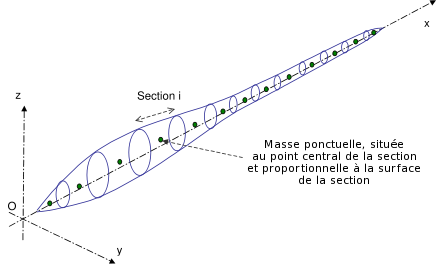
\includegraphics[width=0.8\linewidth]{img-09-fr}
	\caption{Représentation de la masse du fuselage}
	\label{img:masse_fuselage}
\end{figure}

\begin{figure}[htbp]
	\centering
	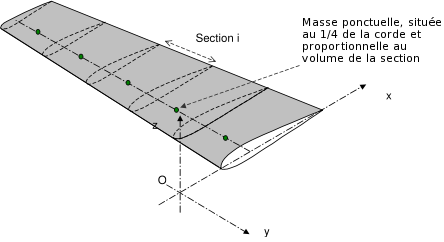
\includegraphics[width=0.8\linewidth]{img-10-fr}
	\caption{Représentation de la masse de l’aile}
	\label{img:masse_aile}
\end{figure}

\subsubsection{Maillage}

L’aile est «~maillée~» en un certain nombre de panneaux répartis le long de l’envergure et de la corde de l’aile développée. Un tourbillon ou un dipôle et une source sont associés à chacun des panneaux.

\begin{itemize}
	\item L’analyse peut être du type VLM, elle est réalisée sur la ligne de 	
	cambrure moyenne.
	\item L’analyse peut être du type panneaux 3D dans laquelle l’aile est 
	modélisés comme une surface épaisse.
\end{itemize}

Il est recommandé de choisir une distribution de panneaux cohérente avec la géométrie de l’aile, c’est-à-dire que la densité du maillage doit être augmentée aux points des ruptures géométriques, ainsi qu’à l’emplanture et à l’extrémité de l’aile. Une distribution de type cosinus est recommandée dans la direction de
la corde afin d’avoir une densité supérieure aux bords d’attaque et de fuite.

Il y a une limite inférieure à la taille des panneaux en dessous de laquelle les calculs deviennent instables, ou conduisent à des résultats n’ayant pas de réalité physique. Ceci se produit typiquement avec les distributions des panneaux de type «~sinus~» le long de l’envergure. Idéalement, la précision des calculs augmente avec la finesse du maillage, mais les temps de calcul augmentent en conséquence. Il est assez simple de faire des essais pour déterminer quel est le meilleur compromis pour un objectif de conception donné.

Une instabilité numérique peut aussi se produire dans l’analyse des panneaux 3D si la longueur des panneaux dans le sens de l’envergure et le long de la corde sont trop différents. Le rapport d’aspect des panneaux doit être maintenu faible.

Il est possible d’exclure des calculs les panneaux d’aile ayant une longueur dans le sens de l’envergure inférieure à une valeur minimum. Ceci peut être défini dans la boîte de dialogue des paramètres avancés. Si la longueur minimum est définie à zéro, alors tous les panneaux d’aile ayant une longueur inférieure à 1/1000 de l’envergure seront exclus. Ceci est destiné à éviter des erreurs de calculs liées à des éléments de maillage de trop petites dimensions.

Méthode des panneaux~:
\begin{enumerate}
	\item L’implémentation actuelle utilise des panneaux plats du 1er ordre.\\
	Idéalement, ce type de panneau doit avoir ses quatre coins dans le même 
	plan, ce qui n’est pas possible pour les géométries vrillées. Cependant, il
	ne semble pas que ce soit un problème majeur pour les faibles vrillages 
	utilisés avec les ailes de modèles réduits de planeurs~;
	\item La vitesse en surface est le gradient d’intensité du dipôle entre des
	panneaux adjacents comme décrit dans la réf \cite{Maskew}. Il est donc 
	recommandé d’avoir le même nombre de panneaux le long de la corde pour toute
	l’envergure, et le même type de distribution, soit uniforme, soit 
	sinusoïdale.\\
	Idéalement, les panneaux devraient partager les mêmes nœuds d’arêtes et de 
	coins. Dans le cas d’un volet, l’astuce pour connecter correctement les 
	panneaux est de définir un profil avec un faux volet positionné à un angle 
	de volet de $0\degree$ comme illustré sur la 
	Figure~\ref{img:maillage_volet}.
\end{enumerate}

\clearpage

\paragraph{Disposition des panneaux - Analyse VLM}

Une attention particulière doit être prise dans la disposition des panneaux VLM afin d’éviter d’avoir un point de contrôle de la surface d’empennage trop proche de la branche arrière d’un tourbillon en fer à cheval de l’aile. Ceci donnerait une division par zéro et des résultats incohérents. 

Une méthode pour éviter ce problème est d’avoir les panneaux d’aile alignés  avec ceux du stabilisateur.

Pour la même raison, c’est une bonne idée, bien que ce ne soit pas obligatoire, de placer les dérives dans les plans de jonction des panneaux d’ailes. 

\begin{figure}[!ht]
	\centering
	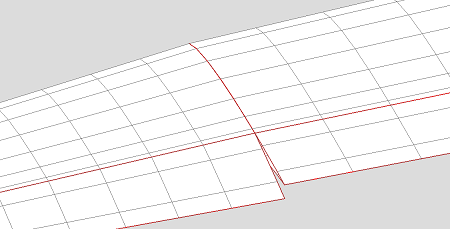
\includegraphics[width=0.7\linewidth]{img-11}
	\caption{Disposition du maillage pour un volet}
	\label{img:maillage_volet}
\end{figure}

\begin{figure}[!ht]
	\centering
	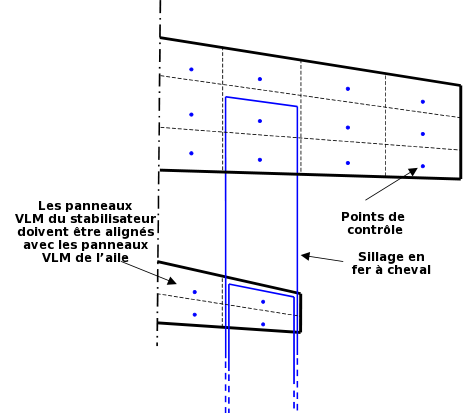
\includegraphics[width=0.7\linewidth]{img-12-fr}
	\caption{Disposition des panneaux VLM pour un avion}
	\label{img:panneaux_VLM_avion}
\end{figure}

\clearpage

\paragraph{Disposition des panneaux – Analyse par panneaux 3D}

\subparagraph{Panneaux le long de la corde}

La distribution $Cp$ est calculée comme la dérivée de l’intensité du dipôle le long de bandes de panneaux dans les directions de la corde et de l’envergure. Pour obtenir ceci, il faut que chaque aile ait un nombre de panneaux de maillage le long de la corde uniforme le long de l’envergure. Il est aussi recommandé que la distribution des panneaux le long de la corde soit la même d’un panneau d’aile à l’autre, c’est-à-dire une distribution cosinusoïdale  pour chaque panneau d’aile. Ceci est nécessaire pour connecter de manière adéquate les panneaux de maillage à la jonction entre les panneaux d’aile.

Les panneaux de maillage placés sur les volets ne sont pas connectés aux panneaux d’aile adjacents. Les connexions restantes à la jonction sont  effectuées selon la méthode décrite dans réf. \cite{Maskew}. 

\subparagraph{Panneaux de sillage}

Dans la méthode VLM, le sillage est représenté par les queues des tourbillons en
fer à cheval. 

Dans la méthode des panneaux 3D, le sillage est modélisé en tant que série de panneaux plats qui s’étendent «~loin derrière~» l’aile. 

L’idée est que, de chaque bande le long de la corde de l’aile, découle une colonne de panneaux de sillage. L’intensité du dipôle de chaque panneau dans cette bande de sillage est la différence entre l’intensité du dipôle des panneaux d’extrados et d’intrados de la bande de l’aile. Ceci est une conséquence du fait que le sillage ne peut pas conserver de charge. De plus, comme il s’agit d’une surface mince, les panneaux de sillage ont une source d’intensité nulle.

Les bandes de sillages sont modélisées sous forme d’une colonne de panneaux  minces. Dans leur forme la plus simple, ces panneaux de sillage sont alignés  directement derrière les panneaux d’aile comme illustré sur la
Figure~\ref{img:sillage_droit}.

\begin{figure}[htbp]
	\centering
	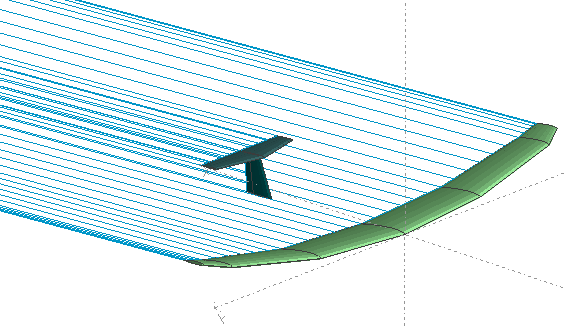
\includegraphics[width=0.8\linewidth]{img-13}
	\caption{Sillage droit}
	\label{img:sillage_droit}
\end{figure}

Dans une implémentation plus fine et plus réaliste, le sillage serait aligné avec les lignes de flux qui se trouvent entraînées derrière l’aile. Comme la distribution des dipôles sur l’aile et les lignes de flux dépendent à leur tour de la forme du sillage, un processus itératif est nécessaire pour atteindre un état de convergence. En général, on appelle ceci «~le processus de relaxation du sillage~».

La relaxation du sillage est un processus difficile qui peut facilement diverger. Des expériences numériques avec XFLR5 ont montré que les panneaux de sillage sont très déformés à l’extrémité des ailes lorsque le sillage s’enroule fortement sur lui-même. La convergence exige un contrôle précis par l’utilisateur de paramètres-clés, comme le nombre de panneaux de sillage, la longueur des panneaux de sillage ou l’intervalle de temps. Pour ces raisons, le processus d’enroulement du sillage a été désactivé.

Les panneaux de sillage sont donc définis comme des panneaux plats qui s’étendent derrière les bords de fuite des ailes. Leur longueur est de 100 x CAM\footnote{CAM = Corde Aérodynamique Moyenne.}. À cette distance, l’influence des panneaux de l’avion est négligeable.

Une difficulté intervient lorsque l’un des panneaux plats de sillage engendré par une surface telle que l’aile rencontre une autre surface comme le stabilisateur, ce qui est illustré Figure~\ref{img:interférences_sillage}a. Ceci va conduire à des résultats irréalistes, non physiques. 

Dans ces conditions, il est nécessaire de modifier légèrement la géométrie pour éviter les interférences Figure~\ref{img:interférences_sillage}b.

\begin{figure}[htbp]
	\centering
	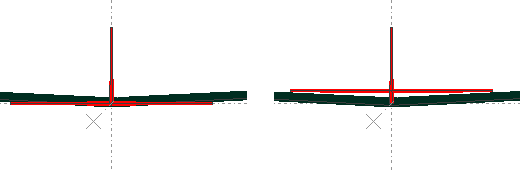
\includegraphics[width=0.8\linewidth]{img-14}
	\caption{a et b~: Interférences du sillage entre l’aile et le stabilisateur}
	\label{img:interférences_sillage}
\end{figure}

\subsubsection{Symétrie}
\label{symétrie}
Un calcul symétrique réduit la taille de la matrice de moitié environ (à 
l’exception de la dérive), et réduit les opérations d’inversion de matrice
par un facteur 4. Le code détecte automatiquement si le problème est
symétrique ou pas. Il est considéré comme étant symétrique dans les cas
suivants~:

\begin{itemize}
	\item l’aile est symétrique lors des calculs d’aile seule~;
	\item l’avion est symétrique sans la dérive ou avec une double dérive.
\end{itemize}

Sinon, le problème est asymétrique~:
\begin{itemize}
	\item si l’aile, la profondeur ou la dérive est asymétrique~;
	\item si l’avion possède une dérive.
\end{itemize}

\subsection{Analyse des performances}

\subsubsection{Théorie – Généralités}

XFoil permet d’avoir une idée unique du comportement des profils, mais c’est 
une analyse 2D, donc le résultat est celui d’une aile d’allongement infini 
et définie avec un seul profil. L’influence que l’allongement seul peut avoir 
sur les polaires de l’aile, indépendamment de la flèche ou du dièdre, justifie 
une analyse plus évoluée de l’aile 

\begin{figure}[htbp]
  \centering
  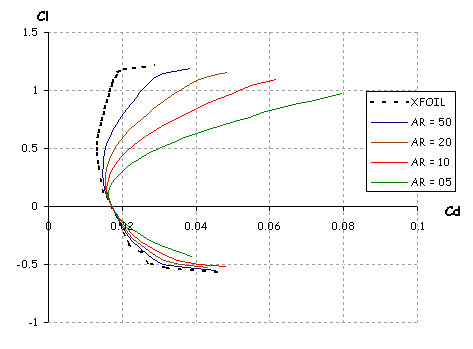
\includegraphics[width=0.8\linewidth]{img-15}
  \caption{Influence de l’allongement - Calculs LLT profil NACA 3412 –
  Effilement = 1 – Flèche = 0$\degree$}
  \label{img:influence_allongement}
\end{figure}

L’aile peut être calculée par l’une quelconque des trois méthodes, chacune 
ayant ses propres avantages et toutes ayant certaines limites d’utilisation.

La première est la méthode de la ligne portante, dérivée de la théorie de 
l’aile de Prandtl. La seconde est la méthode Vortex Lattice. La troisième est 
une méthode de panneaux 3D.

L’originalité des implémentations est leur couplage avec les résultats des 
calculs de XFoil pour estimer la traînée visqueuse associée à l’aile, bien 
que cela soit fait de différentes manières selon la méthode. 

\subsubsection{Calculs visqueux et non visqueux}

Dans les méthodes VLM et de panneaux, une analyse/polaire non visqueuse peut 
être définie, dans ce cas, il n’est pas nécessaire de définir un maillage 
polaire pour les profils. Les caractéristiques visqueuses seront définies à 
zéro.

La LLT est obligatoirement visqueuse. 

\subsubsection{Théorie de la ligne portante (LTT\protect\footnote{LLT~: Lifting Line Theory}) – Non linéaire}

\paragraph{Généralités}

Une LLT «~classique~» est linéaire, c’est-à-dire que la relation $ Cz = 
f(\alpha) $ est linéaire et les effets visqueux ne sont pas pris en compte.
Dans l’application présente, une LLT non linéaire a été implémentée. Elle
est basée que la note technique NACA 1269 \cite{Sivells47}.
Citation de la note technique 1269\footnote{Là encore, la citation est ma traduction personnelle avec toute ses imperfections (ndt)}~:

\begin{quotation}
	L’hypothèse sur laquelle est basée la théorie est qu’une aile portante peut
	être remplacée par un ligne portante et que les tourbillons incrémentaux
	engendrés le long de l’envergure traînent derrière l’aile sous forme de 
	lignes droites dans la direction du vecteur-vitesse du flux en espace libre.
	L’intensité de ces tourbillons de traînée est proportionnelle au taux de 
	changement de la portance le long de l’envergure. Les tourbillons de traînée 
	induisent une vitesse normale à la direction de la vitesse en espace libre.
	L’angle d’attaque effectif de chaque section de l’aile a donc pour 
	différence par rapport à l’angle d’attaque géométrique la valeur de l’angle
	(appelé angle d’attaque induit) dont la tangente est le rapport entre la
	valeur de la vitesse induite et la valeur de la vitesse en espace libre. 
	L’angle d’attaque effectif est donc lié à la distribution de la portance par 
	l’intermédiaire de l’angle d’attaque induit. De plus, l’angle d’attaque 
	effectif est lié au coefficient de portance du profil selon les données des 
	profils à deux dimensions utilisés pour l’aile. Les deux relations doivent
	être satisfaites simultanément dans le calcul de la distribution de la 
	portance de l’aile.

	Si les courbes de portance des profils sont linéaires, leurs relations 
	peuvent être exprimées par une simple équation qui peut être résolue de 
	manière analytique. En général, cependant, les courbes de portance des 
	profils ne sont pas linéaires, particulièrement aux angles d’attaque élevés,
	et des résolutions analytiques ne sont pas faisables. La méthode de calcul 
	de la distribution de portance le long de l’envergure en utilisant des 
	données de profil d’aile non linéaires demande alors de calculer par 
	approximations successives la distribution de portance jusqu’à ce que l’on
	en trouve une qui satisfasse simultanément les relations mentionnées 
	précédemment.
\end{quotation}

\clearpage

Dans l’implémentation actuelle, le comportement de la portance non linéaire est
interpolé à partir des maillages pré-générés de polaires de Type 1 de XFoil et la non linéarité est résolue par une boucle itérative~:

\begin{center}
\begin{tikzpicture}
	\tikzstyle{debutfin}=[ellipse,draw,text=red]
	\tikzstyle{instruct}=[rectangle,draw=black, fill=yellow!50, text 
	width=6cm,text centered]
	\tikzstyle{test}=[diamond, aspect=2.5,thick, draw=black, 
	fill=yellow!50,text=black, text width=3cm, text centered]
	\tikzstyle{es}=[rectangle,draw,rounded corners=4pt,fill=blue!25]

	\node[instruct] (a1) at (-2,20.25) {Définition de l’aile};
	\node[instruct] (a2) at (-2,19) {Sélection des paramètres $\alpha_i$ 
	$V_\infty$};
	\node[instruct] (a3) at (-2,17.5) {Initialisation de $\alpha_i$ avec la
	solution linéaire de la LLT};
	\node[instruct] (a4) at (-2,15.5) {Interpolation de $Cz$ à partir de
	($\alpha + \alpha_i + vrillage, R_e$) sur le maillage polaire de Type 1};
	\node[instruct] (a5) at (-2,13.25) {Si analyse de Type 2, mise à l’échelle
	de $V_\infty$ afin de créer une portance opposée au poids};
	\node[instruct] (a6) at (-2,11.25) {Calcul de la distribution non linéaire
	de $\alpha_i$};
	\node[instruct] (a7) at (-2,9.25) {Interpolation de $Cz$ à partir de
	($\alpha +\alpha_i + vrillage, R_e$) sur le maillage polaire de Type 1};
	\node[instruct] (a8) at (-2,7) {Si analyse de Type 2, mise à l’échelle
	de $V_\infty$ afin de créer une portance opposée au poids};	
	\node[test] (test) at (-2,4.25) {Boucle jusqu’au critère $|\Delta~\alpha_i|$};
	\node[instruct] (a9) at (-2,1.5) {Depuis $\alpha + \alpha_i + vrillage$,
	interpoler le maillage polaire de Type 1, valeurs de $Cx, Cm, etc.$};

	\tikzstyle{suite}=[->,>=stealth,thick,rounded corners=4pt]	

	\draw[suite] (a1) -- (a2);
	\draw[suite] (a2) -- (a3);
	\draw[suite] (a3) -- (a4);
	\draw[suite] (a4) -- (a5);
	\draw[suite] (a5) -- (a6);
	\draw[suite] (a6) -- (a7);
	\draw[suite] (a7) -- (a8);
	\draw[suite] (a8) -- (test);
	\draw[suite] (test) -| (3,4.5) |- (-1.75,12.15) -- (a6);
	\draw[suite] (test) -- (a9);
\end{tikzpicture}
%	\caption{Implémentation de la LLT}
	\label{diagramme : implémentation LLT}
\end{center}

%\begin{figure}[htbp]
%	\centering
%	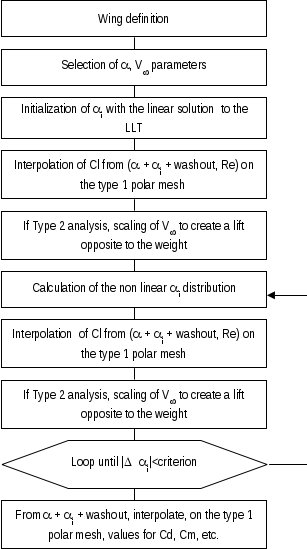
\includegraphics[width=0.5\linewidth]{dia-01}
%	\label{diagramme : implémentation LLT}
%\end{figure}

\clearpage

\begin{figure}[htbp]
	\centering
	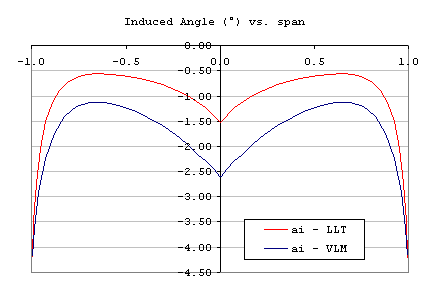
\includegraphics[width=0.8\linewidth]{img-16}
	\caption{Angle induit – Bi-Profil NACA3412-NACA1410 – $AR = 14.8$ – $TR =
	2.0$ – $Alfa = 5\degree$ - $V= 16.7m/s$}
	\label{img:angle_induit}
\end{figure}


\paragraph{Limitations de la LLT}

Il est important de noter que la théorie de la ligne portante possède deux 
limitations importantes. Citation de la note technique 1269\cite{Sivells47}~: 

\begin{quotation}
  Les calculs sont sujets aux limitations de la théorie de la ligne portante
  et il ne faut pas en attendre des résultats précis avec les ailes de
  faible allongement et ayant une flèche importante.
\end{quotation}

De plus, la forme développée de l’aile est supposée reposer essentiellement 
sur le plan X-Y, c’est-à-dire avec un faible dièdre. 

\paragraph{Précautions avec la LLT}

Il s’avère que la convergence de la LLT non linéaire n’est pas un processus 
robuste. Il demande l’utilisation avec précautions d’un facteur de
relaxation. Ce facteur devrait toujours être supérieur à 1. Une valeur de
20 est en général un bon point de départ, et pourra être augmentée au besoin
pour la convergence.

Habituellement, les ailes de faible allongement ont besoin d’une valeur de 
relaxation élevée. 

Le nombre de points d’interpolation le long de l’envergure de l’aile devrait être choisi aux alentours de 20, mais il pourra être augmenté jusqu’à 40. Des nombres plus grands n’améliorent pas la précision de l’analyse mais tendent 
fortement à compromettre la convergence. Le facteur de relaxation devra
être augmenté en fonction du nombre de points d’interpolation le long de l’envergure.

\paragraph{2D par rapport à 3D}

La LLT suppose implicitement que toutes les surfaces se trouvent 
essentiellement sur le plan X-Y. 

Dans cette implémentation de la LLT, la seule utilisation de la flèche et le dièdre se trouve dans le calcul du coefficient de moment de tangage $Cm$. 

La flèche et le dièdre ne sont pas utilisé dans les calculs de la 
distribution de portance. 

\paragraph{Calculs visqueux et non-visqueux}

Il n’y a pas d’option proposée pour effectuer des calculs de LLT non visqueuse. La raison en est que la théorie linéaire requiert qu’un angle de portance nulle soit défini pour chaque profil, et qu’il n’y a aucune manière commode de définir cette valeur de $\alpha_0$ qui dépend du nombre de Reynolds. 
    
\paragraph{Centre de pression de la portance}

Jusqu’à la version v3.11, la position du centre de portance pour chaque
emplacement sur l’envergure était calculée en utilisant l’approximation
usuelle pour les profils minces. C’est-à-dire~:
$$ X_{cp} = 0,25 - \frac{Cm_0} {Cz} $$

Depuis la version v3.12, la position en x du centre de pression de l’aile est calculée par interpolation de la position du centre de pression du maillage de la polaire du profil.

Pour les maillages de polaire de profil générés avant la version v3.05, le 
centre de pression du profil n’était pas enregistré, la formule ci-dessus
étant utilisée pour calculer le centre de pression de l’aile.

\paragraph{Déflexion du flux d’air vers le bas\protect\footnote{«~downwash~» en anglais}}

La déflexion du flux d’air vers le bas est définie à chaque point d’interpolation le long de l’envergure par~:

$$ V_i = V_\infty \cdot \sin \left(\alpha_i \right) $$

Pour des raisons pratiques, il est représenté au bord de fuite de l’aile 
dans les vues 3D. 

\subsubsection{Vortex Lattice Method (VLM) - Linéaire}

\paragraph{Principes généraux de la VLM}
Une méthode VLM a été implémentée en remplacement pour l’analyse des 
géométries d’ailes tombant hors des limitations de la LLT.

Les différences principales avec la LLT sont~:
\begin{itemize}
	\item Les calculs de la distribution de portance, les angles induits et la
	traînée induite sont non-visqueux et linéaires, c’est-à-dire qu’ils sont 
	indépendants de la vitesse de l’aile et des caractéristiques visqueuses de 
	l’air. 
	\item La méthode est applicable à n’importe quelle géométrie d’aile, 
	y-compris celles ayant une flèche, un faible allongement ou un fort dièdre,
	y-compris des winglets. 
\end{itemize}

Le principe de la VLM est de modéliser les perturbations générées par 
l’aile sous la forme d’une somme de tourbillons répartis sur la forme développée de l’aile. L’intensité de chacun des tourbillons est calculée pour se
conformer aux conditions aux limites appropriées\footnote{Conditions aux
limites = Boundary Conditions — \textbf{BC}.}, c’est-à-dire des conditions
de non pénétration de la surface des panneaux. 

Une description complète des principes de l’analyse VLM est largement en
dehors de l’objet de ce document. Seules les fonctionnalités principales
nécessaires à la compréhension du code sont détaillées ci-après. 

La résolution du problème VLM demande l’inversion d’une matrice carrée de 
la taille du nombre de panneaux. Cette inversion est effectuée par une
méthode de pivot partiel de Gauss. La taille du problème peut être réduite
de manière significative par les considérations de symétrie détaillées au
\S\ref{symétrie}.

\begin{figure}[htbp]
	\centering
	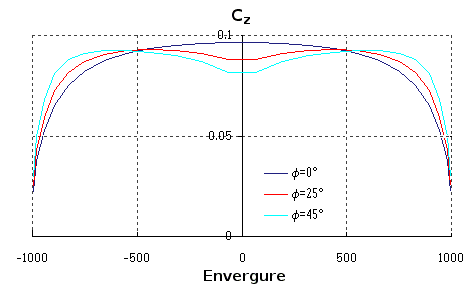
\includegraphics[width=0.8\linewidth]{img-17-fr}\centering 
	\caption{Influence de la flèche pour un $Cz$ donné –  AR=10 – TR=1 –  
	Profil symétrique\protect\footnotemark}
	\label{img:influence_flèche}
\end{figure}

\footnotetext{AR : Aspect Ratio, il s’agit de l’allongement~; TR : Taper Ratio, il s’agit de l’effilement.}

\paragraph{Force de portance et coefficients de portance}
La force agissant sur chacun des panneaux est le produit croisé du vecteur~:
$$ F = \rho V \times \Gamma $$
\begin{itemize}[label=]
	\item $\Gamma$ étant l’intensité du tourbillon $\times$ sa longueur
	\item $\rho$ est la densité du fluide
	\item V est la vitesse en flux libre
\end{itemize}

Ce qui implique que la force est normale à chacun des panneaux.

Le coefficient de portance est défini par~:
$$Cz = \frac {1} {\rho S V^2} \underset{panneaux}\sum F_{wz} $$

\begin{itemize}[label=]
	\item S est la somme des surfaces des panneaux, c’est-à-dire la surface de
	la forme développée
	\item $F_{wz}$ est la projection sur l’axe vertical du repère aérodynamique
\end{itemize}

Cette formule est applicable à la fois à une bande le long de la corde et à 
la surface totale de l’aile.

Les moments de tangage et la position du centre de pression à chaque 
position sur l’envergure sont calculés en faisant la somme de la portance
sur les panneaux.

\paragraph{Limitations de la VLM}

\begin{enumerate}
	\item Les algorithmes de VLM calculent d’abord le coefficient de portance 
	$Cz$ et les autres valeurs qui peuvent être calculées par intégration des 
	forces de surfaces, c’est-à-dire les coefficients de moment et la position
	du centre de pression. Les variables visqueuses ($Cx$ visqueux, t
	transitions, etc.) sont interpolées depuis la valeur de $Cz$ provenant des
	polaires générées précédemment par XFoil.\par
	Ceci soulève un problème de manière évidente pour les valeurs élevées et 
	faibles de $Cz$, lorsque la courbe de la polaire de Type 1 devrait être 
	interpolée soit avant, soit après l’angle de décrochage.\par
	Les résultats de la VLM ne devraient donc pas être pris en compte autour des
	valeurs de l’angle d’attaque proches des angles de décrochage.
	\item Dans sa formulation actuelle, la VLM fait l’hypothèse d’un faible 
	angle d’attaque. Une conséquence majeure est que les tourbillons de traînée 
	ne sont pas alignés avec le vecteur-vitesse en flux libre. Ceci signifie que 
	la matrice d’influence sera indépendante de l’angle d’attaque.\par
	Pour explorer cette limitation, il est possible de tester un calcul de 
	géométrie inclinée, comme c’est expliqué au 
	\S\ref{section : geometrie inclinee}. Les résultats tendent à monter que 
	l’hypothèse des faibles angles d’attaque est acceptable.
\end{enumerate}

\clearpage

\paragraph{Méthode VLM de remplacement}

Dans la méthode VLM «~classique~», un tourbillon en fer à cheval est positionné
au quart de la corde du panneau et la condition de non-pénétration est définie 
au point situé aux trois-quart de la corde. 

\begin{figure}[htbp]
	\centering
	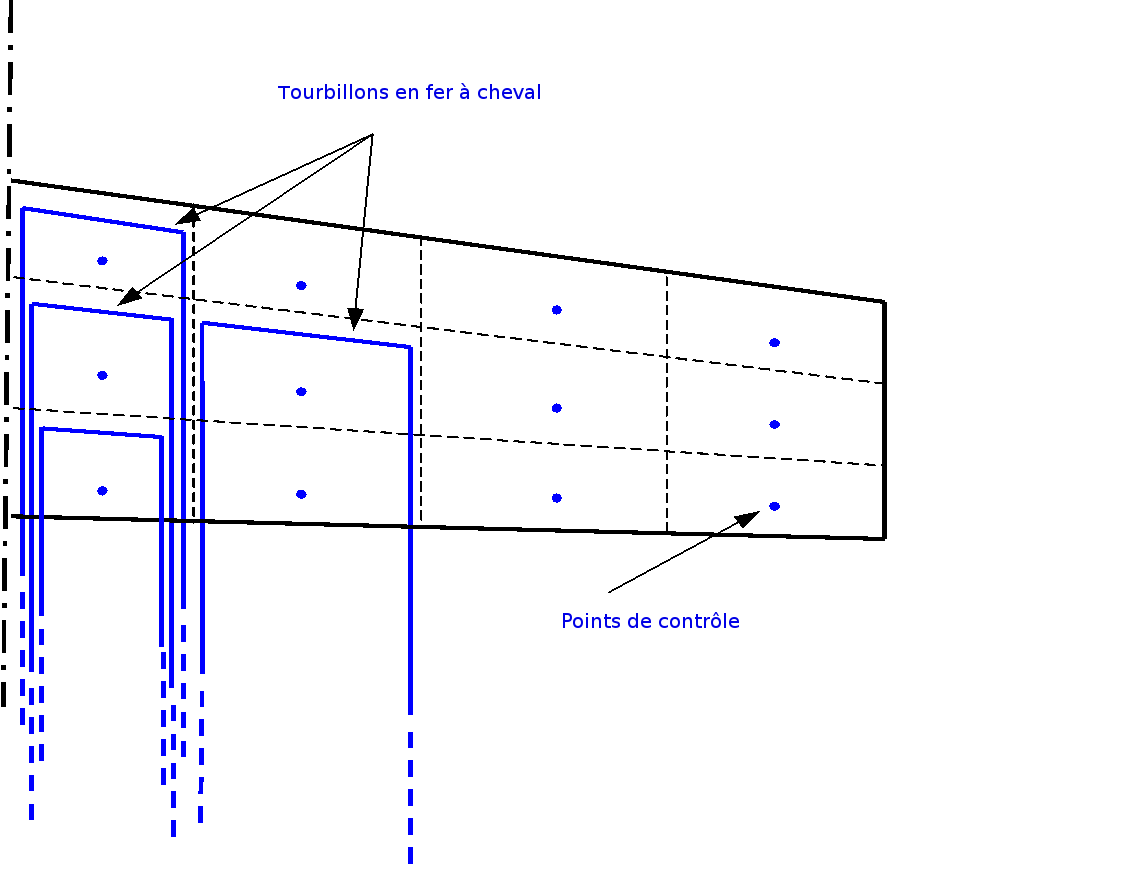
\includegraphics[width=0.7\linewidth]{img-18-fr}
	\caption{Méthode VLM classique}
	\label{img:VLM_classique}
\end{figure}

Dans la méthode recommandée par Katz et Plotkin \cite{Katz}, seuls les tourbillons de traînée s’étendent à l’infini.

Comme le sillage doit être libre de force, l’intensité du tourbillon de traînée est égale à celle du tourbillon quadrangulaire de bord de fuite.

Les deux méthodes sont implémentées dans un but de comparaison mais elles donnent des résultats très proches sinon identiques dans la plupart des cas.

\paragraph{Disposition des panneaux pour la VLM}

La résolution du système et la détermination des intensités des tourbillons demande une inversion de matrice. Dans quelques rares cas, il se trouve que cette matrice est une matrice singulière en raison de la disposition conflictuelle des panneaux et des points de contrôle de la forme développée de l’aile.

Le problème se produit lorsqu’un point de contrôle est situé en ligne avec un tourbillon. Ceci donnera une division par zéro. Dans ces cas, un remaillage manuel des panneaux de l’aile est suffisant pour corriger le problème. Si les problèmes d’inversions persistent malgré le remaillage, il sera nécessaire de vérifier la cohérence des données d’entrée.

\begin{figure}[htbp]
	\centering
	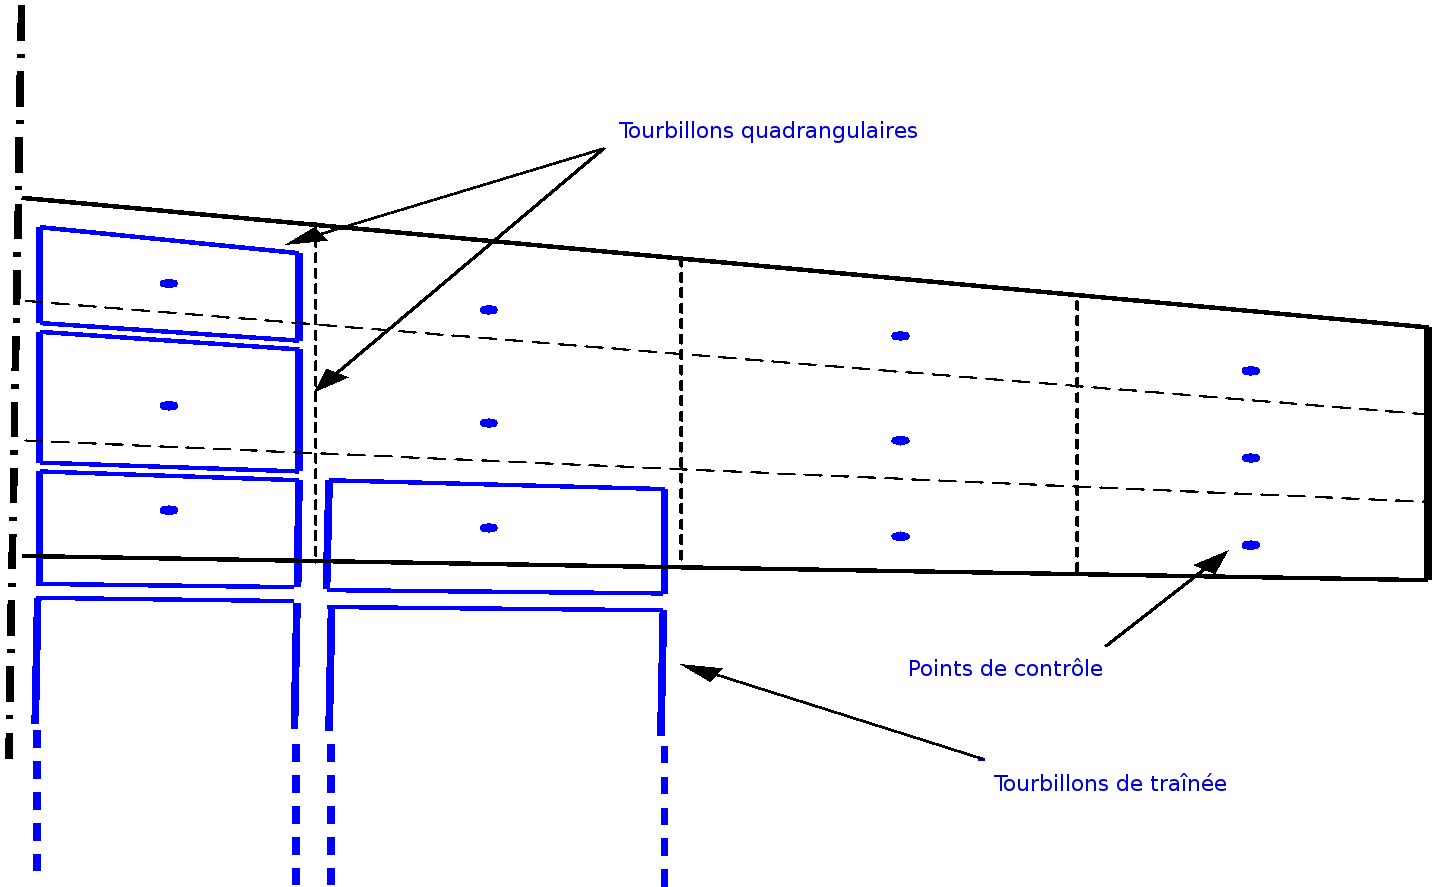
\includegraphics[width=0.7\linewidth]{img-19-fr}
	\caption{Méthode VLM quadrangulaire}
	\label{img:VLM_quad_1}
\end{figure}

\begin{figure}[htbp]
	\centering
	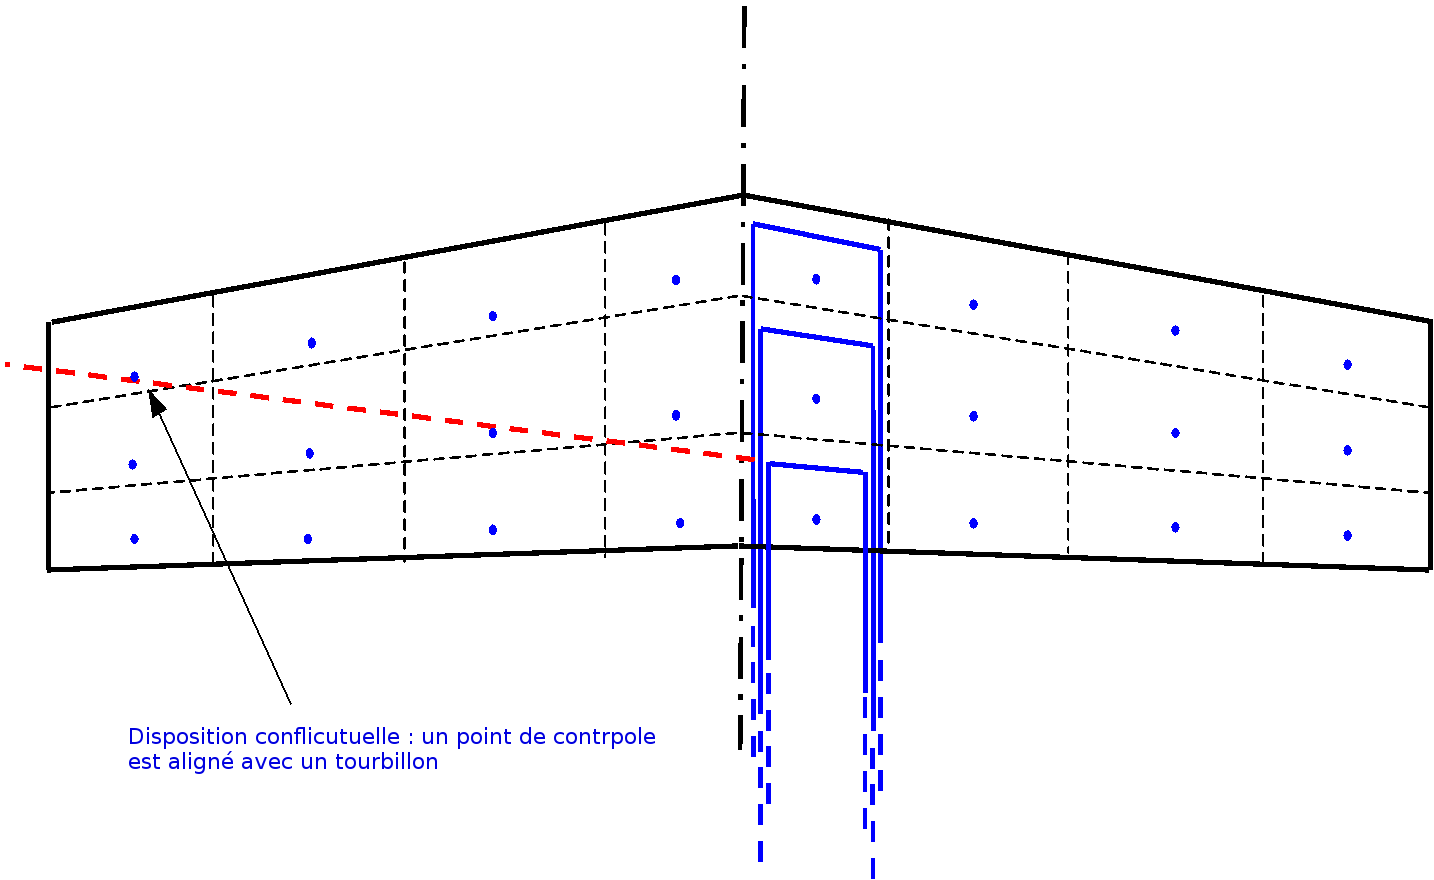
\includegraphics[width=0.7\linewidth]{img-20-fr}
	\caption{Méthode VLM quadrangulaire}
	\label{img:VLM_quad_2}
\end{figure}

\clearpage

\subsubsection{Méthode des panneaux 3D – Linéaire}

\paragraph{Principes généraux}

La méthode des panneaux 3D a été implémentée avec les objectifs suivants~:

\begin{itemize}
	\item affiner les résultats de LLT et de VLM par une méthode plus 
	sophistiquée en 3D complète, prenant en compte l’épaisseur de l’aile, alors 
	que la VLM ne prend en compte que la ligne de cambrure moyenne~;
	\item donner une idée de la répartition de $Cp$ sur l’extrados et 
	l’intrados d’une aile~;
	\item donner une méthode capable de modéliser des fuselages.
\end{itemize}

Le principe de la méthode des panneaux 3D est de modéliser la perturbation engendrée par l’aile par une somme de dipôles et de sources répartis sur l’extrados et l’intrados de l’aile. L’intensité des dipôles et des sources est calculée pour satisfaire aux conditions aux limites appropriées, qui peuvent être du type Dirichlet ou Neumann. 

Une description complète des principes d’une telle méthode va bien au-delà de l’objet de ce document. Seules les fonctionnalités principales nécessaires à une utilisation avisée du code seront détaillées ci-après. La méthode 3D implémentée dans XFLR5 est telle que décrite dans la référence \cite{Maskew}. Pour ceux que cela intéresse, ce document passe en revue l’ensemble des aspects théoriques et numériques de la méthode. 

\paragraph{Méthodes des panneaux 3D dans XFLR5~v6}

Dans XFLR5 v6, pour un panneau de type 3D, les ailes sont modélisées
différemment selon que l’analyse est effectuée pour une aile isolée ou
pour un avion complet~:

\begin{itemize}
	\item pour l’analyse d’une aile isolée, l’aile est modélisée comme une 
	surface épaisse et la méthode 3D complète décrite en \cite{Maskew} est 
	appliqueé~;
	\item pour l’analyse d’un avion, le fuselage/corps est pris en compte, et 
	les ailes sont modélisées comme des surfaces fines~; ceci est une 
	restriction due à l’impossibilité de générer les connexions appropriées 
	entre l’aile et le fuselage sans l’aide d’un programme de CAO 3D.
\end{itemize}

Dans la référence \cite{Maskew}, les auteurs proposent de modéliser la circulation sur les ailes en utilisant des dipôles d’intensité uniforme, et en plaçant la condition aux limites de type Neumann au point de collocation, c’est-à-dire le barycentre ou centre de gravité du panneau. L’alternative est d’utiliser une méthode VLM, et de placer un tourbillon au 1/4 de la corde du panneau, et le point de conditions aux limites aux 3/4 de la corde.

Les deux méthodes ont été testées, et la seconde s’est montrée plus précise et fiable. En conséquence, la méthode de panneaux-3D retenue pour les avions est un modèle mixte de source/dipôle uniforme pour les corps épais, et de tourbillons en fer à cheval pour les surfaces minces.

\paragraph{Résolution du problème}

La résolution du problème des panneaux demande l’inversion d’une matrice carrée dont la taille est le nombre de panneaux. Cette inversion est effectuée par une décomposition LU\footnote{Voir une explication de la 
\href{https://fr.wikipedia.org/wiki/Décomposition_LU}{méthode de décomposition LU} sur Wikipédia.}.

\paragraph{Enroulement du sillage}

Le processus d’enroulement du sillage a été implémenté et testé. Cependant, il n’est pas considéré comme étant suffisamment robuste pour pouvoir être diffusé pour l’instant, et il a été désactivé dans la version v4.00.

\paragraph{Conditions aux limites}

Dans un calcul VLM, les conditions aux limites sont forcément de type Neumann, c’est-à-dire que la composante du vecteur-vitesse normale à la surface doit être nulle. 

Dans un calcul de Panneaux 3D, les conditions aux limites peuvent être soit 
de type Neumann, soit de type Dirichlet. Dans le dernier cas, le potentiel de 
vitesse à la surface interne du panneau est nul, de manière à ce que le potentiel total à l’intérieur du fuselage soit égal au potentiel de vitesse en flux libre.

Après un processus par essais et erreurs, la recommandation est d’utiliser 
la condition aux limites de Dirichlet plutôt que celle de Neumann. Cette 
dernière méthode est plus sensible aux modifications locales de géométrie 
et donne des résultats moins convaincants. C’est aussi le choix implicite
dans la référence \cite{Maskew}.

\paragraph{Validation}

\subparagraph{Analyse d’un cylindre infini et d’une sphère}

Les valeurs théoriques des coefficients $Cp$ pour un corps plongé dans un 
flux uniforme sont~:

\begin{itemize}
	\item pour un cylindre~: $Cp = 1.0$ au bord d’attaque et au bord de fuite 
	et $Cp = -3.0$ au point le plus haut et au point le plus bas~;
	\item Pour une sphère~: $Cp$ = 1.0 au bord d’attaque et au bord de fuite et 
	$Cp = -1.25$ au point le plus haut et au point le plus bas.
\end{itemize}

Ces valeurs sont calculées au \% près par l’analyse de panneaux 3D.


\begin{figure}[H]
	\centering
	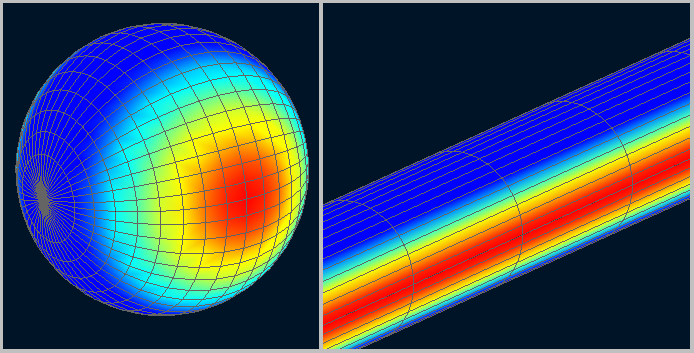
\includegraphics[width=0.7\linewidth]{img-21}
	\caption{Analyse du coefficient de pression — Sphère et cylindre presque
	infini}
	\label{img:analyse_coefficient_pression_1}
\end{figure}

\begin{figure}[H]
	\centering
	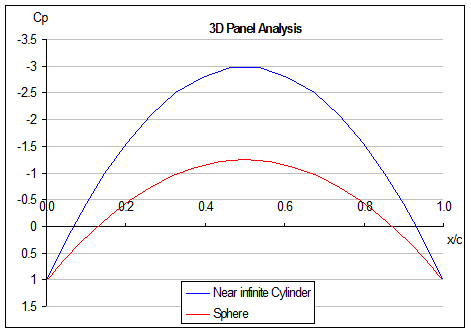
\includegraphics[width=0.7\linewidth]{img-22}
	\caption{Analyse du coefficient de pression — Sphère et cylindre presque
	infini}
	\label{img:analyse_coefficient_pression_2}
\end{figure}

\clearpage

\subparagraph{Analyse d’aile}

La distribution de $Cp$ est calculée par l’analyse des panneaux 3D pour une aile presque infinie, et par l’analyse des panneaux 2D avec XFoil, elles sont tracées dans Figure~\ref{img:analyse_coef_pression_naca2412} et dans 
Figure~\ref{img:analyse_coef_pression_naca64A410}. il y a une concordance générale pour les résultats non visqueux.

\begin{figure}[H]
	\centering
	\begin{subfloat}
		\centering
		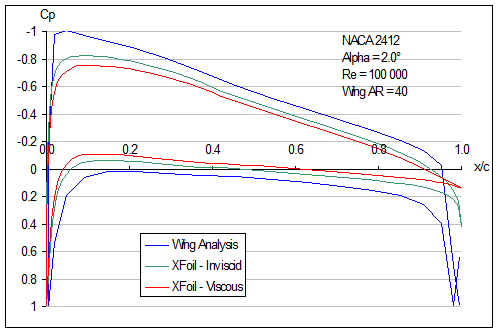
\includegraphics[width=0.7\linewidth]{img-23}
		\caption{Analyse du coefficient de pression – NACA2412}
		\label{img:analyse_coef_pression_naca2412}
	\end{subfloat}

	\begin{subfloat}
		\centering 
		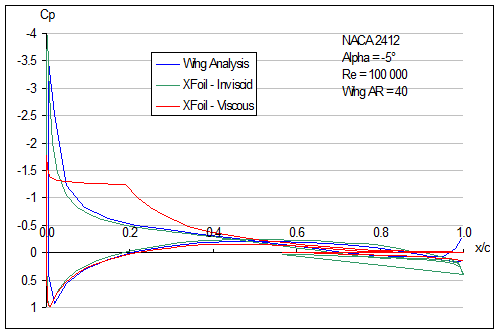
\includegraphics[width=0.7\linewidth]{img-24}
		\caption{Analyse du coefficient de pression – NACA64A410}
		\label{img:analyse_coef_pression_naca64A410}
	\end{subfloat}
\end{figure}

\subsubsection{Considérations d’analyse}

\paragraph{Limitations générales}
En tant que règle générale, la LLT comme la VLM sont adaptées à des
configurations ayant des surfaces portantes minces, travaillant à des angles
d’attaque faibles.

L’hypothèse de l’algorithme de conception de l’aile la plus sujette à caution est probablement l’application des résultats de transition de XFoil aux ailes ayant un allongement fini. La simulation 2D proposée par XFoil correspond à des ailes infinies, où le bulbe laminaire s’étend indéfiniment le long de l’envergure. Certains auteurs suggèrent que sur des ailes à l’allongement limité, de tels bulbes n’apparaissent que sur une partie de la forme développée. Cependant, les théories pour les transitions 3D sont encore au stade du développement et, à la connaissance de l’auteur, ne donnent pas encore totale satisfaction.

La méthode qui consiste à interpoler les résultats générés par XFoil est clairement une approximation et n’a pas de réel fondement théorique ni expérimental, mais elle semble être une approximation raisonnable pour les ailes ayant un allongement modéré à élevé.

Les caractéristiques visqueuses seront de moins en moins représentatives au 
fur et à mesure que  la géométrie de l’aile différera de l’aile idéale 2D infinie de XFoil. En conséquence, ces résultats pour les géométries non planes, les faibles allongements ou les fortes flèches devront être envisagés avec précaution. 

\clearpage 

\paragraph{Sélection d’une méthode d’analyse}

Il faudrait toujours préférer la méthode LLT si la géométrie de l’aile est cohérente avec les limitations de la théorie. LLT donne une meilleure idée de la traînée visqueuse, donne une meilleure estimation du comportement au voisinage des conditions de décrochage aux angles d’attaque élevés, et elle est mieux prise en compte par les travaux théoriques publiés. La méthode des panneaux 3D devrait être sélectionnée si l’on est intéressé par la distribution de $Cp$ sur l’extrados et l’intrados ou si l’influence du fuselage doit être prise en compte.

L’analyse VLM est préférable dans tous les autres cas.

La comparaison de la distribution de $Cp$ à deux positions sur l’envergure 
avec différentes méthodes d’analyse est donnée dans les 
Figure~\ref{img:comparaison_cp_pour_différentes_méthodes_analyse_1} et
Figure~\ref{img:comparaison_cp_pour_différentes_méthodes_analyse_2}.

\begin{figure}[htbp]
	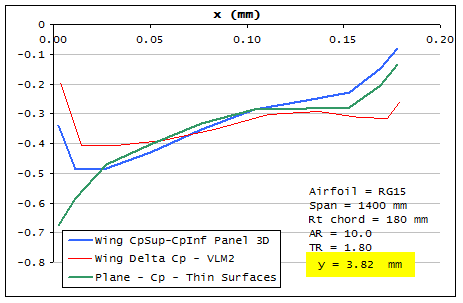
\includegraphics[width=0.7\linewidth]{img-25}\centering 
	\caption{Comparaison de $Cp$ pour différentes méthodes d’analyse}
	\label{img:comparaison_cp_pour_différentes_méthodes_analyse_1}
\end{figure}

\begin{figure}[htbp]
	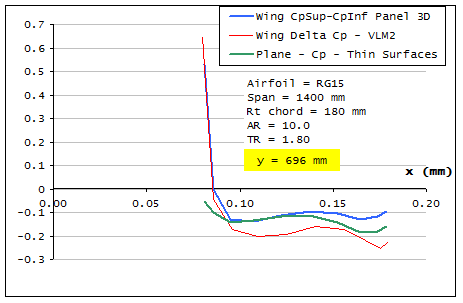
\includegraphics[width=0.7\linewidth]{img-26}\centering 
	\caption{Comparaison de $Cp$ pour différentes méthodes d’analyse}
	\label{img:comparaison_cp_pour_différentes_méthodes_analyse_2}
\end{figure}

\clearpage

\paragraph{Rayon de noyau du tourbillon\protect\footnote{Un tourbillon théorique a une vitesse infinie en son centre. Physiquement, les effets visqueux font que le comportement central n’est pas celui d’un tourbillon pur. Numériquement, on met une approximation linéaire ou constante sur la vitesse.}}

Dans l’analyse VLM, le vecteur-vitesse induit par un tourbillon est singulier sur la ligne de tourbillons.

Dans une méthode de panneaux 3D, le vecteur-vitesse est singulier dans l’alignement des côtés du panneau. Ceci crée des erreurs numériques dans l’analyse et dans les calculs des lignes de courant. Il est donc fortement recommandé de définir un rayon de noyau de tourbillon minimum, qui peut être typiquement de l’ordre de grandeur de $1/1000$ de la taille minimum des panneaux du maillage, par exemple, \emph{rayon de noyau du tourbillon =} $10^{-6}m$. C’est la valeur définie par défaut, elle peut être modifiée dans les paramètres avancés.

La vitesse au point situé sur la ligne de tourbillon, ou dans l’alignement 
d’un côté de panneau, est nulle. 

\paragraph{Dérapage}

La simulation du dérapage a été introduite dans XFLR5 v4.09.

L’ordre dans lequel l’angle d’attaque et le dérapage sont appliqués à son
importance. Dans XFLR5, le dérapage est modélisé en pivotant le modèle autour
de l’axe z, avec un vecteur-vitesse en espace libre demeurant dans le plan x-z. La géométrie résultante est analysée en utilisant les méthodes conventionnelles de VLM et de panneaux. L’avantage de cette méthode est que les tourbillons de traînée sont dans le plan vertical qui contient le vecteur-vitesse, c’est-à-dire qu’ils sont alignés avec l’axe x du repère aérodynamique.

\begin{figure}[htbp]
	\centering
	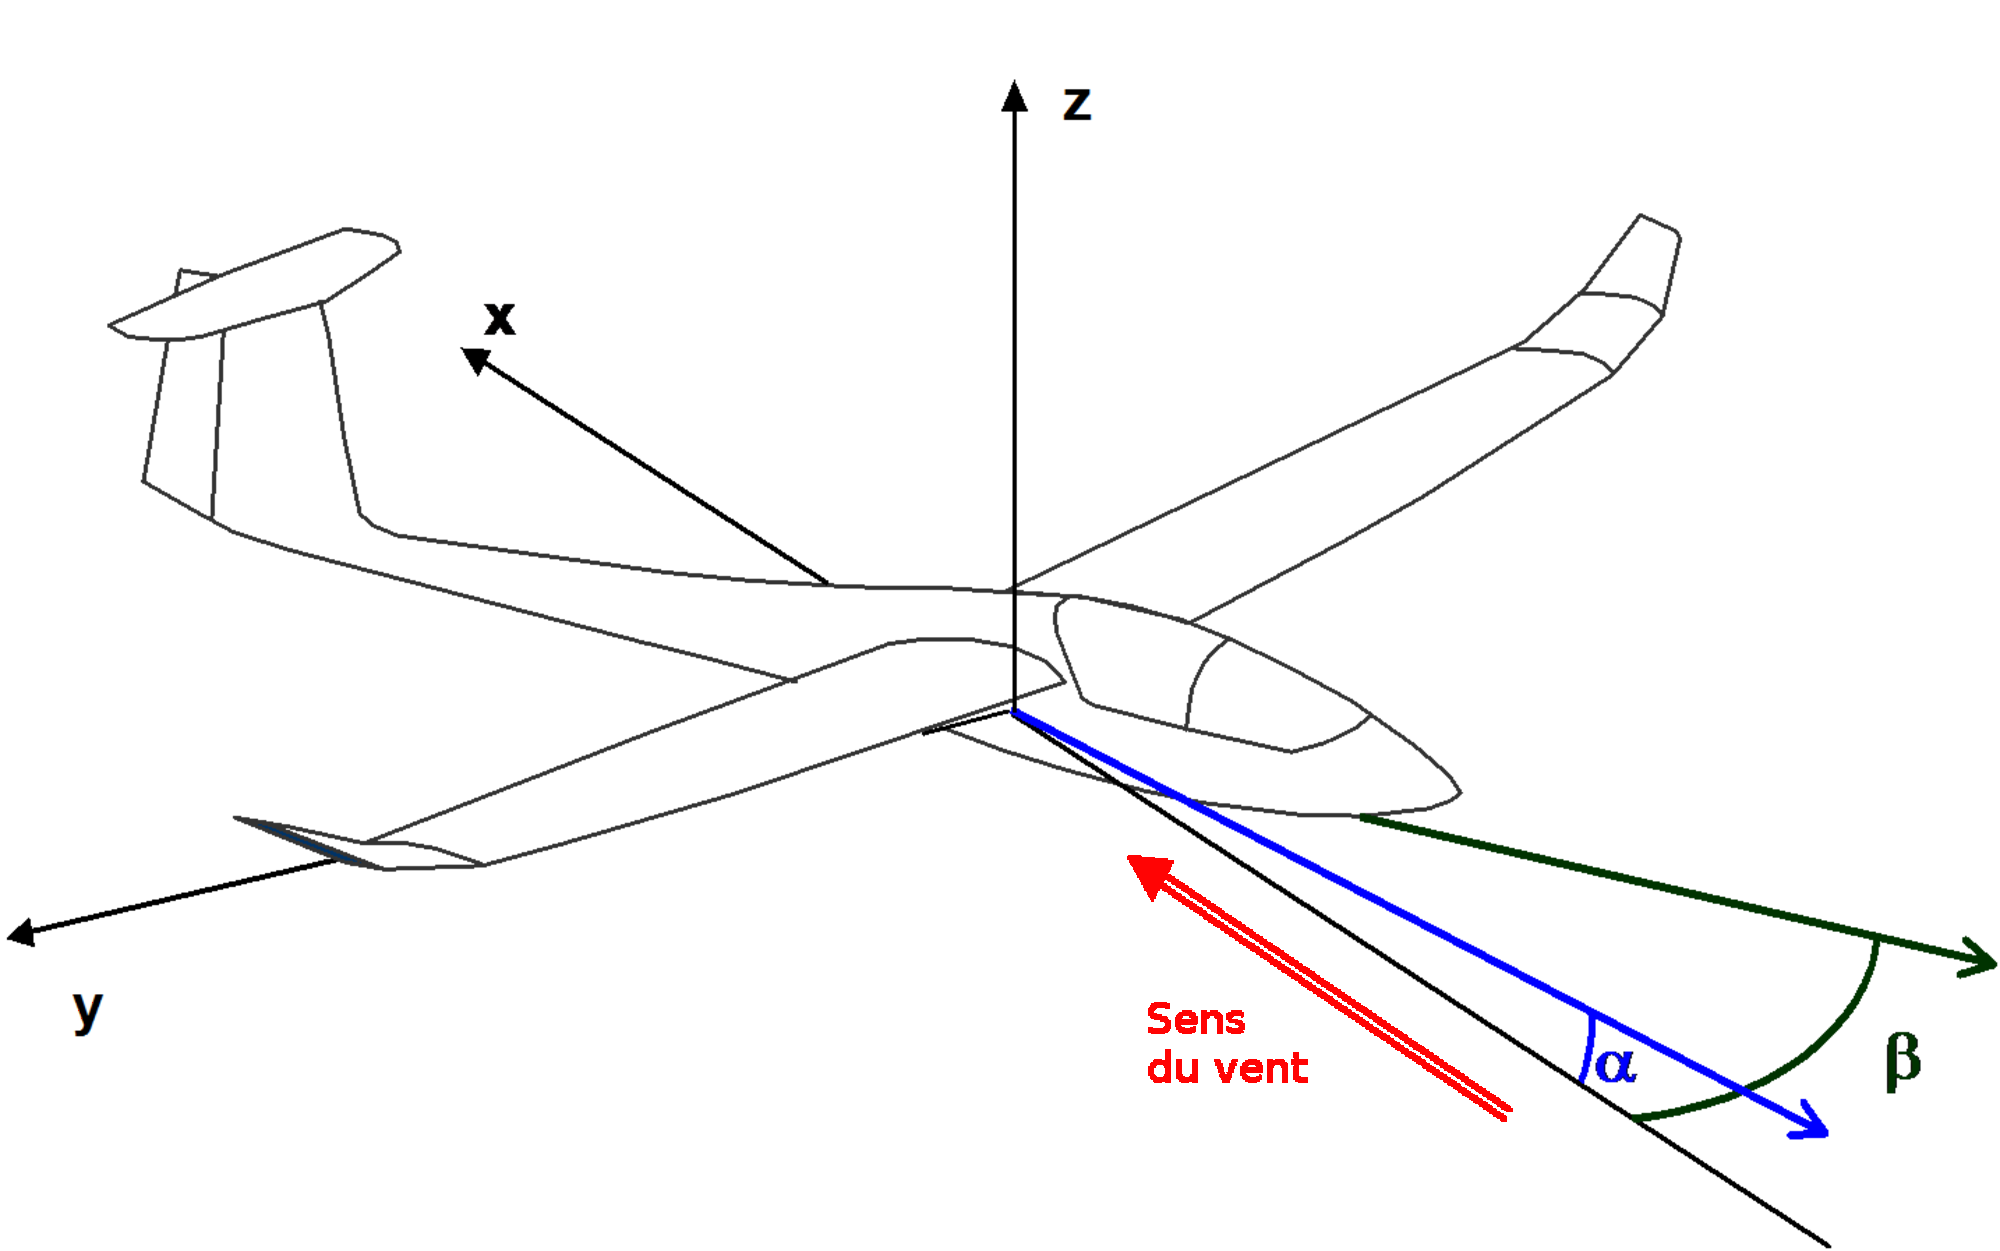
\includegraphics[width=0.8\linewidth]{img-27-fr}
	\caption{Définition du dérapage}
	\label{img:définition_dérapage}
\end{figure}

\paragraph{Plan de Trefftz, analyse en champ lointain et en champ proche} 
La portance et la traînée induite peuvent être calculés par les méthodes du champ proche ou du champ lointain. Les aspects théoriques sont trop vastes pour être détaillés ici, mais en essence, la méthode du champ proche consiste à intégrer les forces de pression sur les panneaux, alors que la méthode du champ lointain est basée sur l’équilibre du moment sur une surface de contrôle située bien en dessous du fuselage, c’est-à-dire le plan de Trefftz.

Il est généralement signalé que les résultats de portance et de traînée de  l’analyse du champ proche sont beaucoup plus élevés et moins représentatifs que ceux résultats des calculs dans le plan de Trefftz. Ce problème n’est pas spécifique à l’implémentation actuelle, il est signalé pour la plupart des codes de VLM ou de panneaux. L’implémentation du code actuel pour les calculs de la portance et de la traînée est donc la méthode du champ lointain.

D’un autre côté, l’analyse du champ lointain ne donne pas d’information sur la distribution de pression sur la bande, et aucune information sur le moment de tangage par rapport au 1/4 de la corde. Tous les moments et la position du centre de pression sont donc calculés en effectuant la somme sur les panneaux. 

Dans l’implémentation actuelle de la méthode des panneaux 3D, on considère que seule l’aile produit un sillage et pas le fuselage. 

\clearpage

\paragraph{Comportement linéaire et non-linéaire}
Les analyses traditionnelles VLM et de panneaux ne prennent pas en compte l’effet visqueux. Pour des modèles réduits fonctionnant à quelques m/s cependant, la traînée visqueuse n’est pas négligeable comparée à la traînée induite et doit donc être estimée avec une autre méthode.

Dans l’application actuelle, la traînée visqueuse est estimée en interpolant les polaires pré-générées de XFoil, par la valeur de $Cz$ résultant de l’analyse linéaire 3D. Ceci suppose implicitement que le comportement du profil d’une aile finie n’est pas très différent d’une «~aile infinie de XFoil~». Il n’y a pas vraiment de support, ni théorique, ni expérimental pour supporter cette approche, elle doit donc être utilisée avec précautions.

Comme c’est généralement le cas en transposant des résultats 2D vers une analyse 3D, l’estimation de la traînée visqueuse est probablement trop faible et peut donner des résultats sans aucun doute optimistes. 

Parce que la VLM est linéaire, elle ne prend pas en compte correctement, entre autre, le décrochage aux grands angles d’attaque, contrairement, potentiellement à la LLT.

\begin{figure}[!ht]
	\centering
	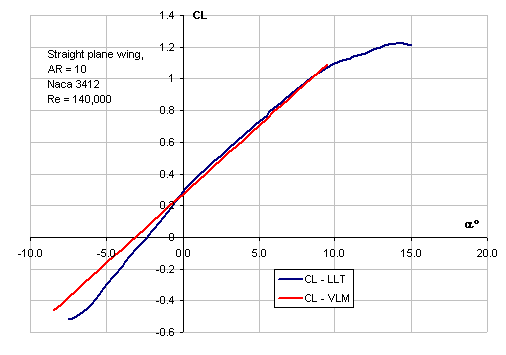
\includegraphics[width=0.8\linewidth]{img-28}
	\caption{Modélisation linéaire et non linéaire}
	\label{img:modélisation_linéaire_non_linéaire}
\end{figure}

\clearpage
\paragraph{Implémentation non linéaire}

%\begin{figure}[h!]
%  \centering
% 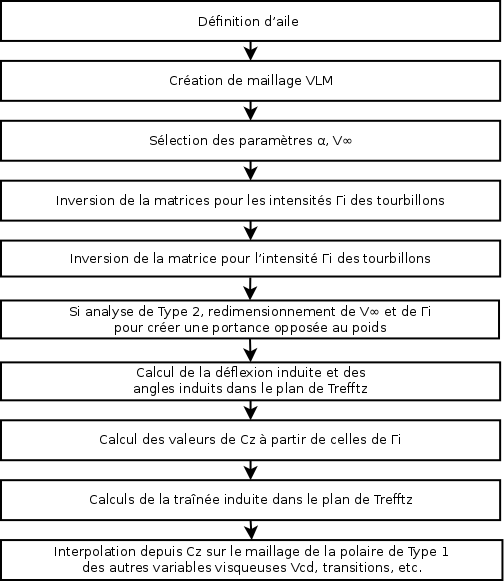
\includegraphics[width=0.7\linewidth]{dia-02-fr}
%  \label{diagramme : tilted geometry}
%\end{figure}

\begin{center}
\begin{tikzpicture}
	\tikzstyle{debutfin}=[ellipse,draw,text=red]
	\tikzstyle{instruct}=[rectangle,draw=black, fill=yellow!50, text 
	width=6cm,text centered]
	\tikzstyle{test}=[diamond, aspect=2.5,thick, draw=black, 
	fill=yellow!50,text=black, text width=3cm, text centered]
	\tikzstyle{es}=[rectangle,draw,rounded corners=4pt,fill=blue!25]

	\node[instruct] (a1) at (-2,20.25) {Définition de l’aile};
	\node[instruct] (a2) at (-2,19) {Création du maillage VLM};
	\node[instruct] (a3) at (-2,17.75) {Sélection des paramètres $\alpha_i$ 
	$V_\infty$};
	\node[instruct] (a4) at (-2,16) {Création de la matrice d’influence du
	tourbillon et des conditions aux limites};
	\node[instruct] (a5) at (-2,14) {Inversion de la matrice pour les
	intensités $\Gamma_i$ des tourbillons};
	\node[instruct] (a6) at (-2,11.5) {Si analyse de Type 2, redimensionnement
	de $V_\infty$ et des $\Lambda_i$ afin de créer une portance opposée au 
	poids};
	\node[instruct] (a7) at (-2,8.75) {Calcul de la déflexion induire de l’air
	vers le bas et des angles induits dans le plan de Trefftz};
	\node[instruct] (a8) at (-2,6.5) {Calcul des valeurs de $Cz$ pour les 
	$\Lambda_i$};	
	\node[instruct] (a9) at (-2,4.5) {Calcul de la traînée induite dans le plan
	de Trefftz};
	\node[instruct] (a10) at (-2,2) {Interpolation depuis $Cz$ sur le 
	maillage de la polaire de Type 1 des autres variables visqueuses $V_cd$, 
	transitions, etc.};

	\tikzstyle{suite}=[->,>=stealth,thick,rounded corners=4pt]	

	\draw[suite] (a1) -- (a2);
	\draw[suite] (a2) -- (a3);
	\draw[suite] (a3) -- (a4);
	\draw[suite] (a4) -- (a5);
	\draw[suite] (a5) -- (a6);
	\draw[suite] (a6) -- (a7);
	\draw[suite] (a7) -- (a8);
	\draw[suite] (a8) -- (a9);
	\draw[suite] (a9) -- (a10);
\end{tikzpicture}
%	\caption{Implémentation de la LLT}
	\label{diagramme : implementation non lineaire}
\end{center}

\paragraph{Géométrie Inclinée – Analyse VLM et panneaux 3D}
\label{section : geometrie inclinee}

La méthode de base VLM utilise l’approximation des petits angles pour la 
définition du sillage. Dans le cadre de cette hypothèse, le sillage est aligné avec l’axe du fuselage~:

\begin{itemize}
	\item pour la VLM, les jambes de traînée des tourbillons en fer à cheval 
	sont parallèles à l’axe x du fuselage~;
	(Figure~\ref{img:configuration_géométrie_normale_inclinée}a)
	\item Pour l’analyse par les panneaux 3D, les panneaux de traînée de sillage 
	sont dans le plan x-y.
\end{itemize}

L’avantage de cette approximation est sa simplicité~: il ne faut qu’une seule
matrice d’influence pour tous les angles d’attaque, et l’inversion de la matrice peut être effectuée simultanément pour tous les alphas.

Le désavantage est que les tourbillons en fer à cheval ou les panneaux de sillage ne sont pas alignés sur le vecteur-vitesse en flux libre.

Une approche plus représentative est d’aligner le sillage avec le repère du vent (Figure~\ref{img:configuration_géométrie_normale_inclinée}b). De manière équivalente, le problème peut être défini dans le repère du vent et la géométrie du fuselage peut être inclinée de l’angle d’attaque 
(Figure~\ref{img:configuration_géométrie_normale_inclinée}c), ce qui est une transposition directe de la physique du problème. Les deux méthodes sont équivalentes, mais la dernière peut être plus facilement implémentée, elle a donc été choisie pour XFLR5. Elle est sélectionnée en cochant «~Incliner la géométrie~» dans la boîte de dialogue d’analyse.

L’inconvénient de cette approche est que cette nouvelle matrice doit être 
définie et inversée pour chacun des angles d’attaque, ce qui conduit à des
temps de calcul plus importants.

Les coefficients $Cz$ et $Cx$ sont sensiblement identiques avec les deux 
méthodes, ce qui signifie que l’approximation des petits angles est valable
du point de vue de l’analyse des performances. Les coefficients de moment
peuvent être légèrement différents.

\begin{figure}[htbp]
	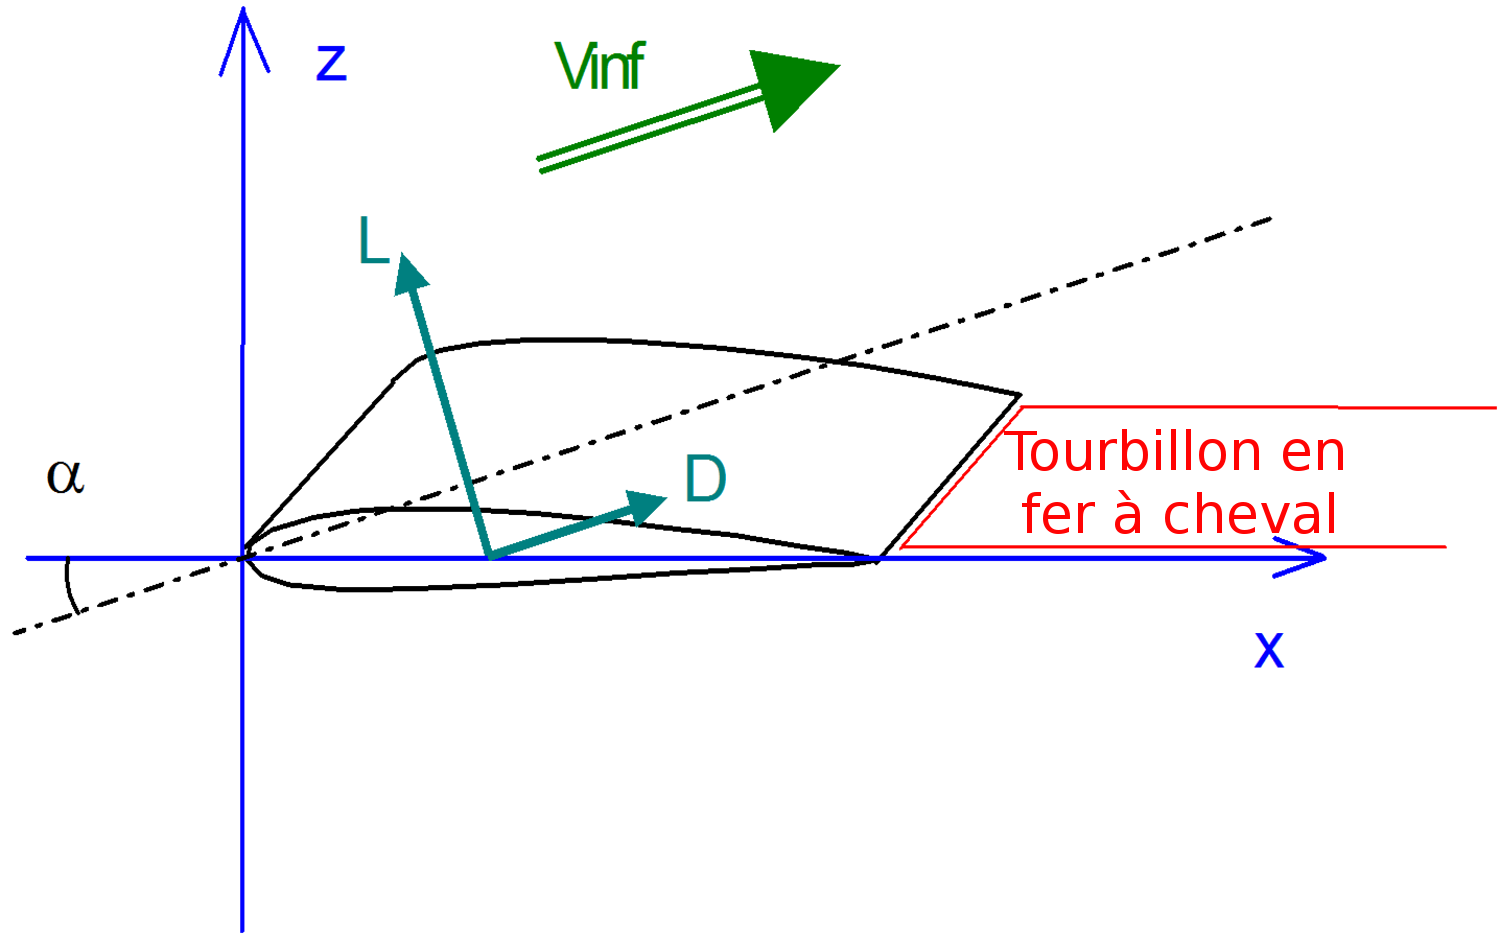
\includegraphics[width=0.7\linewidth]{img-29-fr}\centering\\
	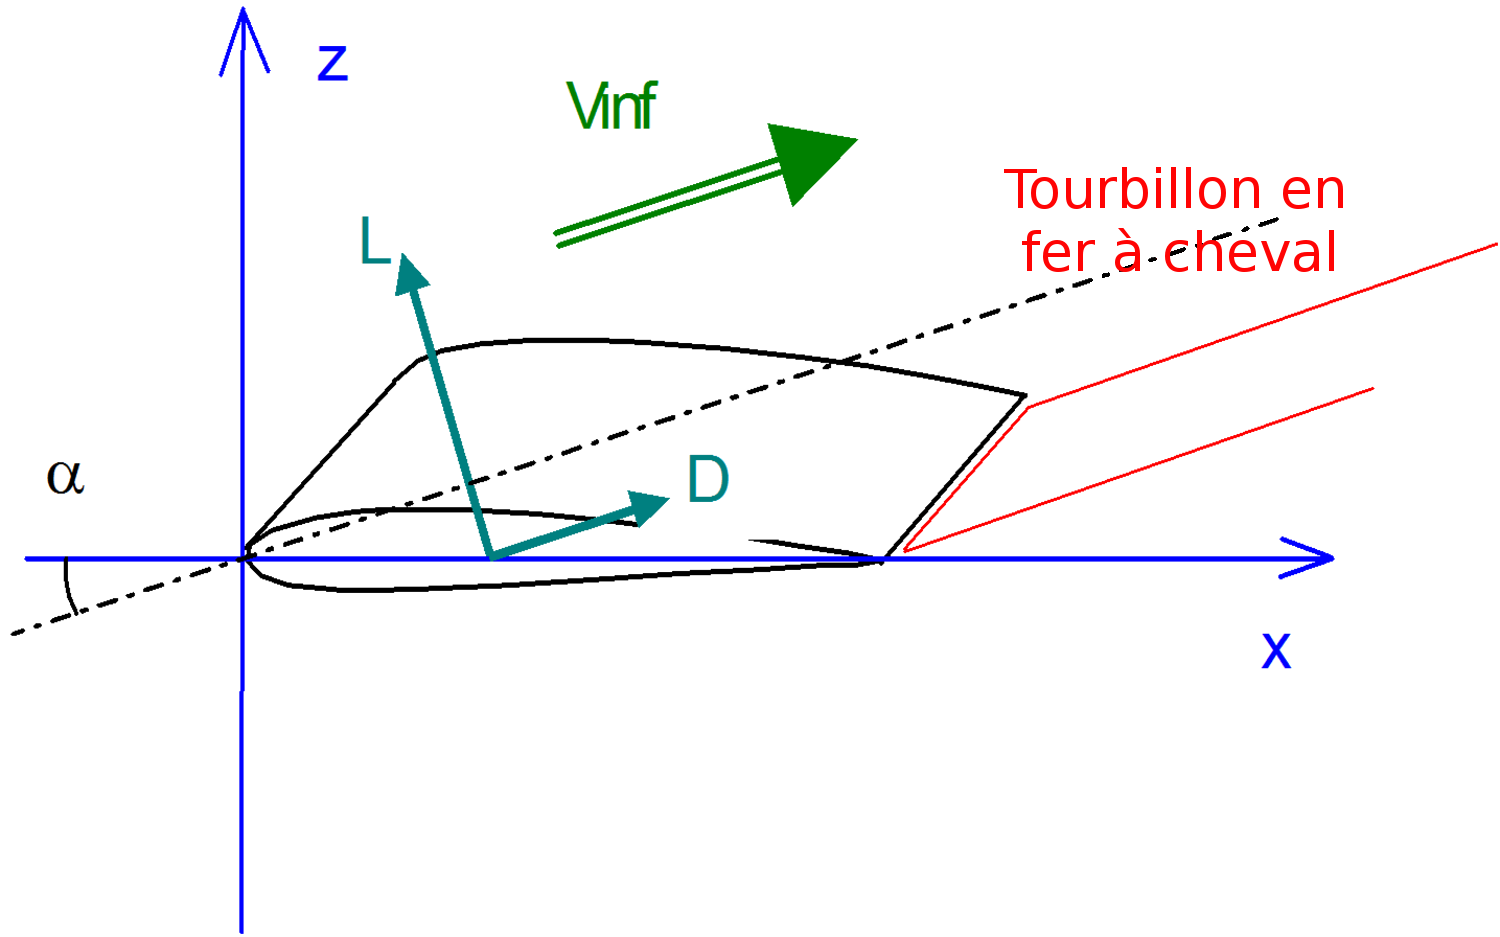
\includegraphics[width=0.7\linewidth]{img-30-fr}\centering\\
	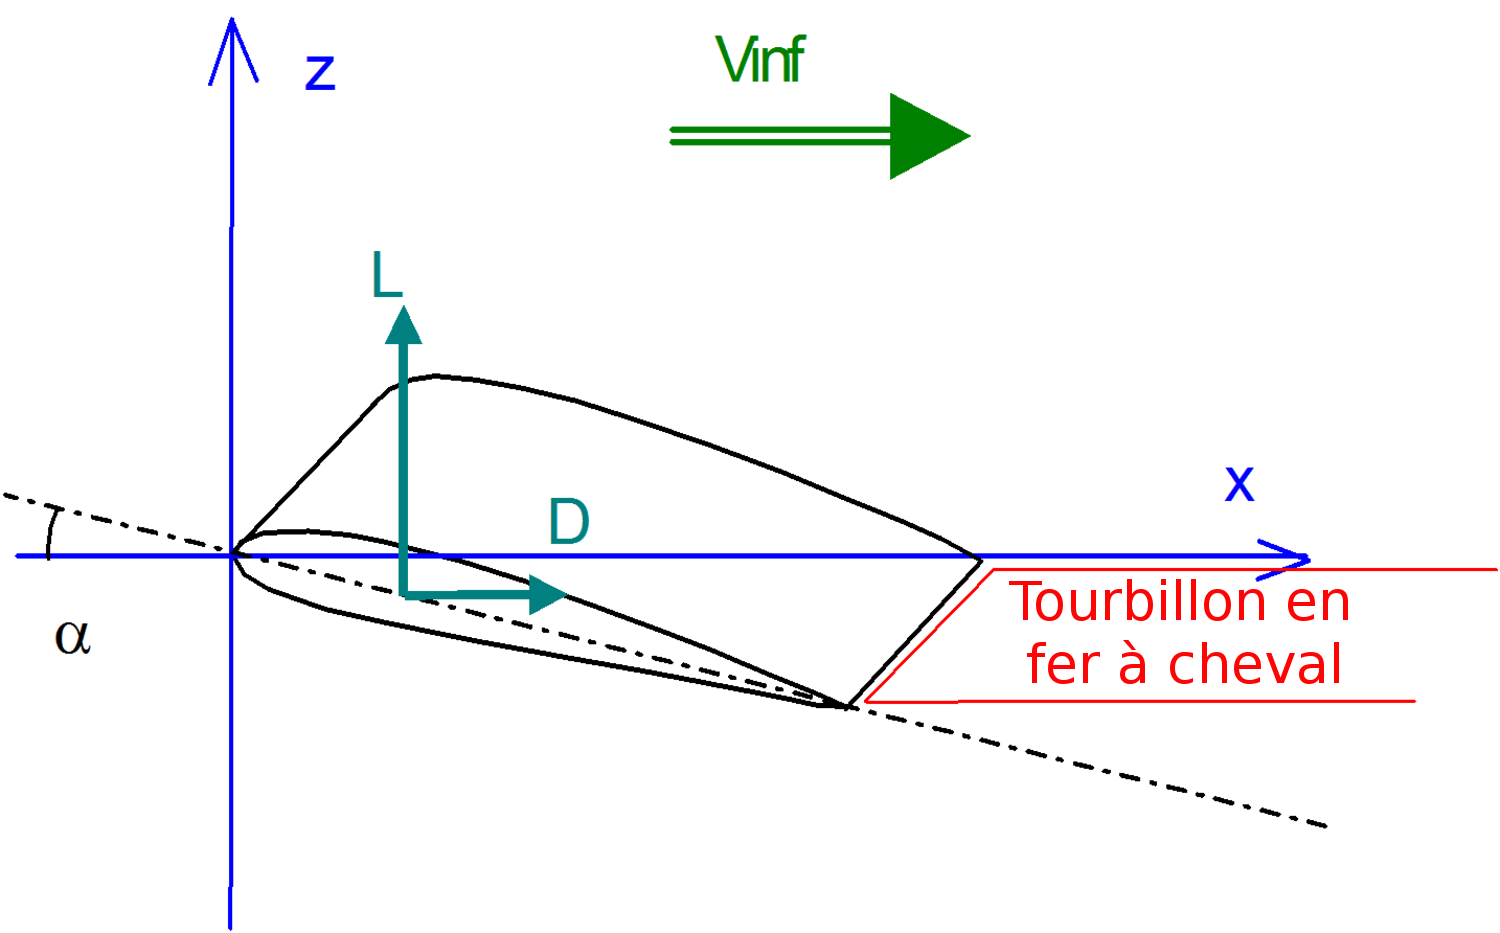
\includegraphics[width=0.7\linewidth]{img-31-fr}\centering
	\caption{Configuration de géométrie normale et inclinée}
	\label{img:configuration_géométrie_normale_inclinée}
\end{figure}

\clearpage
\paragraph{Enroulement du sillage – Analyse VLM et panneaux 3D}

\underline{Note}~: parce que c’est quelque chose sensible et difficile à utiliser, le processus d’enroulement de sillage a été désactivé. Les explications qui suivent ne sont fournies qu’à titre d’information.

\subparagraph{Considérations générales}

Dans leur formulation de base, les méthodes VLM et par panneaux font toutes
les deux l’hypothèse que le sillage est plat, ce qui est une approximation. 
Le sillage tend à s’enrouler sur lui-même, ce qui peut être illustré, par 
exemple par les deux tourbillons aux extrémités de chaque aile. Un modèle de sillage plus fin que la simple ligne droite ou le simple panneau plat peut être intéressant pour deux raisons~:

\begin{itemize}
	\item bien que le sillage ne porte pas de charge et n’a donc pas d’influence 
	sur le coefficient de portance, sa forme affecte la valeur de la traînée 
	induite et les coefficients dérivés~;
	\item un sillage plat n’est pas approprié à un avion comportant un 
	stabilisateur horizontal, car la déflexion de l’air dirigée vers le bas 
	créée par l’aile principale influe le champ d’écoulement autour du stabilisateur.
\end{itemize}

La forme du sillage est déterminée par le champ d’écoulement derrière l’aile, et à son tour, le champ d’écoulement dépend de la forme du sillage. La forme du sillage prise dans une situation d’état stable peut donc être déduite par un processus itératif dans lequel la géométrie du sillage est mise à jour («~relaxée~») après chaque boucle de calcul. 

\paragraph{Maillage du sillage}

La formulation des panneaux implémentée dans XFLR5 est de type panneau constant, plat. Il faut donc prêter une attention spéciale dans le choix de la taille du panneau de sillage afin d’éviter un vrillage excessif. La taille de panneau est contrôlée par trois paramètres~:

\begin{itemize}
  \item la longueur totale du sillage~;
  \item la dimension dans le sens de l’écoulement de la longueur du premier 
  panneau de sillage~;
  \item le rapport, ou facteur de progression, entre deux panneaux adjacents 
  dans la direction de l’écoulement.
\end{itemize}

Une indication générale est qu’il est conseillé de définir ces paramètres de manière à ce que la taille du premier panneau soit approximativement la même que celle du panneau de bord de fuite de l’aile. 

\paragraph{Processus d’enroulement}

Idéalement, les coefficients de portance et de traînée tendent vers des valeurs limites. Cependant, si aucune précaution spéciale n’est prise, les essais numériques montrent que le sillage tend à s’enrouler indéfiniment sur lui-même. Ceci conduit à des panneaux très vrillés et à une divergence numérique.

Comme l’enroulement n’est pas un processus robuste, les itérations sont 
limitées à la fois par le nombre d’itérations et par un critère de précision.
\begin{center}
\begin{tikzpicture}
	\tikzstyle{debutfin}=[ellipse,draw,text=red]
	\tikzstyle{instruct}=[rectangle,draw=black, fill=yellow!50, text 
	width=6cm,text centered]
	\tikzstyle{test}=[diamond, aspect=2.75,thick, draw=black, 
	fill=yellow!50,text=black, text width=7cm, text centered]
	\tikzstyle{es}=[rectangle,draw,rounded corners=4pt,fill=blue!25]

	\node[instruct] (a1) at (-2,20) {Définir la géométrie de sillage plat
	initial};
	\node[instruct] (a2) at (-2,18) {Configurer le problème pour la géométrie
	actuelle du sillage};
	\node[instruct] (a3) at (-2,16) {Résoudre le problème pour les valeurs de
	$\Gamma$ ou $\mu$ et $\sigma$};
	\node[test] (test) at (-2,12.75) {Reboucler jusqu’à ce que le nombre maximum
	d’itérations soit atteint};
	\node[instruct] (a5) at (-2,9.5) {Calculer les coefficients de l’OVNI};

	\tikzstyle{suite}=[->,>=stealth,thick,rounded corners=4pt]	

	\draw[suite] (a1) -- (a2);
	\draw[suite] (a2) -- (a3);
	\draw[suite] (a3) -- (test);
	\draw[suite] (test) -- (a5);
	
	\draw[suite] (test) -| (4,14.5) |- (-1,19) -- (a2);
\end{tikzpicture}
%	\caption{Implémentation de la LLT}
  \label{diagramme : itérations sillage}
\end{center}

La référence \cite{Werner} donne une description globale des problèmes 
liés à l’enroulement du sillage. 

\clearpage

\subsubsection{Moments}
\label{section : moments}

Tous les calculs de moments dans la LLT sont strictement en accord avec la formule de NACA TN1269.

Dans la version V4.00, la définition des moments a été modifiée pour clarifier certaines ambiguïtés qui existaient jusqu’à la version v3.21.

Depuis la version V4.00, les moments géométriques de tangage, roulis et lacet sont calculés par intégration des forces sur les panneaux. Pour VLM, ceci est réalisé à la position centrale du tourbillon, pour l’analyse par panneaux 3D, la force est appliquée au centre du panneau.

Les moments géométriques sont donc le total des moments appliqués à l’aile ou à l’avion. 

Dans un but d’analyse, il peut être intéressant de séparer ces moments en plusieurs parties, ou d’isoler une contribution spécifique au moment total. 

\underline{Bande de coefficients de moment}

Ces moments sont calculés pour chaque position sur l’envergure de l’aile et sont accessibles sur les graphes de point de fonctionnement.

\begin{table}[htbp]\scriptsize
	\centering
	\begin{tabular}{|*{4}{m{0.04\linewidth}|}*{3}{m{0.19\linewidth}|}}
	\hline
	\multicolumn{2}{|c|}{Moment} & Signe & Long.\newline Réf. & Nature &
    LLT &
    VLM \& Panneaux 3D\\
    \hline
    \multirow{2}{0.03\linewidth}{\begin{sideways}Tangage\end{sideways}} & 
    \begin{sideways}$Cm$~profil - Profil\end{sideways} & 
    \multirow{2}{0.03\linewidth}{\begin{sideways}positif nez haut\end{sideways}}
    & 
    \multirow{2}{0.03\linewidth}{\begin{sideways}C.A.M : $M=q.S.amc.Cm$
    \end{sideways}} & 
    Moment des forces de portance autour du point à 1/4 de la corde &
    La valeur du moment de cabrage est interpolée sur la polaire du maillage du
    profil. Elle prend en compte les effets visqueux &
    Somme des moments créés par les forces de pression sur la bande de panneaux.
    La part visqueuse est ignorée \\
    \cline{2-2} \cline{5-7}
    &
    \begin{sideways}$Cm$\end{sideways} &
    &
    &
    Moment des forces de pression et visqueuse par rapport à XCmRef &
    Intégration sur la ligne de portance de l’aile du moments des bandes 
    d’autocabrage, et de la force de portance de la bande. La flèche et le 
    dièdre sont tous les deux pris en compte &
    Somme sur tous les panneaux des moments des forces de pression + moment
    de tangage des forces de traînée visqueuse \\
    \hline
  \end{tabular}
  \caption{Coefficient des moment des bandes}
  \label{tablea : coefficient moments bandes}
\end{table}

\clearpage

\underline{Coefficients de moment de l’aile}

\begin{table}[H]\scriptsize
  \centering
  \begin{tabular}{|*{4}{m{0.04\linewidth}|}*{3}{m{0.19\linewidth}|}}
    \hline
    \multicolumn{2}{|c|}{Moment} &
    Signe &
    Long.\newline Réf. &
    Nature &
    LLT &
    VLM \& Panneaux 3D\\
    \hline % 8<---------------------

    \multirow{3}{0.03\linewidth}
    	{\begin{sideways}Tangage\end{sideways}} & 
%	    \begin{sideways}$GCm$ profil géom (global)\end{sideways} & 
	\begin{sideways}
		\parbox[t]{3cm}{$GCm$ profil géom \\ (global)}
	\end{sideways} &
    \multirow{3}{0.03\linewidth}
    	{\begin{sideways}positif nez haut\end{sideways}} & 
    
    \multirow{3}{0.03\linewidth}
    	{\begin{sideways}C.A.M~: $M=q.S.cam.Cm$ \end{sideways}} & 
    	
    Moment  par rapport à XCmRef des forces de pression &
    Intégration du moment sur la ligne portante de l’aile. La flèche et le 
    dièdre sont tous deux pris en compte &
    Somme sur tous les panneaux des moments des forces de pression\\

    \cline{2-2} \cline{5-7}
    &
%    \begin{sideways}$VCm$ visqueuse (global)\end{sideways} &
	\begin{sideways}
		\parbox[t]{2.5cm}{$VCm$ visqueuse \\ (global)}
	\end{sideways} &
    &
    &
    Moment par rapport à XCmRef des forces de traînée visqueuse du profil &
    \multicolumn{2}{|c|}
    	{Intégration du moment sur la ligne portante de l’aile.} \\
    \cline{2-2} \cline{5-7}
    &
    \begin{sideways}
    	\parbox[t]{4cm}{Profil (à la pos. locale sur l’env.)}
	\end{sideways} &
    &
    &
    Moment des forces de portance aux alentours de 1/4 de la corde&
    $Cm$ interpolé sur le maillage polaire 1&
    Somme des moments créés par les forces de pression sur les panneaux des
    bandes \\
    \hline % 8<---------------------
    \begin{sideways}Roulis\end{sideways} & 
    \begin{sideways}
    	\parbox{5cm}{\begin{center}{$GRm$ géom (global)}\end{center}}
	\end{sideways} &
	
%    \begin{sideways}$GRm$ géom (global)\end{sideways} & 

    \begin{sideways}positif avec l’aile tribord vers le bas\end{sideways} &
    \begin{sideways}Envergure~: $R=q.S.b.Cr$\end{sideways} & 
    Moment des force de pression par rapport à XCmRef &
    Intégration du moment de portance sur la ligne portante de l’aile. Le dièdre
    n’est pas pris en compte &
    Somme sur tous les panneaux des moments des forces de pression \\
    \hline % 8<---------------------

    \multirow{3}{*}{\begin{sideways}Lacet\end{sideways}} & 
%    \begin{sideways}$GYm$ géom (global)\end{sideways} & 
    \begin{sideways}
    	\parbox[t]{2cm}{$GYm$ géom \\ (global)}
	\end{sideways} &


    \multirow{3}{4cm}{\begin{sideways}positif avec le nez à
    tribord\end{sideways}} & 

    \multirow{3}{0.03\linewidth}{\begin{sideways}Envergure~:
    $N=q.S.b.C_n$\end{sideways}} & 
    Moment des force de pression par rapport à XCmRef &
    N/D&
    Somme sur tous les panneaux des moments de fotces de pression\\
    \cline{2-2} \cline{5-7}
    &
%    \begin{sideways}$VYm$ profil (global)\end{sideways} &
    \begin{sideways}
    	\parbox[t]{2cm}{$VYm$ profil\\ (global)}
	\end{sideways} &
    &
    &
    Moment des force de pression visqueuses du profil par rapport au plan y=0 &
    \multicolumn{2}{|c|}{Intégration du moment sur la ligne portante de
    l’aile} \\
    \cline{2-2} \cline{5-7}
    &
%    \begin{sideways}$IYm$ induit (global)\end{sideways} &
	\begin{sideways}
    	\parbox[t]{2cm}{$IYm$ induit \\ (global)}
	\end{sideways} &
    &
    &
    Moment des forces tangentielles induites par rapport au plan y=0 &
    \multicolumn{2}{|c|}{Intégration du moment sur la ligne portante de l’aile}\\
    \hline % 8<---------------------
  \end{tabular}
  \caption{Coefficient de moment de l’aile}
  \label{tab:wing_moment_coefficients}
\end{table}

\clearpage
\subsubsection{Point neutre, centre de pression, marge statique}

XFLR5, jusqu’à sa version v3.12, a fourni une mesure de la quantité 
$$SM~=~\frac {(X_{CP} - X_{CG})} {CAM} $$
incorrectement marquée «~Marge statique~», où~:

\begin{tabular}{rl}
	$X_{CP}$ & est la position le long de la ligne de flux du centre de 
	pression\\
	$X_{CG}$ & est la position le long de la ligne de flux du centre de gravité
\end{tabular} 

La marge statique conventionnelle d’une aile ou d’un avion devrait être déterminée par un processus itératif. C’est la position du centre de gravité (ou
la position de référence du moment $XCmRef$) pour laquelle 

$$\frac {dCm} {d\alpha} = 0$$
Ceci est illustré sur la figure Figure~\ref{img:point_neutre_aile}
où le point neutre est approximativement à 67~mm du bord d’attaque. 

\begin{figure}[htbp]
	\centering
	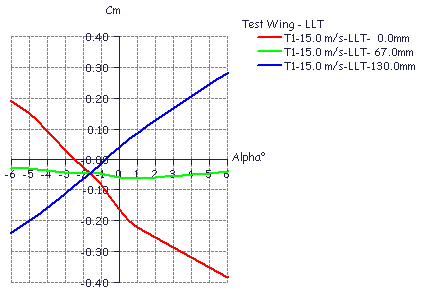
\includegraphics[width=0.8\linewidth]{img-33}
	\caption{Point neutre de l’aile}
	\label{img:point_neutre_aile}
\end{figure}

L’illustration sur la manière d’utiliser XFLR5 pour placer le CG d’un modèle est donnée dans \cite{DeperroisStab} et \cite{DeperroisNotions}.

\clearpage

\subsubsection{Facteur d’efficacité}
Le facteur d’efficacité, encore appelé facteur d’Oswald est une mesure des 
déplacements de la traînée induite de l’aile par rapport à une charge optimale 
elliptique. Il est défini par
$$e~=~\frac{Cz^2} {\pi \cdot AR \cdot ICx}$$

où~:

\begin{tabular}{rl}
	$Cz$ & est le coefficient de portance\\
	$ICx$ & est le coefficient de traînée induite\\
	AR & est l’allongement de l’aile
\end{tabular}

Le facteur d’efficacité, encore appelé facteur d’Oswald devrait toujours être inférieur à 1. Il arrive cependant que ce facteur devienne supérieur à 1 pour des raisons numériques dans les calculs de LLT, VLM et de panneaux 3D. 

En LLT, ceci peut être corrigé en augmentant la précision exigée pour la convergence, par exemple avec les paramètres suivants~:

\begin{tabular}{r@{\ =\ }l}
	Nombre de points d’interpolation & 40\\
	Facteur de relaxation & 40\\
	Critère de convergence & 0.001\\
	Nombre maximum d’itérations & 300
\end{tabular}

En VLM et panneaux 3D, une amélioration de la densité des panneaux sans la 
direction du flux est nécessaire pour réduite le facteur d’efficacité à des 
valeurs inférieures à 1. 

\subsubsection{Points de fonctionnement de l’aile et polaires de l’aile}
La présentation des résultats est la même que pour l’analyse d’un profil, c’est-à-dire que que analyse ayant convergé génère un point de fonctionnement et ajoute un résultat à l’objet polaire. La définition et la sélection d’un objet Analyse/Polaire est nécessaire pour pouvoir effectuer un calcul.

 
Un nombre quelconque de points de fonctionnement peut être enregistré dans 
la base de données créée au moment de l’exécution, la seule limite est celle de la mémoire de l’ordinateur. Les points de fonctionnement de l’aile et de l’avion utiliseront des ressources mémoires conséquentes.

Les polaires de Type 1 et de Type 4 demeurent inchangées par rapport à l’analyse de profil.

Une polaire de Type 2 correspond à un avion d’une masse donnée fonctionnant à portance constante.

Pour un angle d’attaque donné, la vitesse de l’avion est calculée pour créer une
force de portance opposée au poids de l’avion~: 
$$V~=~\sqrt{\frac{2\cdot mg}{\rho SCz}}$$

L’angle de descente est~:
$$\gamma~=~\arctan \left(\frac{Cx}{Cz}\right)$$

et les vitesses horizontale et verticale sont respectivement~:
$$ V_x = V_\infty \cos(\gamma) $$
$$ V_z = V_\infty \sin(\gamma) $$

\begin{figure}[htbp]
  \centering
  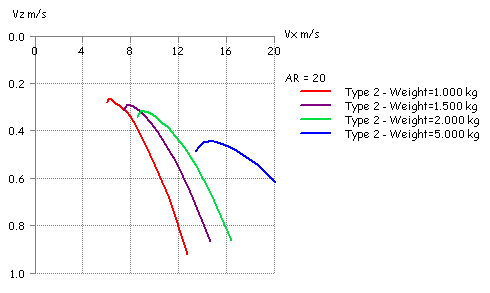
\includegraphics[width=0.8\linewidth]{img-34}
  \caption{Polaires de vitesse basées sur une analyse de Type 2}
  \label{img:polaire_vitesse_analyse_type_2}
\end{figure}

La convergence pour les polaires de type 2 exige que l’angle d’attaque 
apparent soit supérieur à l’angle de portance nulle. Sinon aucune vitesse
ne pourra générer de portance positive\dots

\subsubsection{Analyse de contrôle – Polaire de Type~5 et de Type~6}

Les polaires de contrôle de Type~5 et de Type~6 ont été désactivées dans
XFLR5~v6 et ont été remplacées par les polaires de stabilité de Type~7.

\subsubsection{Interpolation du maillage polaire généré par XFoil}
Le code ne recalcule pas avec XFoil chaque point de fonctionnement à chaque 
position sur l’aile et pour chaque itération~: 
\begin{itemize}
	\item ceci donnerait des temps de calcul exagérément – et inutilement – 
	longs~;
	\item la convergence de XFoil est trop incertaine.
\end{itemize}

En remplacement, le point de fonctionnement est interpolé depuis un jeu 
pré-généré de polaires de Type 1.

Les calculs de l’aile exigent que ce jeu de polaires de profil de \textbf{Type 1} soit préalablement chargé ou généré pour chacun des profils de l’aile.

\begin{figure}[H]
	\centering
	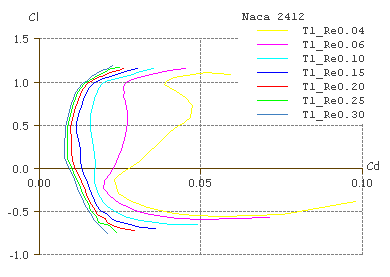
\includegraphics[width=0.8\linewidth]{img-35}
	\caption{Maillage polaire s’étendant de $Re = 40~000$ to $Re = 300~000$}
	\label{img:plage_maillage_polaire}
\end{figure}

Le jeu de polaires devrait couvrir l’ensemble du domaine de vol en chaque 
point de l’aile pour, à la fois le nombre de Reynolds et l’angle d’attaque
apparent.

Si un point quelconque de la forme développée de l’aile fonctionne hors du 
maillage polaire disponible, un message d’avertissement sera émis dans le 
fichier journal. Ceci se produit, par exemple, dans le cas des cordes
d’extrémités courtes des ailes elliptiques. Dans un tel cas, le point du
maillage «~le plus proche~» sera utilisé, et le point de fonctionnement
pourra être généré et ajouté à la polaire en cours, si l’utilisateur l’a
choisi ainsi.

Pour le processus d’interpolation, le code utilise indifféremment toutes
les polaires de Type 1 disponibles et qui concernent le profil sélectionné.
L’utilisateur doit donc faire attention de ne fournir qu’un jeu de polaires
homogène et cohérent.

Le processus d’interpolation d’une variable $X$ ($X$ pouvant être $Cz, Cx, Cm$, les points de transition, etc.) depuis $[\alpha = aoa\footnote{aoa = Angle Of Attack, il s’agit de l’angle d’attaque.} + \alpha_i + washout, Re]$ à un point géométrique $P$ entre les profils 1 et 2 est~:

\begin{enumerate}
	\item Pour le premier profil, rechercher les polaires 1 et 2 telles que
	$Re_1 < Re < Re_2$
	\begin{itemize}[label=]
		\item si ni la polaire 1, ni la 2 ne sont trouvées, retourner une erreur
		\item si $Re$ est inférieur aux nombres de Reynolds de toutes les 
		polaires, utiliser la polaire ayant le $Re$ le plus faible
		\item si $Re$ est supérieur à celui de toutes les polaires, utiliser la
		polaire ayant le $Re$ le plus grand. 
	\end{itemize}
	\item Interpoler chaque polaire avec $\alpha$ pour obtenir $X_{11}$ et
	$X_{12}$.

	\begin{itemize}[label=]
	    \item si aucune polaire n’est définie jusqu’à $\alpha$, utiliser le plus 
	    petit ou le plus grand angle disponible et émettre un avertissement.
	    \item si une seule polaire est disponible, n’interpoler que cette 
	    polaire et émettre un avertissement.
	\end{itemize}
	\item Interpoler $X_1$ entre $X_{11}$ et $X_{12}$, au prorata de $Re$ entre 
	$Re_1$ et $Re_2$.
	\item Effectuer la même chose avec le second profil pour obtenir $X_2$.
	\item Interpoler $X$ entre $X_1$ et $X_2$, au prorata de la position du 
	point entre les deux profils.
\end{enumerate}

\subsubsection{Lignes de courant}
Les lignes de courant sont calculées à partir des l’intensité des tourbillons, ou des intensités dipôles et sources, chaque fois qu’un point de fonctionnement
est sélectionné.

Les calculs sont incrémentaux, dans la direction x du flux.

Les lignes de courant commence au bord d’attaque ou de bord de fuite des panneaux du maillage, avec un décalage dans les directions x et z défini par l’utilisateur.

La «~longueur initiale~» est le premier incrément en x pour les calculs de la ligne de courant.

Le «~facteur d’avancement~» détermine la longueur du pas $n+1$ relativement au pas $n$.

Note d’avertissement~: le vecteur-vitesse est singulier aux arêtes des panneaux dans l’analyse par panneaux 3D, et sur la ligne de traînée des tourbillons des panneaux dans l’analyse VLM. Ceci peut entraîner des instabilités numériques, dans le cas où, par exemple, on demande aux lignes de courants de commencer exactement au bord de fuite ou au bord  d’attaque des panneaux, ou aux coins d’un panneau. Un léger décalage en x ou z est nécessaire pour éviter l’instabilité. L’utilisation d’un rayon de noyau de tourbillon, qui peut être défini dans les paramètres avancés, est une autre possibilité.

\subsubsection{Comparaison avec les résultats expérimentaux}
Le code a été testé par comparaison avec des résultats expérimentaux et par 
comparaison avec d’autres logiciels, avec des résultats cohérents.

De plus, les algorithmes VLM, panneaux 3D et LLT dans leur implémentation
dans XFLR5 sont totalement indépendants, mais ils donnent des résultats
proches dans la partie linéaire des diagrammes de $Cz$ en fonction de $\alpha$.

\begin{figure}[htbp]
  \centering
  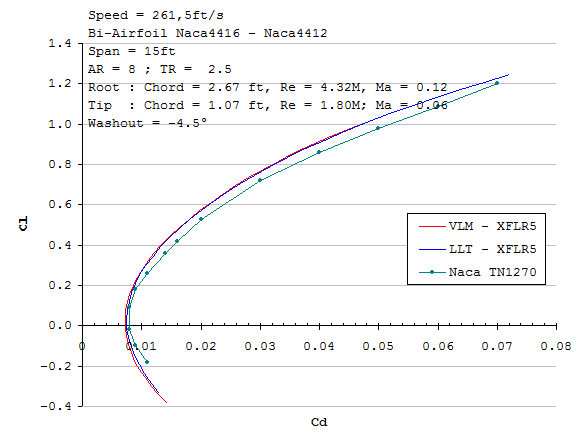
\includegraphics[width=0.8\linewidth]{img-36}
  \caption{Comparaison avec les résultats de test de Naca Tech. Note 1270}
  \label{img:comparaison_réesultats_tests}
\end{figure}

\subsubsection{Comparaison avec des données de soufflerie}

Une expérience a été menée début 2008 avec un modèle réduit de planeur. Les 
résultats détaillés sont donnés en \cite{DeperroisResults}. 

Les figures suivantes donnent les résultats de XFLR5 v3.21 et v4.09. Les 
résultats de v3.21 sont marqués «~FMe~» parce que les calculs ont été
réalisés par F. Meschia.

Note~: en v4.09, les calculs de portance ont été effectués par intégration 
des forces de pression sur les panneaux. Depuis v4.13, les calculs sont
réalisés dans le plan du champ lointain. 

\begin{figure}[htbp]
  \centering
  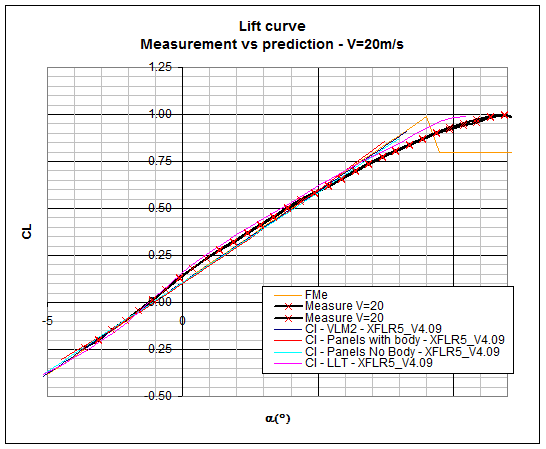
\includegraphics[width=0.8\linewidth]{img-37}
  \caption{Courbe de portance prédite par rapport aux résultats expérimentaux}
  \label{img:courbe_portance_prédite_résultats_expérimentaux}
\end{figure}

\begin{figure}[htbp]
  \centering 
  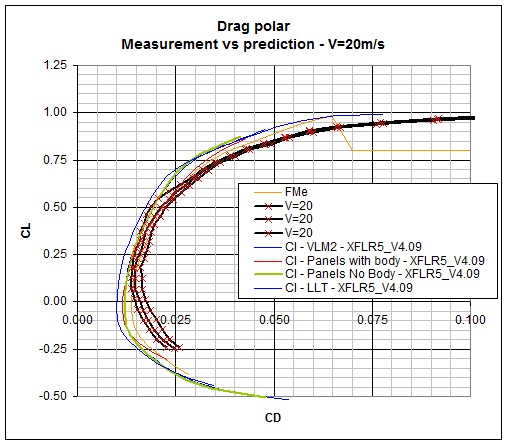
\includegraphics[width=0.8\linewidth]{img-38}
  \caption{Polaire de traînée prédite par rapport aux résultats expérimentaux}
  \label{img:polaire_traînée_prédite_résultats_expérimentaux}
\end{figure}

\begin{figure}[htbp]
  \centering 
  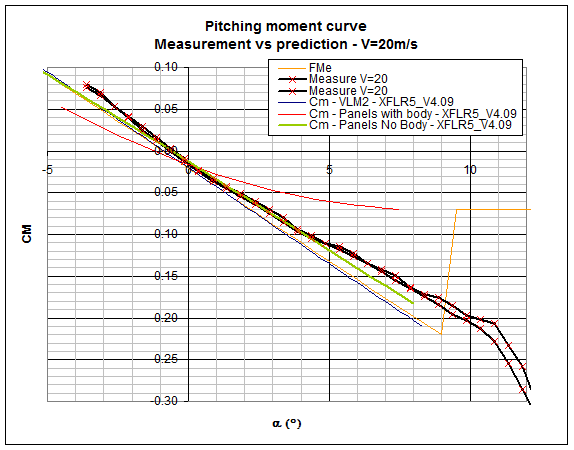
\includegraphics[width=0.8\linewidth]{img-39}
  \caption{Moment de cabrage prédit par rapport aux résultats expérimentaux}
  \label{img:moment_cabrage_prédit_résultats_expérimentaux}
\end{figure}

\pagebreak

On peut en conclure que~:

\begin{itemize}
  \item la VLM est au moins aussi fiable que la méthode des panneaux 3D~;
  \item la modélisation du fuselage n’améliore pas la précision des
  résultats~;
  \item les deux méthodes donnent une estimation raisonnable de valeurs
  telles que~:
  \begin{itemize}
    \item coefficient de portance~;
    \item angle à portance nulle~;
    \item coefficient de moment de tangage~;
    \item moment de portance nulle ou portance à moment nul.
  \end{itemize}
  \item Les deux méthodes tendent à sous-estimer la traînée, probablement sa
  part visqueuse.
\end{itemize}

\subsubsection {Comparaison des résultats de Miarex et d’AVL}

\begin{figure}[!ht]
  \centering
  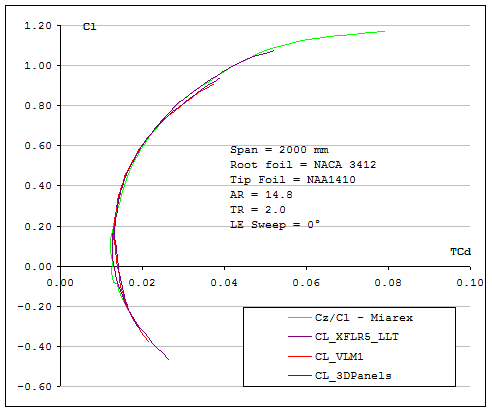
\includegraphics[width=0.8\linewidth]{img-40}
  \caption{Coefficient de portance – Comparaison des résultats de Miarex}
  \label{img:comparaison_AVL_miarex_coefficient_portance}
\end{figure}

\begin{figure}[!ht]
  \centering
  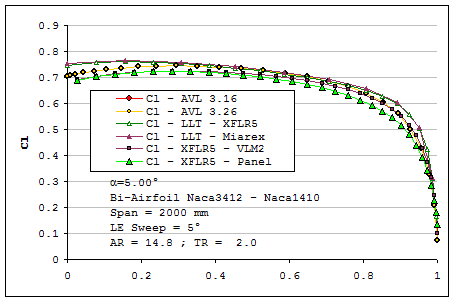
\includegraphics[width=0.8\linewidth]{img-41}
  \caption{Angle induit – Comparaison entre AVL et Miarex}
  \label{img:comparaison_AVL_miarex_angle_induit}
\end{figure}

\begin{figure}[!ht]
  \centering
  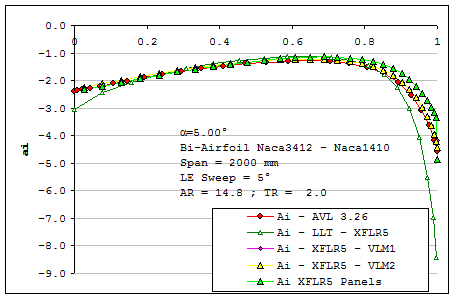
\includegraphics[width=0.8\linewidth]{img-42}
  \caption{Angle induit en fonction de l’envergure – Comparaison entre AVL et 
  Miarex}
  \label{img:comparaison_AVL_miarex_angle_induit_envergure}
\end{figure}

\begin{figure}[!ht]
  \centering
  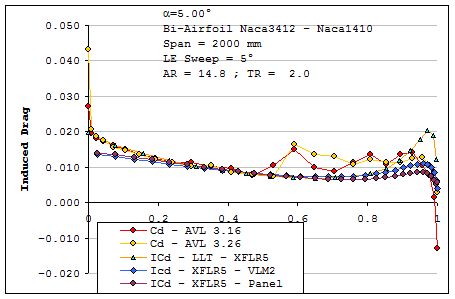
\includegraphics[width=0.75\linewidth]{img-43}
  \caption{Traînée induite en fonction de l’envergure – Comparaison entre AVL et 
  Miarex}
  \label{img:comparaison_AVL_miarex_traînée_induite_envergure}
\end{figure}

Note concernant la traînée induite~: l’hétérogénéité des résultats d’AVL 
est inexpliquée.

\begin{figure}[!ht]
  \centering
  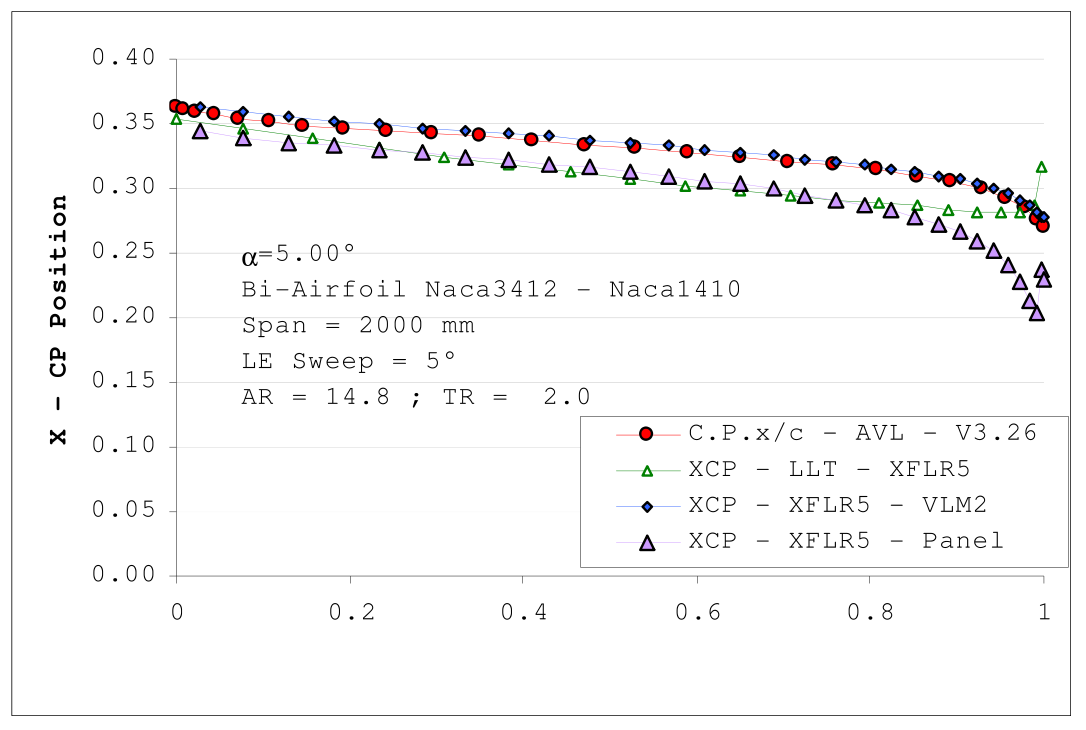
\includegraphics[width=0.75\linewidth]{img-44-fr} %073a
  \caption{Centre de pression en fonction de l’envergure – Comparaison entre AVL 
  et Miarex}
  \label{img:comparaison_AVL_miarex_centre_pression_envergure}
\end{figure}

\begin{figure}[!ht]
  \centering
  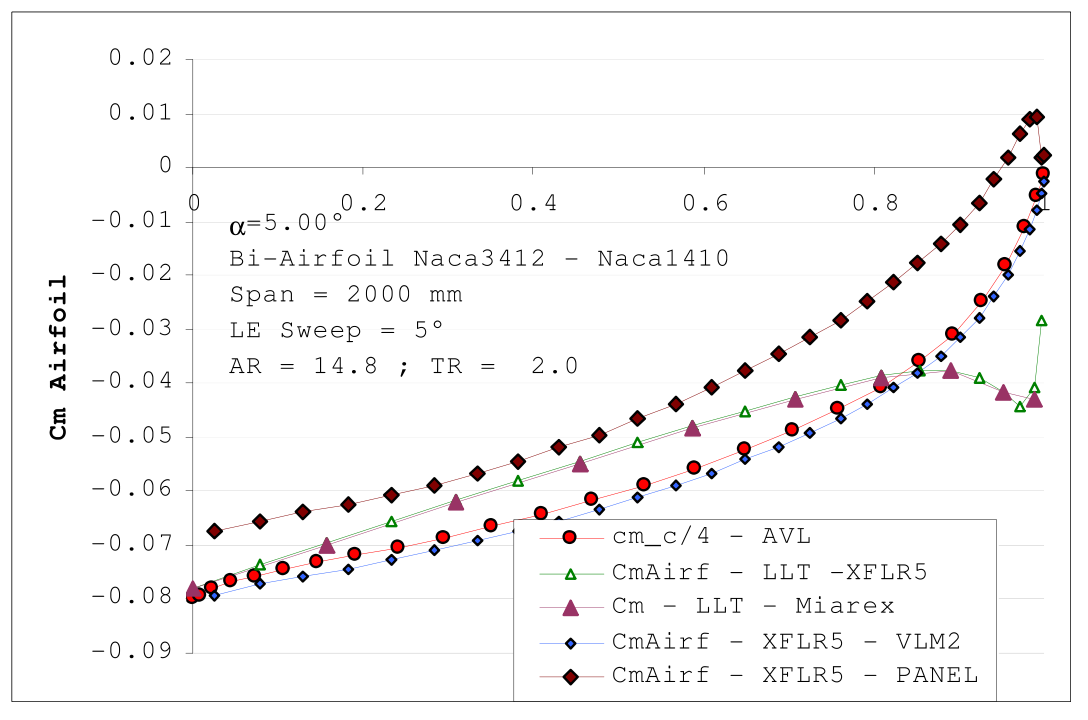
\includegraphics[width=0.75\linewidth]{img-45-fr} %075a
  \caption{Moment de tangage en fonction de l’envergure – Comparaison entre AVL
  et Miarex}
  \label{img:comparaison_AVL_miarex_moment_tangage_envergure}
\end{figure}

\clearpage

\subsubsection{Exemple de session – Analyse d’aile}
\label{section : exemple session analyse aile}

\begin{enumerate}
	\item Charger le(s) profil(s) qui seront utilisés pour définir l’aile~;
	\item Dans l’application d’analyse directe, cliquez «~Lancer l’analyse par 
	lots~» depuis le menu «~Analyse~», ou pressez \touche{Maj}+\touche{F6}~;
	\item Lancer une analyse par lots avec les paramètres suivants (assurez-vous 
	que les valeurs couvrent l’ensemble du domaine de vol de l’aile)~:
	\begin{itemize}
		\item avec $\alpha = -6\degree$ à $\alpha = 10\degree$~;
		\item avec $Re = 40~000$ à $Re = 160~000$ tous les $20~000$~;
		\item avec $Re = 200~000$ à $Re = 500~000$ tous les $50~000$
	\end{itemize}
	ou utilisez une liste prédéfinie.\\
	Cocher la case «~Depuis zéro~» fera démarrer l’analyse depuis $\varpi =
	0\degree$ en augmentant jusqu’à $\alpha_{max}$ et en redescendant ensuite à
	$\alpha_{min}$~; ceci facilite en général la convergence~;
	\item Fermer la boîte de dialogue~;
	\item Optionnel~: utiliser «~Enregistrer les polaires associées~» dans le
	menu «~Profil actuel~» afin d’enregistrer les polaires dans un fichier
	«~.plr~» pour les utiliser dans de futurs projets~;
	\item Aller à l’application de conception d’aile en pressant \touche{Ctrl}+
	\touche{6}~;
	\item Cliquer la commande «~Définir une aile~» ou pressez \touche{F3} depuis
	le menu Aile, ou «~Définir un avion~» (\touche{Ctrl}+\touche{F3})~;
	\item Définir l’objet et fermer la boîte de dialogue~;
	\item Optionnel mais recommandé~: définir les propriétés d’inertie de 
	l’objet actuel avion ou aile~;
	\item Sélectionner l’avion actuel (ou l’aile)/Définir l’inertie~;
	\item Entrer les propriétés d’inertie pour l’avion ou l’aile~;
	\item Assurez-vous que la position du centre de gravité est située où elle
	est supposée être. Il peut être nécessaire de «~tricher~» un peu sur la
	position des masses ponctuelles pour obtenir la position désirée~;
	\item Fermer la boîte de dialogue~;
	\item Cliquer «~Définir une Analyse/Polaire~» depuis le menu Polaire d’aile
	ou presser \touche{F6}~;
	\item Activer la coche «~Type 2~»~;
	\item Définir la masse de l’avion et la position du centre de gravité 
	(l’emplacement de la référence de moment) ou sélectionner l’option 
	d’utiliser l’inertie de l’avion~;
	\item Sauf si l’aile à un faible allongement, une forte flèche ou un dièdre
	important, sélectionnez la case à cocher «~LLT~» et fermez la boîte de 
	dialogue (presser deux fois \touche{Entrée}~;
	\item Laisser les paramètres de LLT à leurs valeurs par défaut dans le menu
	 «~Point de fonctionnement~», c’est-à-dire «~Facteur de relaxation = 20~» et
	 «~Nb de points d’interpolation le long de l’envergure = 20~» 
	 \item Sélectionner dans la barre d’outils de droite l’angle d’attaque qui
	 peut être supposé donner une portance positive supérieure au poids de 
	 l’avion à des valeurs raisonnables de Vitesse/Re – par exemple $\alpha = 
	 3\degree$;
	\item Cliquer le bouton \bouton{Analyser} dans la barre d’outils de droite~;
	\item Changer les paramètres si l’on n’atteint pas de convergence de la
	LLT ou continuer l’analyse LLT après avoir décoché la case «~Init LLT~»
	\item Cliquer la commande «~Vue 3D~» depuis le menu Afficher~;
	\item Utiliser la souris pour zoomer et pivoter le modèle~;
	\item Cocher «~Séquence~» pour calculer la polaire complète de l’aile~;
	\item Cliquer la commande «~Polaires~» du menu Afficher ou presser
	\touche{F8} pour visualiser les diagrammes polaires.
\end{enumerate}

\subsubsection{Non convergences}

\begin{table}[htbp]\scriptsize
  \centering
  \begin{tabular}{|m{0.18\linewidth}|m{0.38\linewidth}|m{0.38\linewidth}|}
    \hline
    &
    Cause &
    Correction \\
    \hline
    \multirow{4}{0.18\linewidth}{Toutes méthodes} &
    Les maillages polaires de Type 1 du profil ne couvrent pas le domaine de
    vol disponible\newline
    (cas le plus courant de non convergence) &
    Étendre le maillage polaire de Type 1 des profils\\
    \cline{2-3}
    &
    En analyse de Type 2, la portance est négative & 
    Ne faire les calculs que pour des valeurs plus élevées de l’angle
    d’attaque\\
    \cline{2-3}
    &
    En analyse de Type 2, la vitesse est soit trop basse soit trop élevée,
    ce qui donne des points de fonctionnement en dehors du domaine de vol &
    Étendre le maillage polaire de Type 1 du profil~; La vitesse va tendre
    vers des valeurs infinies aux faibles angles d’attaque et, symétriquement
    elle va tendre vers 0 aux forts angles d’attaque\\
    \cline{2-3}
    &
    La corde d’extrémité est trop faible ce qui conduit à des nombres de 
    Reynolds trop faibles &
    Soit~:
    \begin{enumerate}
     \item Cocher la case «~Enregistrer les OpPoints en dehors du maillage
     polaire~»
     \item Supprimer l’extrémité de l’aile dans la définition de sa forme 
     développée
    \end{enumerate} \\
    \hline
    \multirow{2}{0.18\linewidth}{LLT} & 
    Le facteur de relaxation est trop faible &
    Augmentez le facteur dans la boîte de dialogue «~Paramètres de LLT\dots~»\\
    \cline{2-3}
    &
    Le nombre de points sur la forme développée est trop élevé &
    Diminuez le nombre dans la boîte de dialogue «~Paramètres de LLT\dots~»\\
    \hline
    VLM &
    La matrice est singulière en raison d’une disposition des panneaux VLM
    conflictuelle &
    Régénérez manuellement un maillage VLM \\
    \hline
    Panneaux &
    Les résultats sont incohérents parce que le sillage engendré par l’aile
    et la profondeur sont sur le même plan horizontal & 
    Décalez soit l’aile, soit le stabilisateur dans la direction z, de
    manière à ce qu’ils ne soient pas sur le même plan.\\
    \hline
  \end{tabular}
  \caption{Causes de non convergence et solutions}
  \label{table non convergences causes et solutions}
\end{table}

Le fichier journal indiquera quels sont les points du domaine de vol qui ne 
peuvent pas être calculés. On peut y accéder par la commande de menu «~Points
de fonctionnement / Afficher le fichier journal~»

Le «~fichier journal (log)~» est un fichier en texte pur. Si le document ne 
s’affiche pas lorsqu’il est appelé depuis le menu, il peut être nécessaire 
d’associer vous-même l’extension «~.log~» à un éditeur de texte de votre système.

\subsection{Analyse de stabilité et de contrôle}

Le but de l’analyse de stabilité et de contrôle est d’évaluer le temps de réponse d’un avion à une perturbation à partir d’une condition de vol stable. La perturbation peut provenir de l’environnement, par exemple une rafale de vent, ou l’action d’une commande.

La représentation mathématique de la réponse est quelque chose de complexe, qui demande quelques hypothèses simplificatrices. Principalement, seules les faibles perturbations depuis les conditions de vol stable seront prises en compte.

On trouvera l’aspect théorique de la dynamique du vol et de l’analyse de  stabilité dans la référence \cite{Sivells47}. Le but de ce document est de~:

\begin{itemize}
	\item fournir une courte description très simplifiée de la dynamique du vol
	pour les utilisateurs qui ne sont pas familiers avec la théorie~;
	\item expliquer les choix faits dans XFLR5~;
	\item et décrire la procédure d’analyse.
\end{itemize}

Note~: les concepts mathématiques et les formules présentés ci-après ne sont pas absolument nécessaires à la compréhension de la physique de la dynamique du vol. Ils sont fournis en tant qu’information et de base pour ceux qui sont intéressés à investiguer plus profondément les concepts.

\subsubsection{Méthode}

\subsubsection{Théorie}

XFLR5 suit la méthode proposé par Etkin dans la référence \cite{Etkin}.

Avec ce type d’analyse, les dynamiques latérale et longitudinales sont évaluées séparément.

\subsubsection{Repères de référence}

Trois repères de références différentes sont pris en considération pour l’analyse de la stabilité~: le repère géométrique, le fuselage, et le repère aérodynamiques. Ils sont définis sur la figure 
Figure~\ref{img:repères_fuselage_aérodynamique}.

\begin{figure}[htbp]
	\centering
	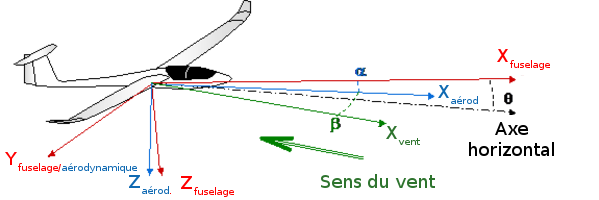
\includegraphics[width=0.8\linewidth]{img-46-fr}
	\caption{Repère de fuselage et aérodynamique}
	\label{img:repères_fuselage_aérodynamique}
\end{figure}

\underline{Repère du fuselage~:}

Le terme repère de fuselage est générique et se réfère à toute structure 
qui est fixée au fuselage, et ce n’est donc pas une structure d’inertie
ni de référence. Comme d’habitude, mais ce n’est pas universel, les
conventions sont les suivantes~:

\begin{itemize}
	\item l’axe X' est aligné avec le nez du fuselage~;
	\item l’axe Z' est dans le plan de symétrie, et est orienté vers le bas~;
	\item l’axe Y' est perpendiculaire au plan XY et est orienté vers tribord.
\end{itemize}

\underline{Repère géométrique~:}

C’est la structure de référence dans laquelle la géométrie est définie.

\begin{itemize}
	\item l’axe X est aligné «~à l’envers~»~;
	\item l’axe Z est dans le plan de symétrie, il est orienté vers le haut~;
	\item l’axe Y est perpendiculaire au plan xz, il est orienté vers tribord.
\end{itemize}

Le repère géométrique est un cas particulier de repère de fuselage.

\underline{Repère aérodynamique~:}

Il s’agit de la structure dans laquelle le mouvement dans des conditions
d’état stable est le mieux décrit~:

\begin{itemize}
	\item l’axe x est la projection du vecteur-vitesse sur le plan xy du
	fuselage~; cet axe est donc orienté vers l’avant~;
	\item l’axe z est orienté vers le bas~;
	\item l’axe y est orienté vers tribord.
\end{itemize}

Le point d’origine de la structure est le centre de gravité CG de l’avion.

Le repère aérodynamique sont un cas particulier de repère de fuselage.

\underline{Notes~:}

\begin{itemize}
	\item En vol horizontal, l’axe $X_{aérodynamique}$ est horizontal~;
	\item Comme le dérapage est simulé dans XFLR5 par une rotation de la 
	structure autour de l’axe d’inertie $Z_E$, le repère du vent est le même le
	repère aérodynamique, même si le dérapage n’est pas nul~;
	\item Dans les conditions d’équilibre, le repère aérodynamique est fixé au
	fuselage, et n’est donc pas un repère d’inertie.
\end{itemize}

XFLR5 suit la recommandation de \cite{Etkin} et effectue tous les
calculs dans le repère aérodynamique.

\subsubsection{Coordonnées, position, vecteurs vitesse et rotation}

La position du fuselage dans le repère aérodynamique est définie dans une
certaine structure d’inertie de référence par la position de son origine
O(x,y,z), et par la rotation définie par les angles d’Euler 
(\textrm{${\varphi}$, ${\theta}$,${\psi}$}).

Supposons que V(U,V,W) soit le vecteur-vitesse du fuselage, et supposons
que \textrm{${\omega}$}(P,Q,R) soit le vecteur-rotation du fuselage, les
deux étant définis dans le repère aérodynamique.

De plus, supposons que l’avion soit en vol équilibré, par exemple~:

\begin{itemize}
  \item vol de niveau stable sans dérapage~;
  \item virage circulaire incliné~;
  \item boucle à vitesse constante (difficile à imaginer, mais cela n’a
  pas d’importance).
\end{itemize}

L’état du fuselage/avion est défini par le jeu de variables (X, Y, Z,
U, V, W, P, Q, R).

Comme nous allons prendre en considération uniquement les petites variations
autour des conditions de l’état stable, chaque variable peut être définie par
une valeur moyenne et une perturbation autour de cette valeur moyenne. par
exemple 
$$U = U_0 + u$$

L’indice 0 se réfère aux conditions de vol à l’état stable. $U_0$ par exemple
est la vitesse en vol en palier le long de l’axe aérodynamique x.

Le but de l’analyse de stabilité est de calculer le temps de réponse des 
variables de vol en réponse à de faibles perturbations.

\subsubsection{Contraintes de vol}

Les dérivées de la stabilité sont calculée autour des conditions d’équilibre.
Les conditions prises en compte sont le vol en palier ou horizontal incliné.

En utilisant la terminologie d’AVL~:

\begin{tabular}{r@{\ :\ }l}
  $\alpha$ & angle d’attaque\\
  $\beta$ & angle de dérapage\\
  $Cz$ & coefficient de portance, calculé à partir de la géométrie,
  $\alpha$ et $\beta$\\
  $\varphi$ & angle d’inclinaison arbitraire, positif vers la droite\\
  m & masse\\
  g & accélération de la gravité\\
  $\varrho$ & densité de l’air\\
  S & surface de référence
\end{tabular}

Les contraintes sont~;

\renewcommand{\arraystretch}{2}
\begin{tabular}{ll}
	$U_0 = \sqrt{\frac{2mg}{\varrho SCz} \cos~\varphi}$ &
	 	vitesse par rapport à l’air \\
	$R_0 = \frac{V_0^2}{g}\tan~\varphi$ &
	 	rayon de virage, positif pour un virage à droite \\
	$W_0 = \frac{V_0}{R}$ &
		taux de virage, positif en virage à droite \\
	$p_0 = 0$ &
		taux de roulis, nul pour un virage stable \\
	$q_0 = W_0 sin~\varphi$ &
		taux de tangage, positif avec le nez vers le haut \\
	$r_0 = W_0 cos~\varphi$ &
		taux de lacet, positif pour un virage à droite
\end{tabular}
\renewcommand{\arraystretch}{1}

L’analyse de Type 2 dans XFLR5 ne prend en compte que la condition
\textrm{${\varphi}$}=0. Cette condition est relaxée pour l’analyse de
stabilité.

\subsubsection{Description de l’état}

L’état de l’avion à tout instant est donné par un jeu de 8 variables.
Quatre variables décrivent l’état longitudinal~:

\begin{tabular}{rp{15cm}}
  u & est la variation de vitesse le long de l’axe x~: $U = U_0 + u$\\
  w & est la variation de vitesse le long de l’axe z\\
  q & est le taux de cabrage, c’est-à-dire le vecteur rotation autour
  de l’axe y\\
  $\theta$ & est l’angle d’incidence, c’est-à-dire l’angle entre l’axe x
  du repère aérodynamique et la ligne de vol horizontale\\
  &l’angle est positif avec le nez haut.
\end{tabular}

Quatre variables décrivent la dynamique latérale~:

\begin{tabular}{rp{15cm}}
  v & est la variation de vitesse le long de l’axe w\\
  p & est le taux de roulis, c’est-à-dire le vecteur rotation autour de
  l’axe x\\
  r & est le taux de lacet, c’est-à-dire le vecteur rotation autour
  de l’axe z\\
  $\varphi$ & est l’angle d’inclinaison, c’est-à-dire l’angle entre
  l’axe y du repère aérodynamique et la ligne de vol horizontale\\
  &l’angle est positif pour l’aile droite vers le bas.
\end{tabular}

La position définie par (x,y,z) n’est pas prise en considération lorsque
l’on étudie la dynamique de vol, car il n’est pas prévu que le comportement 
dépende de la position absolue. La variation de la gravité et de la densité
avec l’altitude sont négligeables pour des avions modèle réduit et ne sont 
pas prises en compte.

En dynamique latérale, le cap \textrm{${\psi}$} n’apparaît pas dans les
équations.

\subsubsection{Procédure d’analyse}

L’analyse de stabilité suit les étapes suivantes~:

\begin{enumerate}
  \item Définir la géométrie~;
  \item Définir la masse, le centre de gravité (CG), et l’inertie de
  chaque composant de l’avion. Deux sous-options~:
  \begin{enumerate}
    \item Entrer la masse de l’aile ou du fuselage, et laisser XFLR5 estimer
    l’inertie et le CG~;
    \item Entrer ces valeurs vous-même.
  \end{enumerate}
  \item Définir une Analyse/Polaire de stabilité
  (\touche{Maj}+\touche{F6}).\\
  Si aucun contrôle actif n’est défini, l’analyse sera effectuée pour la
  géométrie de base.\\
  Si des contrôles sont définis, alors les données de stabilité pourront être
  calculées en séquence pour une plage du paramètre de contrôle, et une courbe
  polaire pourra être générée~;
  \item Lancer l’analyse pour certains paramètres de contrôle. Le code va~:
  \begin{enumerate}
    \item Rechercher un angle d’attaque tel que $Cm=0$, et quitter avec
    un avertissement si non couronné de succès~;
    \item Calculer la vitesse de réglage pour obtenir l’état de vol stable~;
    \item Évaluer les dérivées de la stabilité~;
    \item Construire les matrices d’état~;
    \item Extraire les valeurs propres, et quitter avec un avertissement si
    non couronné de succès~;
    \item Enregistrer les données dans un OpPoint (optionnel) et dans l’objet
    polaire~;
  \end{enumerate}
  \item Visualiser les résultats.
\end{enumerate}

\subsubsection{Entrée}

\paragraph{Description}

En entrée, l’analyse prend~:

\begin{itemize}
	\item la géométrie de l’avion~;
	\item la masse de l’avion, le CG, le tenseur d’inertie, définis dans le 
	repère géométriques du fuselage~;
	\item les paramètres définis par l’analyse de stabilité~;
	\item la position des contrôles~: angle d’inclinaison de l’aile et de la 
	profondeur, position des volets, etc.~;
	\item le type de vol stable considéré~: vol de niveau stable, ou virage à 
	inclinaison constante.
\end{itemize}

\paragraph{Estimations de l’inertie}

Un formulaire de calculs est fourni qui permet d’évaluer approximativement la position du CG et le tenseur d’inertie associés à la géométrie. L’évaluation ne doit pas être comprise comme autre chose qu’un ordre de grandeur grossier.

L’inertie de l’avion récapitule les inerties de chaque objet et des masses 
ponctuelles additionnelles.

\subparagraph{Inerties de l’objet}

L’inertie de chaque objet, c’est-à-dire de l’aile ou du fuselage, est évaluée
dans la fenêtre de formulaire de cet objet. Elle comprend l’inertie du volume
à partir les masses structurelles, et l’inertie des masses ponctuelles.

L’inertie du volume est évaluée en se basant sur la masse fournie, et sur les
données géométriques définissant l’objet. Ceci est évalué dans le système de
coordonnées géométriques, avec l’origine au CG de chaque objet.

L’évaluation est basée sur les hypothèses suivantes~:

\begin{itemize}
	\item Pour le fuselage, la masse est distribuée uniformément dans la surface 
	externe, et cette surface est supposée avoir une épaisseur uniforme. Le 
	fuselage est divisé en $N_b$ sections élémentaires le long de l’axe x. Le 
	poids est concentré au centre de la coupe, comme illustré sur la 
	Figure~\ref{img:représentation_masse_fuselage}.
	\item Pour l’aile, la masse est supposée être distribuée uniformément dans
	le volume de l’aile le long de l’envergure.\\
	Dans XFLR5 v5, elle a été modélisée comme une masse ponctuelle concentrée au
	quart de la corde des sections distribuée le long de l’envergure.\\
	Dans XFLR5 v6, elle est modélisé comme une masse ponctuelle distribuées à la
	fois le long de l’envergure et le long de la corde, comme illustré sur la 
	Figure~\ref{img:représentation_masse_aile}. La distribution des masses est
	indépendante du maillage de l’aile utilisé pour les calculs aérodynamiques.
\end{itemize}

\subparagraph{Masses ponctuelles}

Des éléments tels que les servos, la batterie, le plomb dans le nez, ou le récepteur devront être modélisés séparément en tant que masses ponctuelles, et ne seront pas inclus dans l’évaluation de l’inertie du volume.

\subparagraph{Inertie totale}

L’inertie totale d’un avion est la somme des inerties de l’objet constituant l’avion, et des masses ponctuelles. Elle est exprimée dans le repère de référence défini par le CG de l’avion et par le repère géométrique.

Le transport du tenseur d’inertie depuis le CG de l’objet vers le CG de l’avion
est fait en appliquant le théorème de Huyghens/Steiner.

\subparagraph{Notes}

\begin{itemize}
	\item La masse définie pour les ailes et les fuselages n’est pas celle 
	utilisée pour les calculs de Type 2. La masse pour le Type 2 est définie par
	les paramètres d’Analyse/Polaire~;
	\item La distribution des masses ponctuelles doit être ajustée pour obtenir 
	la position désirée du CG. Sinon, en raison des approximations effectuées 
	dans l’évaluation automatique de l’inertie du volume, une stricte 
	transposition de la position «~réelle~» des masses pourrait résulter en une
	position incorrecte du CG de l’avion.
\end{itemize}

\begin{figure}[htbp]
  \centering
  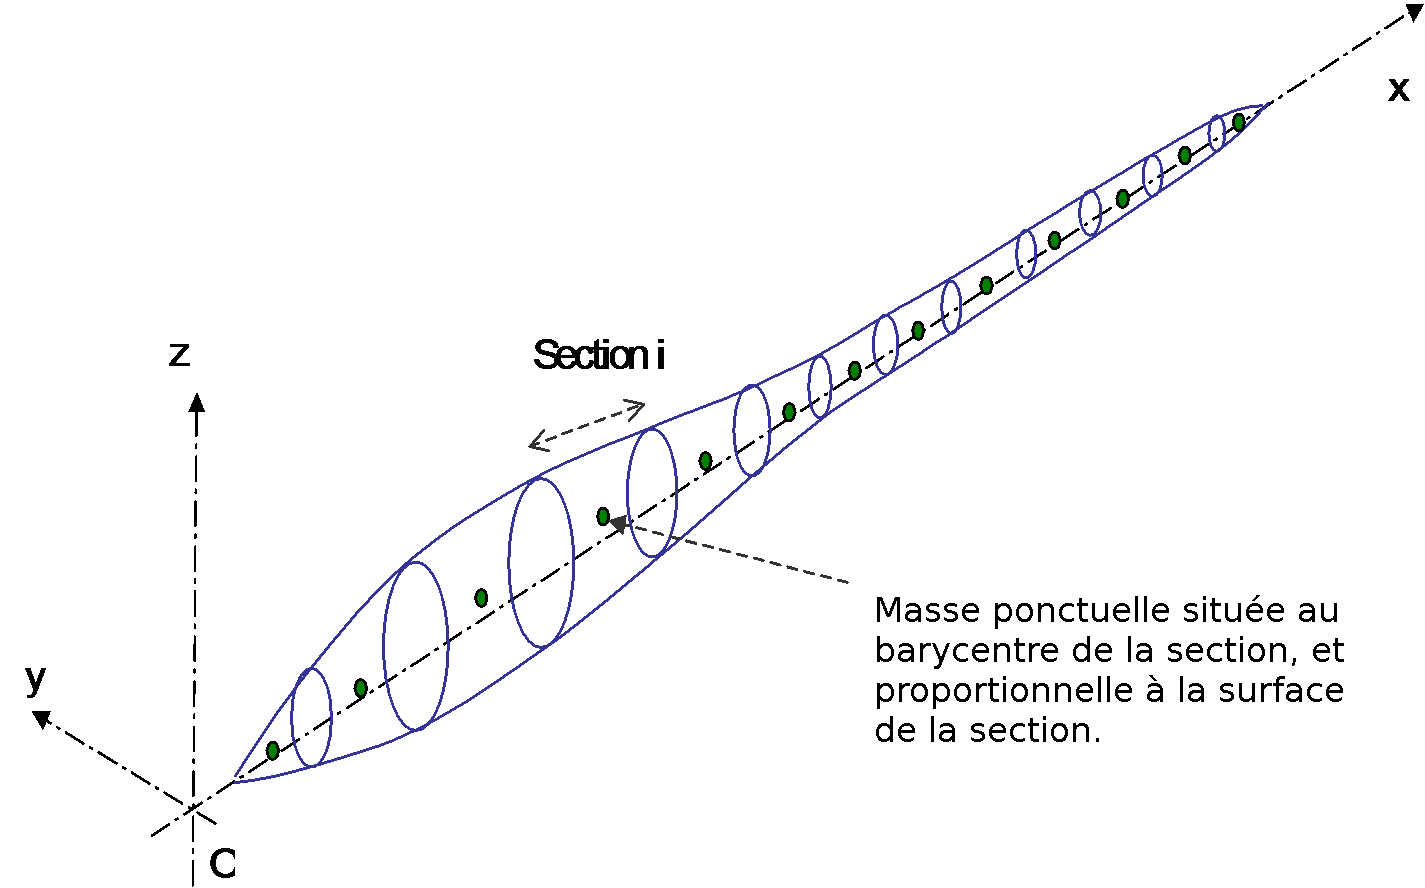
\includegraphics[width=0.8\linewidth]{img-47-fr}
  \caption{Représentation de la masse pour le fuselage}
  \label{img:représentation_masse_fuselage}
\end{figure}

\begin{figure}[htbp]
  \centering
  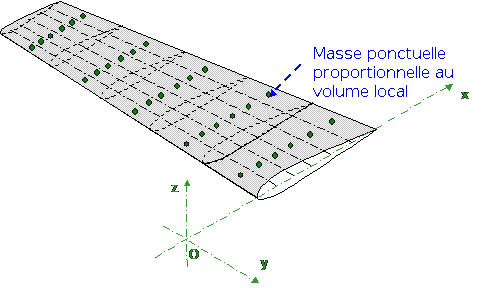
\includegraphics[width=0.8\linewidth]{img-48-fr}
  \caption{Représentation de la masse pour l’aile}
  \label{img:représentation_masse_aile}
\end{figure}

\paragraph{Paramètres des polaires de stabilité}

Les «~polaires de stabilité~» remplacent les précédentes «~polaires de
contrôle~». La différence principale est que la position du CG n’est plus
une variable, mais plutôt déterminée par la distribution des masses dans
l’avion.

L’objet polaire de stabilité prend en entrée~:

\begin{itemize}
  \item la densité et la viscosité dynamique du fluide~;
  \item le type de longueur et de surface de référence pour les calculs
  des paramètres aérodynamiques~;
  \item la sélection de l’analyse soit visqueuse, soit non visqueuse~;
  \item les variables de contrôle à inclure dans l’analyse.
\end{itemize}

\paragraph{Variables de contrôle}

Les points polaires peuvent peuvent être calculés pour différents états
des variables de contrôle. Ces variables sont~:

\begin{itemize}
  \item l’inclinaison de l’aile par rapport à l’axe y~;
  \item l’inclinaison de la profondeur par rapport à l’axe y~;
  \item la rotation des volets de l’aile principale par rapport leur axe
  d’articulation~;
  \item la rotation des volets de la profondeur par rapport à leur axe
  d’articulation~;
  \item la rotation des volet de queue/dérive par rapport à leur axe
  d’articulation.
\end{itemize}

\underline{Notes~:}

\begin{itemize}
	\item Le sens de rotation est positif selon la règle de la main droite, 
	c’est-à-dire~:
	\begin{itemize}
		\item pour l’aile et la profondeur, une valeur positive va déplacer le 
		bord d’attaque vers le haut et le bord de fuite vers le bas~;
		\item pour un volet d’aile ou de profondeur, un valeur de contrôle 
		positive va déplacer le bord de fuite vers le bas~;
		\item pour la dérive, une valeur positive de la commande va déplacer le
		bord de fuite vers tribord.
	\end{itemize}
	
	\item Pour représenter les ailerons qui pivotant dans les sens opposés, les 
	valeurs min et max des commandes pour chacun des ailerons des ailes devront 
	être opposées.
	\item La valeur individuelle de l’angle de commande n’est pas prise en 
	compte dans l’analyse. Par exemple, si le volet a été défini avec les 
	profils avec un angle de volet non nul, les angles initiaux ont été définis
	avec des  angles de volets non nuls, les angles initiaux seront annulés 
	avant de définir la position des commandes.\\
	De même, l’angle d’inclinaison de l’aile ou du volet dans la définition de 
	l’avion est annulé avant l’application de la déflexion~;
	\item Pour une polaire de contrôle, tous les paramètres varient 
	simultanément en accord avec la valeur du paramètre de contrôle «~c~»~:
	$$Variable\_controle = (1-c)~\times~Position\_Min\_controle~+~c
	~\times~Position\_Max\_controle$$
	\item La rotation des commandes n’est pas représentée sur la vue en 3D.
\end{itemize}

\subsubsection{Sortie}

En sortie, le code fournit des résultats pour la dynamique longitudinale et
latérale~:

\begin{itemize}
	\item La stabilité dimensionnelle et les dérivées des contrôles~;
	\item Les dérivées de la stabilité non dimensionnelle~;
	\item Le temps de réponse pour un pas de calcul en d’entrée~;
	\item Les valeurs propres et les vecteurs propres pour les quatre modes 
	longitudinaux et les quatre modes latéraux.
\end{itemize}

\paragraph{Dérivée de la stabilité}

Les dérivées de la stabilité décrivent la modification d’une force ou d’un
moment en réponse à une variation d’une variable de vol. Par exemple, la
variation de la force axiale résultant d’une modification de la vitesse
axiale est~:
$$\frac{\partial F_X}{\partial u} = 
\frac{1}{2}\rho \frac{\partial u_{0}^{2}} S C_X + 
\frac{1}{2}\rho u_{0}^{2} S \frac{\partial C_X}{\partial u}
= \rho u_{0} S C_{X} +
\frac{1}{2} \rho u_{0}^{2} S \frac{\partial C_{X}}{\partial u}$$

Une convention usuelle est d’utiliser des notations simplifiées~:

$$\frac{\partial F_X}{\partial u} = X_u$$

$$\frac{\partial C_X}{\partial u} = Cx_u$$

les deux dérivées étant calculées à l’état d’équilibre.

$X_u$ est la dérivée de la stabilité dimensionnelle, et $Cx_u$ 
la dérivée de la stabilité non dimensionnelle.

XFLR5 calcule les dérivées dimensionnelles qui sont significatives à l’échelle d’un modèle de planeur~:

\begin{itemize}
	\item Dans le sens longitudinal~: $(X_u, X_w, Z_u, Z_w, Z_q, M_u, M_w, M_q)$
	\item Dans le sens latéral~: $(Y_v, Y_p, Y_r, L_v, L_p, L_r, N_v, N_p, N_r)$
\end{itemize}

Les dérivés non dimensionnelles sont habituellement données dans le repère aérodynamique, et les dérivées par rapport à v et w sont fournies à la place de celles par rapport à $\alpha$ et $\beta$. Ce sont~:

\begin{itemize}
  \item Dans le sens longitudinal~: $CL_a, CL_q, Cm_a, Cm_q$,
  \item Dans le sens latéral~: $CY_b, CY_p, CY_r, Cl_b, Cl_p, Cl_r, Cn_b, Cn_p, Cn_r$
\end{itemize}

La définition des dérivés non dimensionnelles est~:

$$CLa = Zw \times u0  / (q \times S)$$

$$CLq = Zq \times 2. \times u0 / (q \times S \times cam)$$

$$Cma = Mw \times u0 / (q \times S \times cam)$$

$$Cmq = Mq \times (2. \times u0 / cam) / (q \times S \times cam)$$

$$CYb = Yv \times u0 / (q \times S)$$

$$CYp = Yp \times  2. \times u0 / (q \times S \times b)$$

$$CYr = Yr \times  2. \times u0 / (q \times S \times b)$$

$$Clb = Lv \times u0 / (q \times S \times b)$$

$$Clp = Lp \times (2. \times u0 / b) /(q \times S \times b)$$

$$Clr = Lr \times (2. \times u0 / b) /(q \times S \times b)$$

$$Cnb = Nv \times u0 / (q \times S \times b)$$

$$Cnp = Np \times (2. \times u0 / b) /(q \times S \times b)$$

$$Cnr = Nr \times (2. \times u0 / b) /(q \times S \times b)$$

Où~:

\begin{tabular}{rl}
  q & est la pression dynamique\\
  S & est la surface de référence\\
  b & est l’envergure de référence\\
  cam & est la corde aérodynamique moyenne.
\end{tabular}

L’évaluation des dérivées est une étape intermédiaire dans les calculs
de la réponse dynamique. Les valeurs de dérivées sont enregistrées
dans l’objet OpPoint, et peuvent être exportées vers un fichier texte
pour l’utiliser dans d’autres codes de simulation de vol.

\paragraph{Modes}

\underline{Modes propres}

D’un point de vue mathématique, la matrice d’état peut être diagonalisée
pour les valeurs propres et les vecteurs propres. Une valeur propre est de
la forme~:

$$\lambda = \sigma + i \omega $$

où~:

\begin{tabular}{rl}
  $\sigma$ & est la constante d’amortissement, unité 1/s\\
  $\omega$ & est la fréquence propre angulaire, unité rad/s
\end{tabular}

Toute valeur propre avec une partie imaginaire non nulle $\omega$, a une valeur propre symétrique donnée par son conjugué. Ceci implique que le temps de réponse d’une variable pour un tel mode est de la forme~:

$$x(t) = R e^{\sigma t} cos(\omega t - \varphi)$$

où $R$ et $\varphi$ sont des valeurs constantes déterminées par les conditions initiales.

Le mode sera dynamiquement stable si l’amortissement est négatif, instable sinon. La stabilité dynamique signifie que lorsqu’il est perturbé, l’avion va retourner progressivement à son état de vol stable.

Autres définitions pour les modes d’oscillation~: $ \omega_1=\sqrt{\lambda
\bar{\lambda}}=\sqrt{\sigma^2 + \omega^2}$ est la fréquence propre angulaire non amortie, unité rad/s.

Pour les modes amortis, c’est-à-dire. $\textstyle \sigma < 0$ , $\zeta = \frac{-\sigma}{\omega_1}$ est le rapport d’amortissement, sans unité~:

\begin{itemize}
	\item $\zeta > 1$ si le mode est sur-amorti~;
	\item $\zeta = 1$ si le mode a un amortissement critique~;
	\item $\zeta < 1$ si me mode est sous-amorti, c’est-à-dire oscillatoire.
\end{itemize}

Si l’amortissement est faible, c’est-à-dire $ \zeta^2 \ll 1$,
alors $\omega_1 \approx \omega$.

La fréquence de vibration du mode (unité Hz) est déterminée par~:

$$F = \omega / 2 \pi $$

La période de temps (unité s) est~:

$$T = 1 / F = 2 \pi / \omega $$

D’un point de vue physique, les valeurs propres et les vecteurs propres
représentent les modes propres sur lesquels l’avion va tendre à osciller.
Pour un problème standard, bien défini, les modes seront~:

\begin{itemize}
	\item Dans le cas longitudinal~:
	\begin{itemize}
		\item deux modes phugoïdes symétriques~;
		\item deux modes symétriques à faible période.
	\end{itemize}
	\item Dans le cas latéral~:
	\begin{itemize}
		\item un mode de roulis amorti~;
		\item un mode de spirale~;
		\item deux modes de roulis hollandais symétriques.
	\end{itemize}
\end{itemize}

\underline{Tracé du lieu des racines}

la position des valeurs propres peut être représenté dans le plan complexe, qui est une manière pratique de vérifier visuellement la stabilité et la fréquence des modes~:

\begin{itemize}
	\item Les racines (valeurs propres) situées sur la gauche du diagramme avec
	une valeur de \texttt{x} négative correspondent à des modes stables, celles
	qui se trouvent sur la partie droite avec des valeurs de \texttt{x} 
	positives, sont instables.\\
	Plus la racine de gauche se trouve basse, plus le mode est stable.
	\item Les racines avec une partie imaginaire non nulle correspondent à des 
	modes oscillatoire, celles avec une partie imaginaire nulle ne sont pas
	oscillatoires.\\
	Plus la racine est éloignée de l’axe x, plus la fréquence d’oscillation est
	élevée.
\end{itemize}

\underline{Forme des modes}

Les valeurs propres définissent la fréquence du mode et son amortissement, et le
vecteur propre en définit la forme.

Ce n’est pas une tâche intuitive de comprendre la forme d’un mode à partir des
composantes du vecteur propre. Une autre manière commode est d’animer le mode dans la vue 3D.

Comme la fréquence et l’amortissement peuvent être très différents d’un mode à l’autre, le temps d’échantillonnage et l’amplitude devront être ajustés pour chaque mode.

L’amplitude \texttt{R} du mode est arbitraire et n’a pas de signification	 physique. Elle peut être ajustée à n’importe quelle valeur pour des raisons d’affichage. En vol, un mode est rarement excité seul. Une perturbation externe tendra plutôt à générer une réponse sur les différents modes longitudinaux et latéraux. Ceci peut être modélisé sur le tracé de temps de réponse.

\paragraph{Temps de réponse}

Le temps de réponse est évalué en se basant sur l’équation de la dynamique
de vol. Par exemple, dans le cas longitudinal, ceci s’exprime par~:

$$\left[\begin{matrix} \dot{u} \\ \dot{w} \\ \dot{q} \\ \dot{\theta} \end{matrix}\right] = \left[A_{long}\right] . \left[\begin{matrix} u \\ w \\  \\ \theta \end{matrix}\right] + \left[B_{long}\right] . \left[F(t)\right]$$

où~:

\begin{tabular}{rl}
  $\left[A_{long}\right]$ & est la matrice d’état $4\times 4$ longitudinale\\
  $\left[B_{long}\right]$ & est la matrice de contrôle d’influence $4 \times n$,
  avec n étant le nombre de variables de contrôle\\
  $\left[F(t)\right]$ & est la matrice $n\times 1$, donnant l’historique de 
  l’entrée forcée pour chaque variable de contrôle
\end{tabular}

De même pour les modes latéraux~:

$$\left[\begin{matrix} \dot{v} \\ \dot{p} \\ \dot{r} \\ \dot{\varphi}
\end{matrix}\right] = \left[A_{lat}\right] . \left[\begin{matrix} v \\ p \\ r \\ \varphi \end{matrix}\right] + \left[B_{lat}\right] . \left[F(t)\right]$$

L’évolution dans le temps des variables d’état (u, w, q, $\theta$) et (v, p, r,
$\varphi$) peut être calculé soit~:
\begin{itemize}
	\item comme une conséquence des conditions initiales perturbées~: il s’agit
	de la «~Réponse aux conditions initiales~»~;
	\item soit comme une conséquence d’une commande de servo en fonction du 
	temps~: il s’agit de la «~Réponse forcée~».
\end{itemize}

\subparagraph{Réponse aux conditions initiales}

L’entrée requise est un échelon de modification depuis l’état d’équilibre du vol. Dans le cas longitudinal, cette entrée peut être fournie par une combinaison quelconque de valeurs pour u, w, et q. Dans le cas latéral, c’est entré comme une combinaison de valeurs de v, p, et r.

\subparagraph{Réponse forcée en boucle ouverte}

Ce type d’analyse effectue l’investigation des réponses de l’avion à une modification d’un paramètre de contrôle. De tels paramètres sont typiquement une
modification de poussée, ou l’activation d’une surface de commande comme la profondeur, la dérive ou les ailerons. La  modification de poussée n’est pas prise en compte par XFLR5.

L’entrée requise est l’évolution dans le temps d’un paramètre de contrôle. XFLR5 n’offre que la possibilité de simuler une rampe linéaire d’une commande pendant une durée finie.

\begin{figure}[htbp]
	\centering
	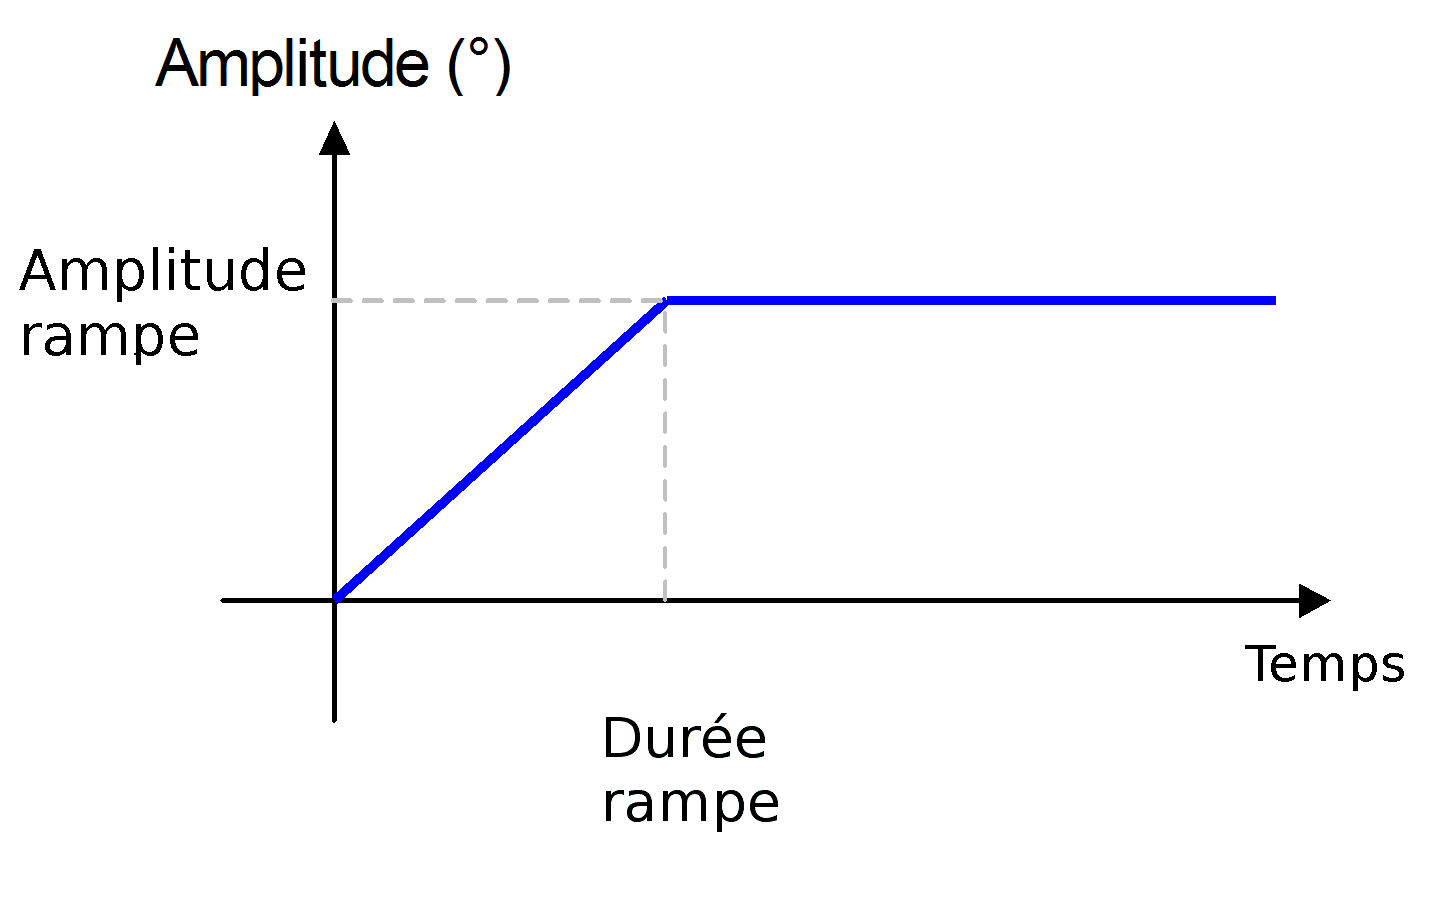
\includegraphics[width=0.8\linewidth]{img-49-fr}
	\caption{Illustration de la rampe de sollicitation}
	\label{img:rampe sollicitation}
\end{figure}

Bien que toutes les variables de contrôle soient définies simultanément pour déterminer la géométrie de l’état stable et les conditions de réglage, la variation de chacune peut être effectuée indépendamment dans l’évaluation de la réponse forcée. Le temps de la rampe est cependant le même pour toutes les variables de contrôle.

Note importante~: l’analyse d’une réponse à une entrée d’échelon longitudinal peut avoir une signification physique car l’avion peut finir par retourner à un état stable proche des conditions initiales. À l’opposé, l’actionnement d’un contrôle latéral conduira à une divergence depuis les conditions d’état stable, à un couplage entre les modes longitudinal et latéral, et l’analyse ne sera pas représentative. Par exemple, les ailerons vont générer un angle d’inclinaison, modifier la portance verticale, et vont conduire à une divergence depuis les conditions d’état stable. Il se passe la même chose pour l’actionnement de la dérive, qui va donner, par exemple, une inclinaison par l’intermédiaire de l’effet du dièdre.

\subsubsection{Exemple de session — Analyse de stabilité}

Suivez les étapes de 1 à 8 comme dans la session d’analyse de l’aile décrite 
dans \S\ref{section : exemple session analyse aile}.

\begin{enumerate}
	\setcounter{enumi}{8}
	\item Optionnel, mais recommandé~: définir les propriétés d’inertie de 
	l’objet avion ou aile actuel.

	\begin{itemize}
		\item Sélectionner l’avion (ou l’aile) actuel / Définir l’inertie~;
		\item Entrer les propriétés d’inertie pour l’avion ou l’aile~;
		\item Assurez-vous que la position du CG se trouve où elle est censée 
		l’être. Il peut être nécessaire de tricher un peu sur les positions des
		masses ponctuelles pour obtenir la position désirée~;
		\item Fermer la boîte de dialogue.
	\end{itemize}
	
	\item Optionnel~: cliquer «~Définir Analyse/Polaire~» depuis le menu 
	Polaire/Aile~;

	\begin{itemize}
		\item Sélectionner une polaire de Type 1 ou de Type 2~;
		\item Sélectionner «~Utiliser l’inertie de l’avion~», si elle a été 
		précédemment définie~;
		\item Lancer une analyse séquentielle depuis les faibles jusqu’aux forts
		angles d’attaque~;
		\item Tracer le graphique $ICm=f(\alpha)$, assurez-vous que la pente est
		 négative et qu’il a des angles d’attaque pour lesquels $ICm=0$
	\end{itemize}

	\item Cliquer «~Définir une analyse de stabilité~» depuis le menu Analyse/
	Stabilité, ou entrer \touche {Maj} + \touche{F6}
	\item Décider soit d’utiliser l’objet inertie précédemment défini, soit 
	d’entrer vous-même la masse, la position du CG, et les propriétés 
	d’inertie~;
	\item Optionnel~: activer une commande et décider de la plage de variation~;
	\item Fermer la boîte de dialogue (presser deux fois \touche{Entrée}). Le 
	nom de la polaire devrait maintenant apparaître dans la boîte combinée en
	haut et au milieu~;
	\item Sélectionner la position du contrôle sur la barre d’outils de droite 
	-- lancer par 0. Désélectionner «~Séquence~»~;
	\item Cocher la case «~Enregistrer l’OpPoint~»~;
	\item Cliquer le bouton \bouton{Analyser} sur la barre d’outils de droite~;
	\item Si l’analyse a été couronnée de succès, un OpPoint est automatiquement
	ajouté dans la boîte combinée en haut et à droite. Sinon, vérifier le 
	fichier journal pour analyser le message d’erreur~;
	\item Sur la vue polaire, cochez la case «~Afficher le point~» de la 
	polaire. Sur le tracé $ICm=f(\alpha)$, le point devait être situé 
	précisément aux conditions de réglage, c’est-à-dire, à l’angle d’attaque 
	pour lequel $ICm=0$~;
	\item Passer à l’analyse de stabilité \touche{Maj}+\touche{F8}~;
	\item Sélectionner soit le tracé du lieu des racines, soit la vue de la 
	réponse en fonction du temps ou la vue 3D.
\end{enumerate}

Poursuivez par la définition de l’analyse de stabilité avec les commandes activées, et visualisez les propriétés de stabilité en fonction de la position de la commande.

\clearpage

\section{Spécificités du code}

\subsection{XFoil, AVL et XFLR5}
XFLR5 a été développé en se basant sur XFoil V6.94. Les éditions ultérieures
de XFoil n’ont pas été incluses dans XFLR5.

Comme les algorithmes ont été ré-écrits et intégrés dans XFLR5, il n’est
pas nécessaire que XFoil soit présent sur l’ordinateur pour que XFLR5
fonctionne. Aucun lien particulier n’a besoin d’être déclaré. XFLR5 n’utilise
aucune partie du code source d’AVL. Les algorithmes VLM ont été développés
et implémentés indépendamment.

Pour les fichiers AVL créés par XFLR5, les noms de profils devront être 
vérifiés, et il sera nécessaire de vérifier aussi que les fichiers de profils 
sont présents dans le répertoire avec les autres fichiers d’AVL. 

\subsection{Fichiers et Registre}

Le lancement de XFLR5 crée en général deux fichiers dans le répertoire de
l’utilisateur pour les fichiers temporaires~:

\begin{itemize}
	\item «~XFLR5.set~» qui conserve les paramètres de l’utilisateur~;
	Supprimez ce fichier pour remettre en place les paramètres par défaut.
	\item «~XFLR5.log~» qui enregistre les sorties des analyses de profils et 
	d’ailes.
\end{itemize}

L’emplacement de ce répertoire est défini par les variables d’environnement de l’utilisateur.

XFLR5 lui-même n’écrit rien dans le registre, mais le programme d’installation va créer les raccourcis pour les fichiers «~.plr~» et «~.wpa~». Les utilisateurs peuvent choisir d’associer les fichiers «~.dat~» de profils à XFLR5, mais comme cette extension est utilisée par Windows pour de nombreuses choses différentes, il a semblé préférable de laisser ce choix à l’utilisateur. Les raccourcis du registre seront supprimés lors du processus de désinstallation\footnote{Ce paragraphe ne concerne que Windows (ndt)}.

\subsection{Raccourcis}

Afin d’améliorer la convivialité de l’interface, des raccourcis ont été fournis pour la plupart des commandes principales et sont mentionnés dans les menus.

Presser une première fois \touche{Entrée} dans une boîte de dialogue va sélectionner \bouton{Valider} ou le bouton par défaut, presser une seconde fois 
\touche{Entrée} va activer ce bouton.

Presser une première fois \touche{Entrée} dans la fenêtre principale va sélectionner le bouton \bouton{Analyser} et presser une seconde fois \touche{Entrée} va activer ce bouton.

\subsection{Entrée à la souris}

Tous les diagrammes, profils et ailes peuvent être glissés et zoomés avec la souris. L’utilisation de \touche{Ctrl}+bouton gauche dans la vue 3D permet la rotation du modèle.

Ces options peuvent cependant ne pas fonctionner correctement (ou pas du tout) si les boutons ne sont pas définis à leur «~Défaut~» dans le paramétrage de la souris de l’interface graphique de votre système.

Presser les touches \touche{X} \touche{Y} lors du zoom d’un diagramme ne l’étendra que sur l’axe correspondant.

Pour les ordinateurs qui n’ont pas de molette de souris, ni de bouton central, le 
zoom peut être obtenu dans toutes les vues en pressant la touche \touche{Z} et en déplaçant la souris. 

\subsection{Mémoire}

Une des caractéristiques des analyses tant des profils que des ailes est d’utiliser une quantité significative de mémoire.

Les points de fonctionnement en particulier, enregistrent une grande quantité de 
données et produisent des fichiers de projet volumineux ce qui ralentit les opérations d’enregistrement et de chargement. Il n’est cependant pas nécessaire de les conserver, car les données importantes sont aussi enregistrées dans les objets polaires qui ne demandent pas de ressources mémoire importantes. 

\subsection{Options d’exportation}
\underline{Impression}

Bien que XFLR5, offre par lui-même certaines options d’impression, 
l’implémentation de possibilités plus avancées demanderait un travail 
conséquent. Il n’a donc pas été, et n’est pas prévu de devenir, le premier
souci des développements en cours.

\underline{Copies d’écran}

Une option a été ajoutée en v4.12 pour exporter les images de l’écran 
client sous forme de fichiers images.

\underline{Données de diagrammes}

Une option a été ajoutée en v4.13 pour exporter les données des diagrammes
dans des fichiers texte.

\underline{Exportation de données}

Tous les résultats, les points de fonctionnements et les polaires peuvent
être exportés dans des fichiers textes afin d’être traité dans des feuilles
de calculs.

Depuis la version v4.12, une option est disponible pour exporter les données
dans le format «~valeurs séparées par des virgules~» «~.csv~». Ce format
texte est destiné à être lu sans conversion dans une feuille de calcul.
Cependant, il peut arriver que les paramètres régionaux de votre système
d’exploitation demandent à être ajustés pour définir la virgule («~,~»)
comme séparateur de liste par défaut. 

\subsection{Bogues}

Une fois encore, XFLR5 n’est en aucune façon un programme professionnel,
et malgré tous les efforts de l’auteur et l’aide de ceux qui l’ont testé et
qui ont fourni des retours appréciables, il n’est très probablement toujours
pas sans défaut.

Corrections des bogues principaux~:
\begin{enumerate}
	\item Dans la méthode des panneaux implémentées dans XFLR5~4, la 
	formulation des condition aux limites de Neumann était incorrecte, ce qui
	conduisait à des résultats incohérents. Pour cette raison, la méthode par
	défaut utilisait les conditions aux limites de Dirichle.\\
	Ce bogue a été corrigé dans XFLR5~v6.02 
	\item Un bogue a été signalé peu de temps après la diffusion de la v3.00,
	le 7 septembre 2006. Il avait pour conséquence majeure de compter deux fois
	la portance de la profondeur dans les calculs d’un avion avec la méthode
	VLM-quad.\\
	Ce bogue a été corrigé dans la version v3.01 diffusée le 24 septembre 2006.
	\item Jusqu’à la version v3.14, la contribution de la profondeur et de la
	dérive aux moments de tangage et de lacet étaient calculés par rapport au
	point X=0 plutôt que X=XCmRef.\\
	Ceci a été corrigé dans la version v3.15 diffusée le 21 janvier 2007.
\end{enumerate}

L’auteur sera très reconnaissant pour tous les signalements de résultats incohérents et autres bogues, et il fera de son mieux pour investiguer et les
corriger rapidement. Pour faciliter les corrections de bogues, les signalements
devraient idéalement comporter~: 

\begin{itemize}
	\item L’identification du système d’exploitation (par exemple Windows XP
	Pro,Vista, Linux, \dots)~;
	\item Le fichier de projet («~xxx.wpa~»)~;
	\item La séquence de commandes ayant conduit au bogue.
\end{itemize}

\subsection{Développement à sources ouvertes}

Le 31 mars 2007, XFLR5 est devenu un projet de développement à sources 
ouvertes hébergé par \href{https://sourceforge.net/projects/xflr5/}
{SourceForge.net}.

SourceForge fournit un ensemble complet d’outils et de méthodes pour le développement de projets et on peut trouver une documentation en ligne. Les contributeurs potentiels qui désireraient aider à organiser le projet, à corriger les bogues ou à ajouter de nouvelles fonctionnalités et améliorations sont les bienvenus.

\section{Remerciements}

Tous mes remerciements à Matthieu pour son avis scientifique et son aide, à Jean-Marc pour sa patience et ses tests complets des versions préliminaires, à Marc pour sa capacité naturelle à déboguer les programmes et les avions, et à tous les autres qui ont contribué par leurs informations à améliorer XFLR5, spécialement Giorgio et Jean-Luc.

Merci aussi à Francesco qui a écrit dans RCSD 2008-04 un tutoriel de qualité pour XFLR5 et qui a aussi contribué au développement de la version pour MacOS.

De même, merci à Karoliina et Jean-Luc pour leur aide dans la compilation de la version Debian/Ubuntu.

Merci aussi à Martin for la traduction en allemand, et à Jean-Luc pour la traduction en français.

\clearpage

%------ REFERENCES --------
\nocite{*}
\bibliography{xflr5} 

%----- LISTE DES TODO -----
%\listoftodos

\clearpage
\listoffigures

\clearpage
\listoftables

\end{document}
